%%%%%%%%%%%%%%%%%%%%%%%%%%%%%%%%%%%%%%%%%%%%%%%%%%%%%%%%%%%%%%%
%% OXFORD THESIS TEMPLATE

% Use this template to produce a standard thesis that meets the Oxford University requirements for DPhil submission
%
% Originally by Keith A. Gillow (gillow@maths.ox.ac.uk), 1997
% Modified by Sam Evans (sam@samuelevansresearch.org), 2007
% Modified by John McManigle (john@oxfordechoes.com), 2015
% Modified by Ulrik Lyngs (ulrik.lyngs@cs.ox.ac.uk), 2018-, for use with R Markdown
%
% Ulrik Lyngs, 25 Nov 2018: Following John McManigle, broad permissions are granted to use, modify, and distribute this software
% as specified in the MIT License included in this distribution's LICENSE file.
%
% John commented this file extensively, so read through to see how to use the various options.  Remember that in LaTeX,
% any line starting with a % is NOT executed.  Several places below, you have a choice of which line to use
% out of multiple options (eg draft vs final, for PDF vs for binding, etc.)  When you pick one, add a % to the beginning of
% the lines you don't want.


%%%%% PAGE LAYOUT
% The most common choices should be below.  You can also do other things, like replacing "a4paper" with "letterpaper", etc.

% This one formats for two-sided binding (ie left and right pages have mirror margins; blank pages inserted where needed):
%\documentclass[a4paper,twoside]{templates/ociamthesis}
% This one formats for one-sided binding (ie left margin > right margin; no extra blank pages):
%\documentclass[a4paper]{ociamthesis}
% This one formats for PDF output (ie equal margins, no extra blank pages):
%\documentclass[a4paper,nobind]{templates/ociamthesis}

% As you can see from the uncommented line below, oxforddown template uses the a4paper size, 
% and passes in the binding option from the YAML header in index.Rmd:
\documentclass[a4paper, nobind]{templates/ociamthesis}


%%%%% ADDING LATEX PACKAGES
% add hyperref package with options from YAML %
\usepackage[pdfpagelabels]{hyperref}
% change the default coloring of links to something sensible
\usepackage{xcolor}

\definecolor{mylinkcolor}{RGB}{0,0,139}
\definecolor{myurlcolor}{RGB}{0,0,139}
\definecolor{mycitecolor}{RGB}{0,33,71}

\hypersetup{
  hidelinks,
  colorlinks,
  linktocpage=true,
  linkcolor=mylinkcolor,
  urlcolor=myurlcolor,
  citecolor=mycitecolor
}



% add float package to allow manual control of figure positioning %
\usepackage{float}

% enable strikethrough
\usepackage[normalem]{ulem}

% use soul package for correction highlighting
\usepackage{color, soul}
\definecolor{correctioncolor}{HTML}{CCCCFF}
\sethlcolor{correctioncolor}
\newcommand{\ctext}[3][RGB]{%
  \begingroup
  \definecolor{hlcolor}{#1}{#2}\sethlcolor{hlcolor}%
  \hl{#3}%
  \endgroup
}
\soulregister\ref7
\soulregister\cite7
\soulregister\autocite7
\soulregister\textcite7
\soulregister\pageref7

%%%%% FIXING / ADDING THINGS THAT'S SPECIAL TO R MARKDOWN'S USE OF LATEX TEMPLATES
% pandoc puts lists in 'tightlist' command when no space between bullet points in Rmd file,
% so we add this command to the template
\providecommand{\tightlist}{%
  \setlength{\itemsep}{0pt}\setlength{\parskip}{0pt}}
 
% UL 1 Dec 2018, fix to include code in shaded environments
\usepackage{color}
\usepackage{fancyvrb}
\newcommand{\VerbBar}{|}
\newcommand{\VERB}{\Verb[commandchars=\\\{\}]}
\DefineVerbatimEnvironment{Highlighting}{Verbatim}{commandchars=\\\{\}}
% Add ',fontsize=\small' for more characters per line
\usepackage{framed}
\definecolor{shadecolor}{RGB}{248,248,248}
\newenvironment{Shaded}{\begin{snugshade}}{\end{snugshade}}
\newcommand{\AlertTok}[1]{\textcolor[rgb]{0.94,0.16,0.16}{#1}}
\newcommand{\AnnotationTok}[1]{\textcolor[rgb]{0.56,0.35,0.01}{\textbf{\textit{#1}}}}
\newcommand{\AttributeTok}[1]{\textcolor[rgb]{0.77,0.63,0.00}{#1}}
\newcommand{\BaseNTok}[1]{\textcolor[rgb]{0.00,0.00,0.81}{#1}}
\newcommand{\BuiltInTok}[1]{#1}
\newcommand{\CharTok}[1]{\textcolor[rgb]{0.31,0.60,0.02}{#1}}
\newcommand{\CommentTok}[1]{\textcolor[rgb]{0.56,0.35,0.01}{\textit{#1}}}
\newcommand{\CommentVarTok}[1]{\textcolor[rgb]{0.56,0.35,0.01}{\textbf{\textit{#1}}}}
\newcommand{\ConstantTok}[1]{\textcolor[rgb]{0.00,0.00,0.00}{#1}}
\newcommand{\ControlFlowTok}[1]{\textcolor[rgb]{0.13,0.29,0.53}{\textbf{#1}}}
\newcommand{\DataTypeTok}[1]{\textcolor[rgb]{0.13,0.29,0.53}{#1}}
\newcommand{\DecValTok}[1]{\textcolor[rgb]{0.00,0.00,0.81}{#1}}
\newcommand{\DocumentationTok}[1]{\textcolor[rgb]{0.56,0.35,0.01}{\textbf{\textit{#1}}}}
\newcommand{\ErrorTok}[1]{\textcolor[rgb]{0.64,0.00,0.00}{\textbf{#1}}}
\newcommand{\ExtensionTok}[1]{#1}
\newcommand{\FloatTok}[1]{\textcolor[rgb]{0.00,0.00,0.81}{#1}}
\newcommand{\FunctionTok}[1]{\textcolor[rgb]{0.00,0.00,0.00}{#1}}
\newcommand{\ImportTok}[1]{#1}
\newcommand{\InformationTok}[1]{\textcolor[rgb]{0.56,0.35,0.01}{\textbf{\textit{#1}}}}
\newcommand{\KeywordTok}[1]{\textcolor[rgb]{0.13,0.29,0.53}{\textbf{#1}}}
\newcommand{\NormalTok}[1]{#1}
\newcommand{\OperatorTok}[1]{\textcolor[rgb]{0.81,0.36,0.00}{\textbf{#1}}}
\newcommand{\OtherTok}[1]{\textcolor[rgb]{0.56,0.35,0.01}{#1}}
\newcommand{\PreprocessorTok}[1]{\textcolor[rgb]{0.56,0.35,0.01}{\textit{#1}}}
\newcommand{\RegionMarkerTok}[1]{#1}
\newcommand{\SpecialCharTok}[1]{\textcolor[rgb]{0.00,0.00,0.00}{#1}}
\newcommand{\SpecialStringTok}[1]{\textcolor[rgb]{0.31,0.60,0.02}{#1}}
\newcommand{\StringTok}[1]{\textcolor[rgb]{0.31,0.60,0.02}{#1}}
\newcommand{\VariableTok}[1]{\textcolor[rgb]{0.00,0.00,0.00}{#1}}
\newcommand{\VerbatimStringTok}[1]{\textcolor[rgb]{0.31,0.60,0.02}{#1}}
\newcommand{\WarningTok}[1]{\textcolor[rgb]{0.56,0.35,0.01}{\textbf{\textit{#1}}}}

%UL set white space before and after code blocks
\renewenvironment{Shaded}
{
  \vspace{10pt}%
  \begin{snugshade}%
}{%
  \end{snugshade}%
  \vspace{8pt}%
}

% User-included things with header_includes or in_header will appear here
% kableExtra packages will appear here if you use library(kableExtra)
\usepackage{booktabs}
\usepackage{longtable}
\usepackage{array}
\usepackage{multirow}
\usepackage{wrapfig}
\usepackage{float}
\usepackage{colortbl}
\usepackage{pdflscape}
\usepackage{tabu}
\usepackage{threeparttable}
\usepackage{threeparttablex}
\usepackage[normalem]{ulem}
\usepackage{makecell}
\usepackage{xcolor}


%UL set section header spacing
\usepackage{titlesec}
% 
\titlespacing\subsubsection{0pt}{24pt plus 4pt minus 2pt}{0pt plus 2pt minus 2pt}


%UL set whitespace around verbatim environments
\usepackage{etoolbox}
\makeatletter
\preto{\@verbatim}{\topsep=0pt \partopsep=0pt }
\makeatother



%%%%%%% PAGE HEADERS AND FOOTERS %%%%%%%%%
\usepackage{fancyhdr}
\setlength{\headheight}{15pt}
\fancyhf{} % clear the header and footers
\pagestyle{fancy}
\renewcommand{\chaptermark}[1]{\markboth{\thechapter. #1}{\thechapter. #1}}
\renewcommand{\sectionmark}[1]{\markright{\thesection. #1}} 
\renewcommand{\headrulewidth}{0pt}

\fancyhead[LO]{\emph{\leftmark}} 
\fancyhead[RE]{\emph{\rightmark}} 

% UL page number position 
\fancyfoot[C]{\emph{\thepage}} %regular pages
\fancypagestyle{plain}{\fancyhf{}\fancyfoot[C]{\emph{\thepage}}} %chapter pages

% JEM fix header on cleared pages for openright
\def\cleardoublepage{\clearpage\if@twoside \ifodd\c@page\else
   \hbox{}
   \fancyfoot[C]{}
   \newpage
   \if@twocolumn\hbox{}\newpage
   \fi
   \fancyhead[LO]{\emph{\leftmark}} 
   \fancyhead[RE]{\emph{\rightmark}} 
   \fi\fi}


%%%%% SELECT YOUR DRAFT OPTIONS
% This adds a "DRAFT" footer to every normal page.  (The first page of each chapter is not a "normal" page.)

% IP feb 2021: option to include line numbers in PDF

% for line wrapping in code blocks
\usepackage{fvextra}
\DefineVerbatimEnvironment{Highlighting}{Verbatim}{breaklines,commandchars=\\\{\}}

% This highlights (in blue) corrections marked with (for words) \mccorrect{blah} or (for whole
% paragraphs) \begin{mccorrection} . . . \end{mccorrection}.  This can be useful for sending a PDF of
% your corrected thesis to your examiners for review.  Turn it off, and the blue disappears.
\correctionstrue


%%%%% BIBLIOGRAPHY SETUP
% Note that your bibliography will require some tweaking depending on your department, preferred format, etc.
% If you've not used LaTeX before, I recommend reading a little about biblatex/biber and getting started with it.
% If you're already a LaTeX pro and are used to natbib or something, modify as necessary.
% Either way, you'll have to choose and configure an appropriate bibliography format...


\usepackage[style=numeric-comp, sorting=none]{biblatex}
\newcommand*{\bibtitle}{References}

\addbibresource{bibliography/references.bib}
\addbibresource{bibliography/additional-references.bib}


% This makes the bibliography left-aligned (not 'justified') and slightly smaller font.
\renewcommand*{\bibfont}{\raggedright\small}


% Uncomment this if you want equation numbers per section (2.3.12), instead of per chapter (2.18):
%\numberwithin{equation}{subsection}


%%%%% THESIS / TITLE PAGE INFORMATION
% Everybody needs to complete the following:
\title{Dynamics of Learning Beyond Stochastic Gradient Descent\\}
\author{Doğan Can Demirbilek}
\college{}

% Master's candidates who require the alternate title page (with candidate number and word count)
% must also un-comment and complete the following three lines:

% Uncomment the following line if your degree also includes exams (eg most masters):
%\renewcommand{\submittedtext}{Submitted in partial completion of the}
% Your full degree name.  (But remember that DPhils aren't "in" anything.  They're just DPhils.)
\degree{Master in Data Science and Scientific Computing}
% Term and year of submission, or date if your board requires (eg most masters)
\degreedate{December 2021}


%%%%% YOUR OWN PERSONAL MACROS
% This is a good place to dump your own LaTeX macros as they come up.

% To make text superscripts shortcuts
	\renewcommand{\th}{\textsuperscript{th}} % ex: I won 4\th place
	\newcommand{\nd}{\textsuperscript{nd}}
	\renewcommand{\st}{\textsuperscript{st}}
	\newcommand{\rd}{\textsuperscript{rd}}

%%%%% THE ACTUAL DOCUMENT STARTS HERE
\begin{document}

%%%%% CHOOSE YOUR LINE SPACING HERE
% This is the official option.  Use it for your submission copy and library copy:
\setlength{\textbaselineskip}{22pt plus2pt}
% This is closer spacing (about 1.5-spaced) that you might prefer for your personal copies:
%\setlength{\textbaselineskip}{18pt plus2pt minus1pt}

% You can set the spacing here for the roman-numbered pages (acknowledgements, table of contents, etc.)
\setlength{\frontmatterbaselineskip}{17pt plus1pt minus1pt}

% UL: You can set the line and paragraph spacing here for the separate abstract page to be handed in to Examination schools
\setlength{\abstractseparatelineskip}{13pt plus1pt minus1pt}
\setlength{\abstractseparateparskip}{0pt plus 1pt}

% UL: You can set the general paragraph spacing here - I've set it to 2pt (was 0) so
% it's less claustrophobic
\setlength{\parskip}{2pt plus 1pt}

%
% Oxford University logo on title page
%
\def\crest{{
\includegraphics[width=5cm]{figures/logo.jpeg}}}
\renewcommand{\university}{University of Trieste}
\renewcommand{\submittedtext}{}


% Leave this line alone; it gets things started for the real document.
\setlength{\baselineskip}{\textbaselineskip}


%%%%% CHOOSE YOUR SECTION NUMBERING DEPTH HERE
% You have two choices.  First, how far down are sections numbered?  (Below that, they're named but
% don't get numbers.)  Second, what level of section appears in the table of contents?  These don't have
% to match: you can have numbered sections that don't show up in the ToC, or unnumbered sections that
% do.  Throughout, 0 = chapter; 1 = section; 2 = subsection; 3 = subsubsection, 4 = paragraph...

% The level that gets a number:
\setcounter{secnumdepth}{2}
% The level that shows up in the ToC:
\setcounter{tocdepth}{1}


%%%%% ABSTRACT SEPARATE
% This is used to create the separate, one-page abstract that you are required to hand into the Exam
% Schools.  You can comment it out to generate a PDF for printing or whatnot.

% JEM: Pages are roman numbered from here, though page numbers are invisible until ToC.  This is in
% keeping with most typesetting conventions.
\begin{romanpages}

% Title page is created here
\input{templates/alternative\_cover.tex}

%%%%% DEDICATION -- If you'd like one, un-comment the following.
\begin{dedication}
  \emph{To my family}
\end{dedication}

%%%%% ACKNOWLEDGEMENTS -- Nothing to do here except comment out if you don't want it.
\begin{acknowledgements}
 	This is where you will normally thank your advisor, colleagues, family and friends, as well as funding and institutional support. In our case, we will give our praises to the people who developed the ideas and tools that allow us to push open science a little step forward by writing plain-text, transparent, and reproducible theses in R Markdown.

We must be grateful to John Gruber for inventing the original version of Markdown, to John MacFarlane for creating Pandoc (\url{http://pandoc.org}) which converts Markdown to a large number of output formats, and to Yihui Xie for creating \texttt{knitr} which introduced R Markdown as a way of embedding code in Markdown documents, and \texttt{bookdown} which added tools for technical and longer-form writing.

Special thanks to \href{http://chester.rbind.io}{Chester Ismay}, who created the \texttt{thesisdown} package that helped many a PhD student write their theses in R Markdown. And a very special thanks to John McManigle, whose adaption of Sam Evans' adaptation of Keith Gillow's original maths template for writing an Oxford University DPhil thesis in LaTeX provided the template that I in turn adapted for R Markdown.

Finally, profuse thanks to JJ Allaire, the founder and CEO of \href{http://rstudio.com}{RStudio}, and Hadley Wickham, the mastermind of the tidyverse without whom we'd all just given up and done data science in Python instead. Thanks for making data science easier, more accessible, and more fun for us all.

\begin{flushright}
Ulrik Lyngs \\
Linacre College, Oxford \\
2 December 2018
\end{flushright}
\end{acknowledgements}


%%%%% ABSTRACT -- Nothing to do here except comment out if you don't want it.
\begin{abstract}
	This \emph{R Markdown} template is for writing an Oxford University thesis. The template is built using Yihui Xie's \texttt{bookdown} package, with heavy inspiration from Chester Ismay's \texttt{thesisdown} and the \texttt{OxThesis} \LaTeX~template (most recently adapted by John McManigle).

This template's sample content include illustrations of how to write a thesis in R Markdown, and largely follows the structure from \href{https://ulyngs.github.io/rmarkdown-workshop-2019/}{this R Markdown workshop}.

Congratulations for taking a step further into the lands of open, reproducible science by writing your thesis using a tool that allows you to transparently include tables and dynamically generated plots directly from the underlying data. Hip hooray!
\end{abstract}

%%%%% MINI TABLES
% This lays the groundwork for per-chapter, mini tables of contents.  Comment the following line
% (and remove \minitoc from the chapter files) if you don't want this.  Un-comment either of the
% next two lines if you want a per-chapter list of figures or tables.
  \dominitoc % include a mini table of contents

% This aligns the bottom of the text of each page.  It generally makes things look better.
\flushbottom

% This is where the whole-document ToC appears:
\tableofcontents

\listoffigures
	\mtcaddchapter
  	% \mtcaddchapter is needed when adding a non-chapter (but chapter-like) entity to avoid confusing minitoc

% Uncomment to generate a list of tables:
\listoftables
  \mtcaddchapter
%%%%% LIST OF ABBREVIATIONS
% This example includes a list of abbreviations.  Look at text/abbreviations.tex to see how that file is
% formatted.  The template can handle any kind of list though, so this might be a good place for a
% glossary, etc.
% First parameter can be changed eg to "Glossary" or something.
% Second parameter is the max length of bold terms.
\begin{mclistof}{List of Abbreviations}{3.2cm}

\item[ANN]

Artificial Neural Network.

\item[BP]

Backpropagation.

\item[DFA]

Direct Feedback Alignment.

\item[BCE]

Binary Cross Entropy.

\item[FA]

Feedback Alignment.

\item[NTK]

Neural Tangent Kernel.

\item[t-SNE]

t-Distributed Stochastic Neighbor Embedding.

\item[SGD]

Stochastic Gradient Descent.

\item[NAG]

Nesterov Accelerated Gradient.

\end{mclistof} 


% The Roman pages, like the Roman Empire, must come to its inevitable close.
\end{romanpages}

%%%%% CHAPTERS
% Add or remove any chapters you'd like here, by file name (excluding '.tex'):
\flushbottom

% all your chapters and appendices will appear here
\hypertarget{introduction}{%
\chapter*{Introduction}\label{introduction}}
\addcontentsline{toc}{chapter}{Introduction}

\adjustmtc
\markboth{Introduction}{}

Artificial neural networks (ANNs) are a collection of connected computational nodes inspired by biological neural networks. Each connection can transmit a helpful signal to another computational node like synapses in a brain. ANNs demonstrated colossal advancements in the last decades. Thanks to these advancements, it is possible to solve complex problems in computer vision, speech recognition, and natural language processing within a reasonable amount of time and with satisfactory performance. These advancements were actualized through an old but robust algorithm called backpropagation (BP). BP is a training algorithm for ANNs that is based on repeatedly adjusting network weights to minimize the difference (loss) between the output of the network and the ground truth \cite{Rumelhart:1986we}.\\
Although nowadays BP is the workhorse algorithm for training ANNs, it has some drawbacks, and it is not the only alternative. Recent studies offered different algorithms to train ANNs by addressing these drawbacks. These algorithms have other properties and principles than BP. Some of them are competitive with BP, or they even outperform the BP in terms of performance or convergence speed for specific problems.\\
This thesis investigates the learning structures through BP and one of the alternative algorithm called direct feedback alignment (DFA) on the particular problem. Unlike BP, the error is propagated through a fixed random matrix instead of the layers' weights in DFA. Then network learns how to make this feedback useful. \cite{nøkland2016direct}. Due to this error propagation mechanism, DFA is considered more biologically plausible than BP, and it opens the gate of parallelism in the training phase of ANNs.\\
The problem at hand is known as the parity learning problem. Previous results showed that these parities are learnable by BP and lazy methods in a more simple setting, whereas it is only learnable by BP in a more complex setting \cite{DBLP:journals/corr/abs-2002-07400}. That is why it is intriguing to test alternative algorithms on this problem to understand their learning dynamics and capabilities.\\
The experiment results might lead us to three possible outcomes. First, we might acquire a similar performance as BP. If it is the case, it would be beneficial to test DFA and BP on a more challenging problem for further studies. Second, there might be a gap between BP and DFA then it would be intriguing to understand where the difference is coming from and how we can close this gap. Third, the alternative algorithm might not even learn, and in this case, it is interesting to ask what makes a problem learnable by BP but not DFA. In all cases, results should help to understand the dynamics of learning of both methods.\\
For applying BP and DFA in a more realistic setting, experiments are performed on the MNIST dataset by imitating the parity learning problem. After putting DFA to this frame, the reason behind the results is interpreted, and possible improvements are motivated and implemented.\\
Chapter \ref{chap:chapter_1} constructs the theoretical bases of the algorithms that are used for the experiments. These bases are composed of simple definitions, mathematical foundations, and the drawbacks of the algorithms. They help to dig deeper into the learning structures of the training algorithms. It is expected to have more control over their learning behaviors by tweaking components of these foundations. Also, it is beneficial to have these theoretical bases for acquiring a better understanding of the further interventions. Moreover, these theoretical foundations are used to implement the algorithms from scratch to use in experiments.\\
Chapter \ref{chap:chapter_2} introduces the parity learning problem at hand. First, the formal definition of the problem is demonstrated then how the problem is imitated by using the MNIST dataset is explained in detail. This part is also highly correlated with the training phase of the algorithms. Later experiment results from \cite{DBLP:journals/corr/abs-2002-07400} are replicated to have concrete picture of previous studies.\\
Chapter \ref{chap:chapter_3} presents results of the experiments. After having the same results from the previous studies for the parity problem, DFA is tested on the same problem.\\
Chapter \ref{chap:chapter_4} wraps up the findings from experiments and creates a path for future studies.

\hypertarget{chap:chapter_1}{%
\chapter{Theoretical Foundations}\label{chap:chapter_1}}

\minitoc 

\hypertarget{backpropagation}{%
\section{Backpropagation}\label{backpropagation}}

BP is one of the first algorithms that show ANNs could learn hidden representations well. Numerous studies showed that ANNs trained with BP could capture similar information as biological neural networks (e.g., specific nodes learn the edges, corners). We need three components for BP, a dataset composed of input-output pairs, a network consisting of parameters (weights and biases), and it allows the input to flow through the network to have output. We need a loss function to measure the difference between the output of the network and the ground truth that we have from the dataset.\\
The main goal of BP is computing the gradients of the loss function (a measure of difference) concerning the parameters of neural networks by using the chain rule. These gradients show how much the parameter needs to change (positively or negatively) to minimize the loss function. After efficiently calculating the gradients, we can nudge the network parameters using gradient descent or its variants.\\
Although BP is an older idea, it earned popularity with \cite{Rumelhart:1986we} because it presented how BP can make a network to learn the representations. After this popularity, the community published numerous practical and theoretical papers that investigated the dynamics of BP. It would be repeat and infeasible to show all the aspects again. However, for completeness and a smoother transition from BP to DFA, it is beneficial to have visual and mathematical explanations showing how the algorithms propagate the errors and the weights. For the mathematical foundations, a binary classification task will be demonstrated with binary cross-entropy loss as an example in appendix \ref{chap:appendix_a}. This example is not chosen arbitrarily. Indeed the parity problem that MNIST imitates is a binary classification problem. In addition to this, equations from appendix \ref{chap:appendix_a} are used to implement BP from scratch to have more control over the process. Then the exact implementation is modified to obtain DFA. The same set of steps are valid for different loss functions and activation functions. Only the calculations will be slightly different. The general idea is the same: obtaining the gradients by calculating the derivative of the loss function concerning the parameters.

\begin{figure}

{\centering 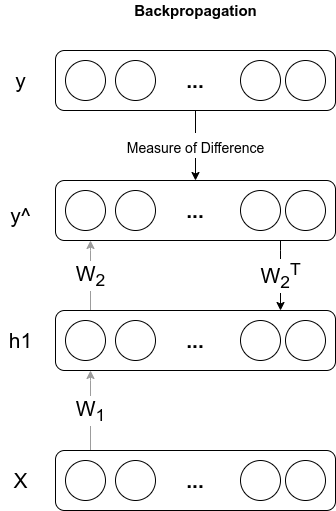
\includegraphics[width=0.3\linewidth]{figures/BP} 

}

\caption{Error Transportation in Backpropagation}\label{fig:BP-Error}
\end{figure}

\noindent In figure \ref{fig:BP-Error} we have a simple network with only a hidden layer that shows the error transportation configuration in BP. \(W_i\) are the weights, \(h_i\) are the output of the hidden layers that is denoted as \(i\), \(\hat{y}\) is the output of the network, and \(y\) is the ground truth, for the sake of simplicity, biases are not showed in this figure. It is important to note that in BP, the transpose of weight is propagated to calculate the gradients. In literature, this issue is known as the weight transport problem, and it is one of the most criticized disadvantages of BP.

\hypertarget{drawbacks-of-bp}{%
\subsection{Drawbacks of BP}\label{drawbacks-of-bp}}

We know that biological neurons inspired ANNs. However, recent studies showed that BP is not precisely how biological neurons learn \cite{bengio2016biologically}. This brings a term called biological plausibility of an algorithm that indicates the algorithm's consistency with existing biological, medical, and neuroscientific knowledge. That is why the community proposed many alternative algorithms by addressing these limitations of BP. In the light of this term, we can put in order the drawbacks of BP as the following:

\begin{itemize}
    \item \textbf{Biological implausibility:}
    \begin{itemize}
        \item The BP computation is purely linear whereas biological neurons interleave linear and non-linear operations.
        \item BP needs precise knowledge of derivatives of the non-linearities at the operating point used in the corresponding feedforward computation on the feedforward path.
        \item BP has to use exact symmetric weights of the feedforward connections.
        \item Real neurons communicate by binary values (spikes), not by clean continuous values.
        \item The computation has to be precisely clocked to alternate between feedforward and BP phases.
        \item It is not clear where the output targets would come from.
        \cite{bengio2016biologically, lee2015difference} 
    \end{itemize}  
    \item \textbf{Vanishing or Exploding Gradients}
    \item \textbf{Lack of Parallel Processing} \cite{ma2019hsic}
\end{itemize}

\noindent Simple interventions may handle some of these drawbacks. For instance, implementing gradient clipping or different activation functions might solve exploding gradients and vanishing gradients. However, they may frequently happen in deeper networks, and they must be considered while training ANNs. On the other hand, some of the drawbacks can not be handled with superficial modifications. For instance, BP is a sequential process, and there are locking mechanisms (forward, backward and update) that ensure none of the processes is executed before its preceding completion. This makes BP infeasible for parallel processing because each execution has to wait for its preceding process. Hence deeper and larger networks' training can be computationally expensive.\\
Biological plausibility is significant because of a couple of reasons. We know that biological neurons inspired ANNs, and biological plausibility refers to consistency between BP and biological knowledge about the neurons of a brain. Hence, it is interesting to examine the dissimilarity or similarity among them. Besides, there is a field that is the intersection of neuroscience and deep learning, so it is natural to investigate the biological plausibility feature of the algorithms, especially for this field. Furthermore, even though nowadays ANNs might outperform the human brain in a specific task, we are still distant from fully mimicking it. In other words, most of the time, ANNs are very good on a task that they are trained in, but they are not diverse, and some kinds of attacks like adversarial ones can easily trick them. Investigating the learning dynamics of these algorithms may open the doors of diverse ANNs that are not specialized in a single task or make them more robust to attacks.\\
Alternative algorithms address some of the drawbacks of BP, and they propose a solution to them, but they also demonstrate a couple of them. However, these algorithms can be considered one or more steps closer to more biologically plausible and robust algorithms.

\hypertarget{direct-feedback-alignment}{%
\section{Direct Feedback Alignment}\label{direct-feedback-alignment}}

So far, we have seen how the error is propagated in BP sequentially through a network with the backward pass. Unlike BP, DFA uses a different way to propagate the error. This way uses a random matrix instead of the transpose of the weight matrix, which brings a solution to the weight transport problem. Before explaining how DFA works, it is better to investigate the feedback alignment (FA) algorithm since DFA is the extension of FA.\\
In \cite{lillicrap2014random}, authors proved that precise symmetric weights are not required to obtain learning in ANNs. Without these matrices, BP-like learning can be obtained. Any random matrix under some conditions can provide the learning. Implicit dynamics in the standard forward weight updates encourage an alignment between weights and the random matrix. In other words, a random matrix pushes the network in roughly the same direction as BP would. They supported this hypothesis with some experiments on a linear problem and MNIST classification task. The empirical results demonstrate that FA successfully trains the network and has similar performance results as BP on these tasks.\\
Even though learning still occurs with random matrix and FA offers the solution to the weight transport problem, it does not provide any computational advantage. To extend DFA, we need to change the error propagation mechanism of FA slightly. In FA, the error is propagated through a random matrix, but the backward process is still sequential. DFA extends this idea and propagates the random matrix in parallel to each layer. In other words, DFA takes the loss and distribute it globally to all layers without requiring sequential step. It also creates an opportunity to parallelize the computation that might speed up the training process.

\begin{figure}

{\centering 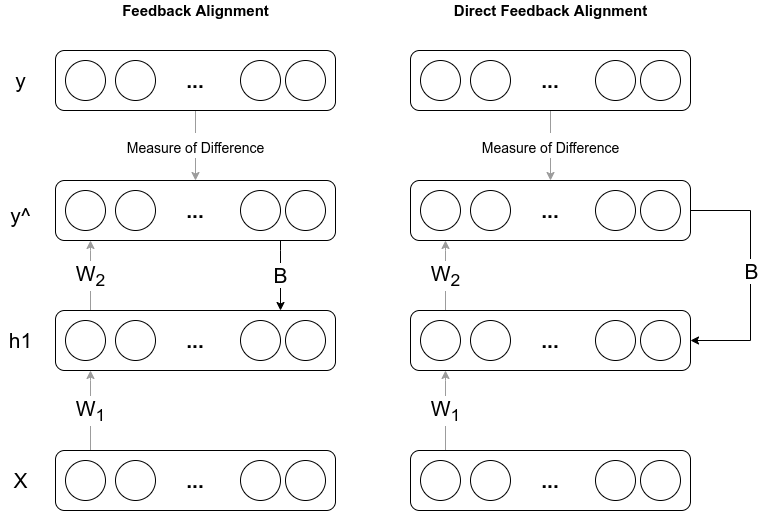
\includegraphics[width=0.65\linewidth]{figures/DFA} 

}

\caption{Error Transportation in Direct Feedback Alignment}\label{fig:DFA-Error}
\end{figure}

\noindent In figure \ref{fig:DFA-Error} we can see the error transportation configurations for FA and DFA. This figure is the same as the one in \cite{nøkland2016direct} but shows only one hidden layer. In fact, with only one hidden layer, FA and DFA are identical.\\
It is crucial to point out, BP and DFA have different learning dynamics. BP calculates the gradients that point to the steepest descent in the loss function space. On the other hand, FA and DFA provide a different update direction but still descending. It is still descending because empirical and theoretical results proved that the networks' weights align with the random matrix that leads to gradients alignment. Therefore the more alignment we have, the same direction would FA and DFA point as BP. Even though they have different update directions, since they are both descending, the results from \cite{lillicrap2014random, nøkland2016direct} showed that FA and DFA are as good as BP in terms of performance for specified tasks in these papers. In addition to this, ANNs trained with DFA show decent separation for labels as in BP's hidden representations of the layers. We can observe this from the t-distributed stochastic neighbor embedding (t-SNE) visualizations of the hidden layers' representations. t-SNE is a method visualizing high-dimensional data which tries to keep the neighbor property in lower dimensions.\\
Recently, a new study has been published which tests the applicability of DFA on modern deep learning tasks and architectures such as neural view synthesis, recommender systems, geometric learning, and natural language processing \cite{launay2020direct}. Because even though some of the alternative methods are competitive with BP in simple tasks like MNIST, they are not competitive or trainable on more complex tasks. Results showed that DFA successfully trains all these complex architectures with performance close to BP. This study supports that complex tasks can be solved without symmetric weight transport, proving that DFA is suitable for more challenging problems.\\
Let us use the same example as \ref{chap:appendix_a} to present how gradients are calculated in DFA. After having the mathematical foundations of BP, transition to DFA is relatively easy. The forward pass is the same as BP, whereas, in the backward pass, we need to replace the transpose of the weight matrix, which is used to calculate the gradients with the random matrix. Considering the same example, we have a simple binary classification task with binary cross-entropy loss, and our network has only one hidden layer. In this setting, gradients of the weights can be calculated as the following:
\[
\frac{\partial BCE}{\partial w_{2}}=h_{1}^T\left(\hat{y}-y\right)
\]
There is no change in the calculations of gradients of the last layer, whereas, for the hidden layer, we have:
\[
\begin{aligned}
\frac{\partial BCE}{\partial w_{1}}= \left(X\right)^T\left(\hat{y}-y\right)\left(B\right) \odot f'(a_1)
\end{aligned}
\]
Please pay attention that \(w_2^T\) is replaced with the random matrix \(B\). This means that we can obtain learning by changing either the random matrix or weight matrix. We know that in DFA, \(B\) is fixed, so the feedforward weights of the network will learn to make these signals useful by aligning with the BP's teaching signal.\\
Update rules are the same as BP, which means that gradient descent and its variants can be used.
\[
\begin{aligned} 
\text{parameter} &= \text{parameter} - \text{step size} \times \frac{\partial BCE}{\partial \text(parameter)}  \\
\end{aligned}
\]
With this tiny modification, DFA brings a solution to some of the drawbacks of BP. Such as using exact symmetric weights of the feedforward connections (weight transport problem), lack of parallel processing (random matrix can be propagated in parallel), and it is less likely to suffer from vanishing or exploding gradients than BP. Eventually, it proposes a more biologically plausible training method. However, it is not the perfect solution either. Because it assumes there is a global feedback path to propagate the error that might be biologically implausible because feedback has to travel a long physical distance. It also suffers some of the drawbacks of BP. For instance, computation is still purely linear. We still need precise knowledge of derivatives of non-linearities. We still communicate by clean, continuous values, and it is unclear where the output targets would come from. Besides, DFA has an extra task to accomplish while training the ANN that aligns with BP's weights, and a layer can not learn before its preceding layers are aligned. This might spawn performance concerns, and DFA might lag behind BP.
Furthermore, DFA fails to train convolutional neural networks which dominate the computer vision tasks \cite{refinetti2021align, launay2019principled}. Finally, unlike BP, DFA was not investigated on particular subjects like adversarial attacks and interpretability by the community. This leaves some question marks about the robustness of DFA.

\hypertarget{lazy-methods}{%
\section{Lazy Methods}\label{lazy-methods}}

Theoretical results present that especially over-parameterized ANNs (not limited to these networks) trained with gradient-based methods can reach zero training loss with their parameters barely changing. The term lazy does not refer to the poor property of methods, whereas they are called lazy methods because their parameters hardly move during training \cite{chizat2020lazy}.\\
Lazy methods are not at the center of the experiments. Hence, detailed explanations of these methods are out of scope in this study, but they have been presented in \cite{DBLP:journals/corr/abs-2002-07400}, and they fail to learn the parities in a more complex setting. Hence, they are implemented too for completeness, and it is essential to embody at least a simple definition of them and how they are practically implemented.

\hypertarget{neural-tangent-kernel}{%
\subsection{Neural Tangent Kernel}\label{neural-tangent-kernel}}

Studies showed that neural networks under some conditions are equivalent to gaussian process, and they mathematically approximate the kernel machines if they are trained with gradient descent \cite{lee2018deep, domingos2020model}. Authors of \cite{DBLP:journals/corr/abs-1806-07572} proved that during the training phase, ANNs follow the kernel gradient of the functional loss concerning a new kernel. They named this kernel a Neural Tangent Kernel (NTK). In other words, NTK is a kernel that describes the evolution of an ANN during the learning phase and, it is beneficial to explain the training of ANNs in function space rather than parameters space. It allows us to work with infinite width neural networks using the kernel trick, and it helps us understand the dynamics of learning and interference.\\
Empirical results demonstrated that the NTK regime performs worse than BP on standard tasks like MNIST. However, NTK is still worth investigating further to understand ANNs' training dynamics since it brings a new perspective on the training phase.\\
Basic practical implementation of NTK is obtained with three steps. Initially, an extra layer is created with the exact dimensions of the first layer. The second in the forward pass concatenation of these two layers' parameters are given as input to the gated linear unit with \(1\). Lastly, in the parameters update phase, the extra layer is not considered. With these adjustments, we decoupled the gating from the linearity of the ReLU, and we kept the gates fixed during training.

\hypertarget{random-features}{%
\subsection{Random features}\label{random-features}}

Standard random features are where first layer weights are initialized randomly by following a distribution and the train only the second layer. These mechanisms are particularly good at approximating kernels. They are preferred because kernel machines might take too much time to train if the data size is big. In \textbf{gaussian features} case, we initialize the first layer weights using gaussian distribution. In contrast, in \textbf{ReLU features} and \textbf{linear features}, we initialize the first layer weights uniformly but, for linear features, non-linear activation functions are not used in the forward pass.

\hypertarget{optimizers}{%
\section{Optimizers}\label{optimizers}}

Up to this point, we only mentioned how we could use gradient descent and its variants to update the weights of a network superficially. This part is worth further investigation because many variants provide better convergence properties to find the minimum of the loss function. We may take advantage of these methods to have better performance or faster convergence for BP and DFA. These methods may spawn a significant impact on convergence speed and overall performance. As a reference to the following methods, mostly \cite{DBLP:journals/corr/Ruder16} is used, also the structure of this part and mathematical notations are adapted from the same paper, it is an excellent overview for the optimizers, and it reviews their advantages as well as drawbacks.

\hypertarget{gradient-descent}{%
\subsection{Gradient Descent}\label{gradient-descent}}

Gradient descent is a first-order iterative optimization algorithm. It is the most used algorithm to optimize neural networks. It has three variants that depend on how much data we use to compute the gradients. \textbf{Batch gradient descent} computes the gradients for the entire dataset and performs only one update. \textbf{Stochastic gradient descent} (SGD), in contrast, calculates gradients for each training example and performs parameter update for each of them. Lastly, \textbf{mini-batch gradient descent} calculates the gradients of mini-batches and performs updates for each mini-batches.
Gradient descent is infeasible to implement for the datasets that do not fit in the memory. In contrast, SGD performs too frequent updates, spawning high variance in parameters that cause fluctuation in the loss function. SGD provides the same convergence properties as batch gradient descent if the learning rate periodically decreases through iterations. For our experiments, we used mini-batch gradient descent, which takes the best of two methods. Most of the implementations use SGD term instead of mini-batch gradient descent. The same tradition will be followed in this study too. Update rule of mini-batch gradient descent is the following:
\[
\theta_{t+1}=\theta_t-\eta \cdot \nabla_{\theta} J\left(\theta ; x^{(i: i+n)} ; y^{(i: i+n)}\right)
\]
where \(\theta\) is the parameters of the network, \(\eta\) is the learning rate or step size, \(\nabla_{\theta}\) is the gradients of the parameters and \(J\left(\theta ; x^{(i: i+n)} ; y^{(i: i+n)}\right)\) is the loss function for mini-batch \(i\) to \(i+n\).\\
There are a couple of challenges in SGD because it doesn't always guarantee good convergence:

\begin{itemize}
  \item Choosing a proper learning rate is intricate. Small learning rates may take too long to converge, whereas big learning rates may spawn loss function fluctuations and even diverge.
  \item SGD does not guarantee the global minimum. It can easily be stuck in the local minimum for highly non-convex loss functions that are standard for deep learning tasks.
  \item Same learning rate is applied to all parameters, but we may want to update the parameter by their frequencies.
  \item Convergence is strongly dependent on where the initial step starts. Unfortunate initializations may never reach the global minimum. 
\end{itemize}

\hypertarget{momentum}{%
\subsubsection{Momentum}\label{momentum}}

\noindent SGD has difficulties finding the direction in valleys because the gradients on these areas will be either zero or very close to zero, so it will slow down and make hesitant progress. These areas are prevalent around the local minimum. Momentum is an idea that dampens the oscillations in the relevant direction. It is accomplished by adding a fraction \(\gamma\) of the update vector of the past time step. This fraction is usually set to \(0.9\). This term usually leads to faster convergence and speeds up the iterations.
\[
\begin{aligned}
v_{t} &=\gamma v_{t-1}+\eta \nabla_{\theta} J(\theta) \\
\theta_{t+1} &=\theta_t-v_{t}
\end{aligned}
\]
However, momentum follows the direction of the gradients blindly, \textbf{nesterov accelerated gradient} (NAG) is a way of giving our method to intuition by approximating the next position of the parameters with \(\theta -\gamma v_{t-1}\), with this we hope to slow down before the hill slopes up. In other words, first, as in the momentum method, we make a big jump in the direction of previous gradients, then we measure the gradients where we end up and make a correction. The new update rule becomes:
\[
\begin{aligned} v_{t} &=\gamma v_{t-1}+\eta \nabla_{\theta} J\left(\theta-\gamma v_{t-1}\right) \\ 
\theta_{t+1} &=\theta_t-v_{t} \end{aligned}
\]

\hypertarget{adaptive-methods}{%
\subsection{Adaptive Methods}\label{adaptive-methods}}

Two main drawbacks of SGD are; tuning the learning rate is complex, and we use the same learning rate for each parameter. Adaptive methods offer solutions to these problems. They use intelligent ways to modify the learning rate that may differ from parameter to parameter, and some of them even remove the need to set the learning rate. However, they are still gradient-based algorithms with some modifications, and they do not always guarantee convergence.

\hypertarget{adagrad}{%
\subsubsection{Adagrad}\label{adagrad}}

\noindent In vanilla SGD and SGD with momentum, we used the same learning rate for each parameter. On the contrary, adagrad adapts the learning rates for each parameter. It performs larger updates for infrequent parameters and smaller updates for frequent parameters. To do this, it updates the learning rate at each time step \(t\) for each parameter based on their past gradients.
\[
\theta_{t+1}=\theta_{t}-\frac{\eta}{\sqrt{G_{t}+\epsilon}} \odot g_{t}
\]
With this update rule, the learning rate is modified at each time step. \(G_t\) contains the sum of squares of the past gradients for all parameters. \(g_t\) is the gradients of all parameters at time step \(t\), and \(\epsilon\) is the smoothing constant to avoid zero division, and it is usually set to \(10^{-8}\). \(G_t\) is getting larger with each step since we only add positive terms that make the learning rate very small, and the algorithm cannot learn any more in advancing time steps.

\hypertarget{adadelta}{%
\subsubsection{Adadelta}\label{adadelta}}

\noindent Adadelta is an extension of Adagrad, which tries to solve the decreasing learning rate problem and tries to remove the need for tuning the learning rate manually \cite{zeiler2012adadelta}. Instead of using the squares of all past gradients, Adadelta sets a moving window of gradient updates, and by doing so, it continues learning even after many iterations. It does by storing the exponentially decaying average of the squared gradients.
\[
E\left[g^{2}\right]_{t}=\rho E\left[g^{2}\right]_{t-1}+(1-\rho) g_{t}^{2}
\]
\(E\left[g^{2}\right]_{t}\) is the running average, \(\rho\) is the decay constant which is similar to momentum term (it is usually set to around \(0.9\) like momentum). The demonitor of the update rule of adadelta is very similar to adagrad, only difference is \(G_{t}\) is replaced with \(E\left[g^{2}\right]_{t}\). The term \(\sqrt{E\left[g^{2}\right]_{t}+\epsilon}\) can be rephrased as root mean squares of the previous gradients up to time \(t\).
\[
\operatorname{RMS}[g]_{t}=\sqrt{E\left[g^{2}\right]_{t}+\epsilon}
\]
Where \(\epsilon\) is a smoothing constant for avoiding any problem in the denominator, by using this term, we can change the update rule of Adagrad to the following:
\[
\theta_{t+1}=\theta_{t}-\frac{\eta}{R M S[g]_{t}} \odot g_{t}
\]
For clarity, we can rephrase the update rule as follows:
\[
\theta_{t+1} = \theta_{t} + \Delta \theta_{t} \\
\]
where;
\[\Delta \theta_{t} = -\frac{\eta}{R M S[g]_{t}} \odot g_{t}\]
Authors of \cite{zeiler2012adadelta} pointed out that parameters updates in SGD, momentum and Adagrad doesn't match with the units of the parameters. The units relate the gradients, not the parameters. To overcome this issue they defined exponentially decaying average of parameters instead of gradients.
\[
E\left[\Delta \theta^{2}\right]_{t}=\rho E\left[\Delta \theta^{2}\right]_{t-1}+(1-\rho) \Delta \theta_{t}^{2}
\]
The root means squared error of the parameters is:
\[
\operatorname{RMS}[\Delta \theta]_{t}=\sqrt{E\left[\Delta \theta^{2}\right]_{t}+\epsilon}
\]
Since \(\operatorname{RMS}[\Delta \theta]_{t}\) is unknown at time step \(t\), it is approximated with previous time step. Learning rate is replaced with this term which finally yields the update rule of Adadelta:
\[
\theta_{t+1}=\theta_{t} - \frac{R M S[\Delta \theta]_{t-1}}{R M S[g]_{t}} g_{t}
\]

\hypertarget{rmsprop}{%
\subsubsection{RMSProp}\label{rmsprop}}

\noindent RMSProp is another method that is offered to solve the decreasing learning rate problem of adagrad. Geoffrey Hinton proposed it in his neural networks for machine learning class. It is identical to the first update rule of Adadelta that is:
\[
\begin{aligned}
E\left[g^{2}\right]_{t}=\rho E\left[g^{2}\right]_{t-1}+(1-\rho) g_{t}^{2} \\
\theta_{t+1}=\theta_{t}-\frac{\eta}{\sqrt{E\left[g^{2}\right]_{t}+\epsilon}} \odot g_{t}
\end{aligned}
\]
Similar to momentum constant, it is suggested to set \(\rho\) to \(0.9\), and \(\epsilon\) is the smoothing constant similar to previous methods' update rules.

\hypertarget{adam}{%
\subsubsection{ADAM}\label{adam}}

\noindent Adam is another adaptive method that adjusts the learning rates for each parameter. It also stores an exponentially decaying average of the past gradients and past squared gradients similar to momentum. It combines the best properties of adagrad and RMSProp algorithms.
\[
\begin{aligned}
m_{t} &=\beta_{1} m_{t-1}+\left(1-\beta_{1}\right) g_{t} \\
v_{t} &=\beta_{2} v_{t-1}+\left(1-\beta_{2}\right) g_{t}^{2}
\end{aligned}
\]
Where \(m_t\) is the estimate of the first moment of the gradients and \(v_t\) is the estimate of the second moment. However, the authors noticed that with zero initialization, these two terms are biased towards zero. Therefore they proposed bias-corrected forms of these terms to overcome this problem. It is suggested to set defaults values for \(\beta_1\) and \(\beta_2\) as \(0.9\) and \(0.999\).

\[
\begin{aligned}
\hat{m}_{t} &=\frac{m_{t}}{1-\beta_{1}^{t}} \\
\hat{v}_{t} &=\frac{v_{t}}{1-\beta_{2}^{t}}
\end{aligned}
\]
Then the update rule is very similar to Adadelta and RMSProp that is:
\[
\theta_{t+1}=\theta_{t}-\frac{\eta}{\sqrt{\hat{v}_{t}}+\epsilon} \hat{m}_{t}
\]

\noindent With ADAM, we completed the theoretical overview of the methods that are used for the experiments. We started with the simple definition of BP, clarified why it is convenient to train ANNs with BP. Also, we explained how the error is propagated in BP and how gradients are calculated mathematically. Lastly, we mentioned the drawbacks of BP. Then, we moved to DFA by slightly changing the error propagation mechanism of BP, and we adapted this change to our mathematical foundations. We specified which drawbacks of BP were addressed by DFA, and we also mentioned the limitations of DFA. After that, lazy methods are summarized since they are implemented and used in experiments of previous studies. Finally, optimizers are described in general. We mentioned why they are important, and lastly, we presented their update rules and drawbacks.

\hypertarget{chap:chapter_2}{%
\chapter{Learning Problems}\label{chap:chapter_2}}

\minitoc 

\noindent The success of neural networks spawned a great interest in the community in the fields of learnability of the various models. This involves testing different models on the same problem and observing the results. It is particularly beneficial to understand the learning dynamics of the models, which helps to find out the limitations. These studies achieved striking success in understanding the neural networks.

\hypertarget{parity-learning-problem}{%
\section{Parity Learning Problem}\label{parity-learning-problem}}

In \cite{DBLP:journals/corr/abs-2002-07400}, authors questioned how far neural networks could go beyond the linear models. They did this by focusing on parities that have a complex family of target functions. They demonstrated that this family could be approximated by a two-layer network trained with SGD, but not by lazy methods. This study brings an explanation of why neural networks' performance is better than linear methods, and it proves neural networks' learning capacities are beyond lazy methods.\\
Experiments are performed on the MNIST dataset by imitating the parity problem. The task is: given the parameter k (defines the number of digits to be stacked together that is chosen uniformly from the dataset), determine if the sum of the digits is odd or even. When \(k=1\), it is a simplified version of the standard MNIST task to find if a digit is even or odd. Experiment results showed that all models, including the lazy ones, reached a similar performance where the neural network slightly outperformed others. On the other hand, the problem becomes more difficult for the case \(k=3\) because models need to compute the parity of the digits' sum. In this case, there is a drastic gap between the neural network and lazy methods.\\
Since our goal is comparing DFA and BP on this particular problem, reproducing the results from \cite{DBLP:journals/corr/abs-2002-07400} is unavoidable. The same configurations are used with minor differences. The network has only a hidden layer with \(512\) neurons. For the last layer, sigmoid is used as a non-linear activation function. For the hidden layer, reLU is used. BCE is preferred as a loss function, and \(10^{-3}\) is set to weight decay. We also used SGD to observe how much Adadelta improves, and for the case \(k=3\), we performed a simple hyper-parameter tuning process to get a decent learning rate for each method. Same values are used for the case \(k=1\). The hyperparameter tuning process is the following. First, we define the parameter space, later we run with all different learning rates, and we compare these runs by the average of test accuracy of the last ten epochs, and we choose the highest one. It is also crucial to mention that, at each epoch, train data is recreated to boost the available data for the models. The same is also performed for test data to have an unbiased estimation of test accuracy.

\begin{figure}

{\centering 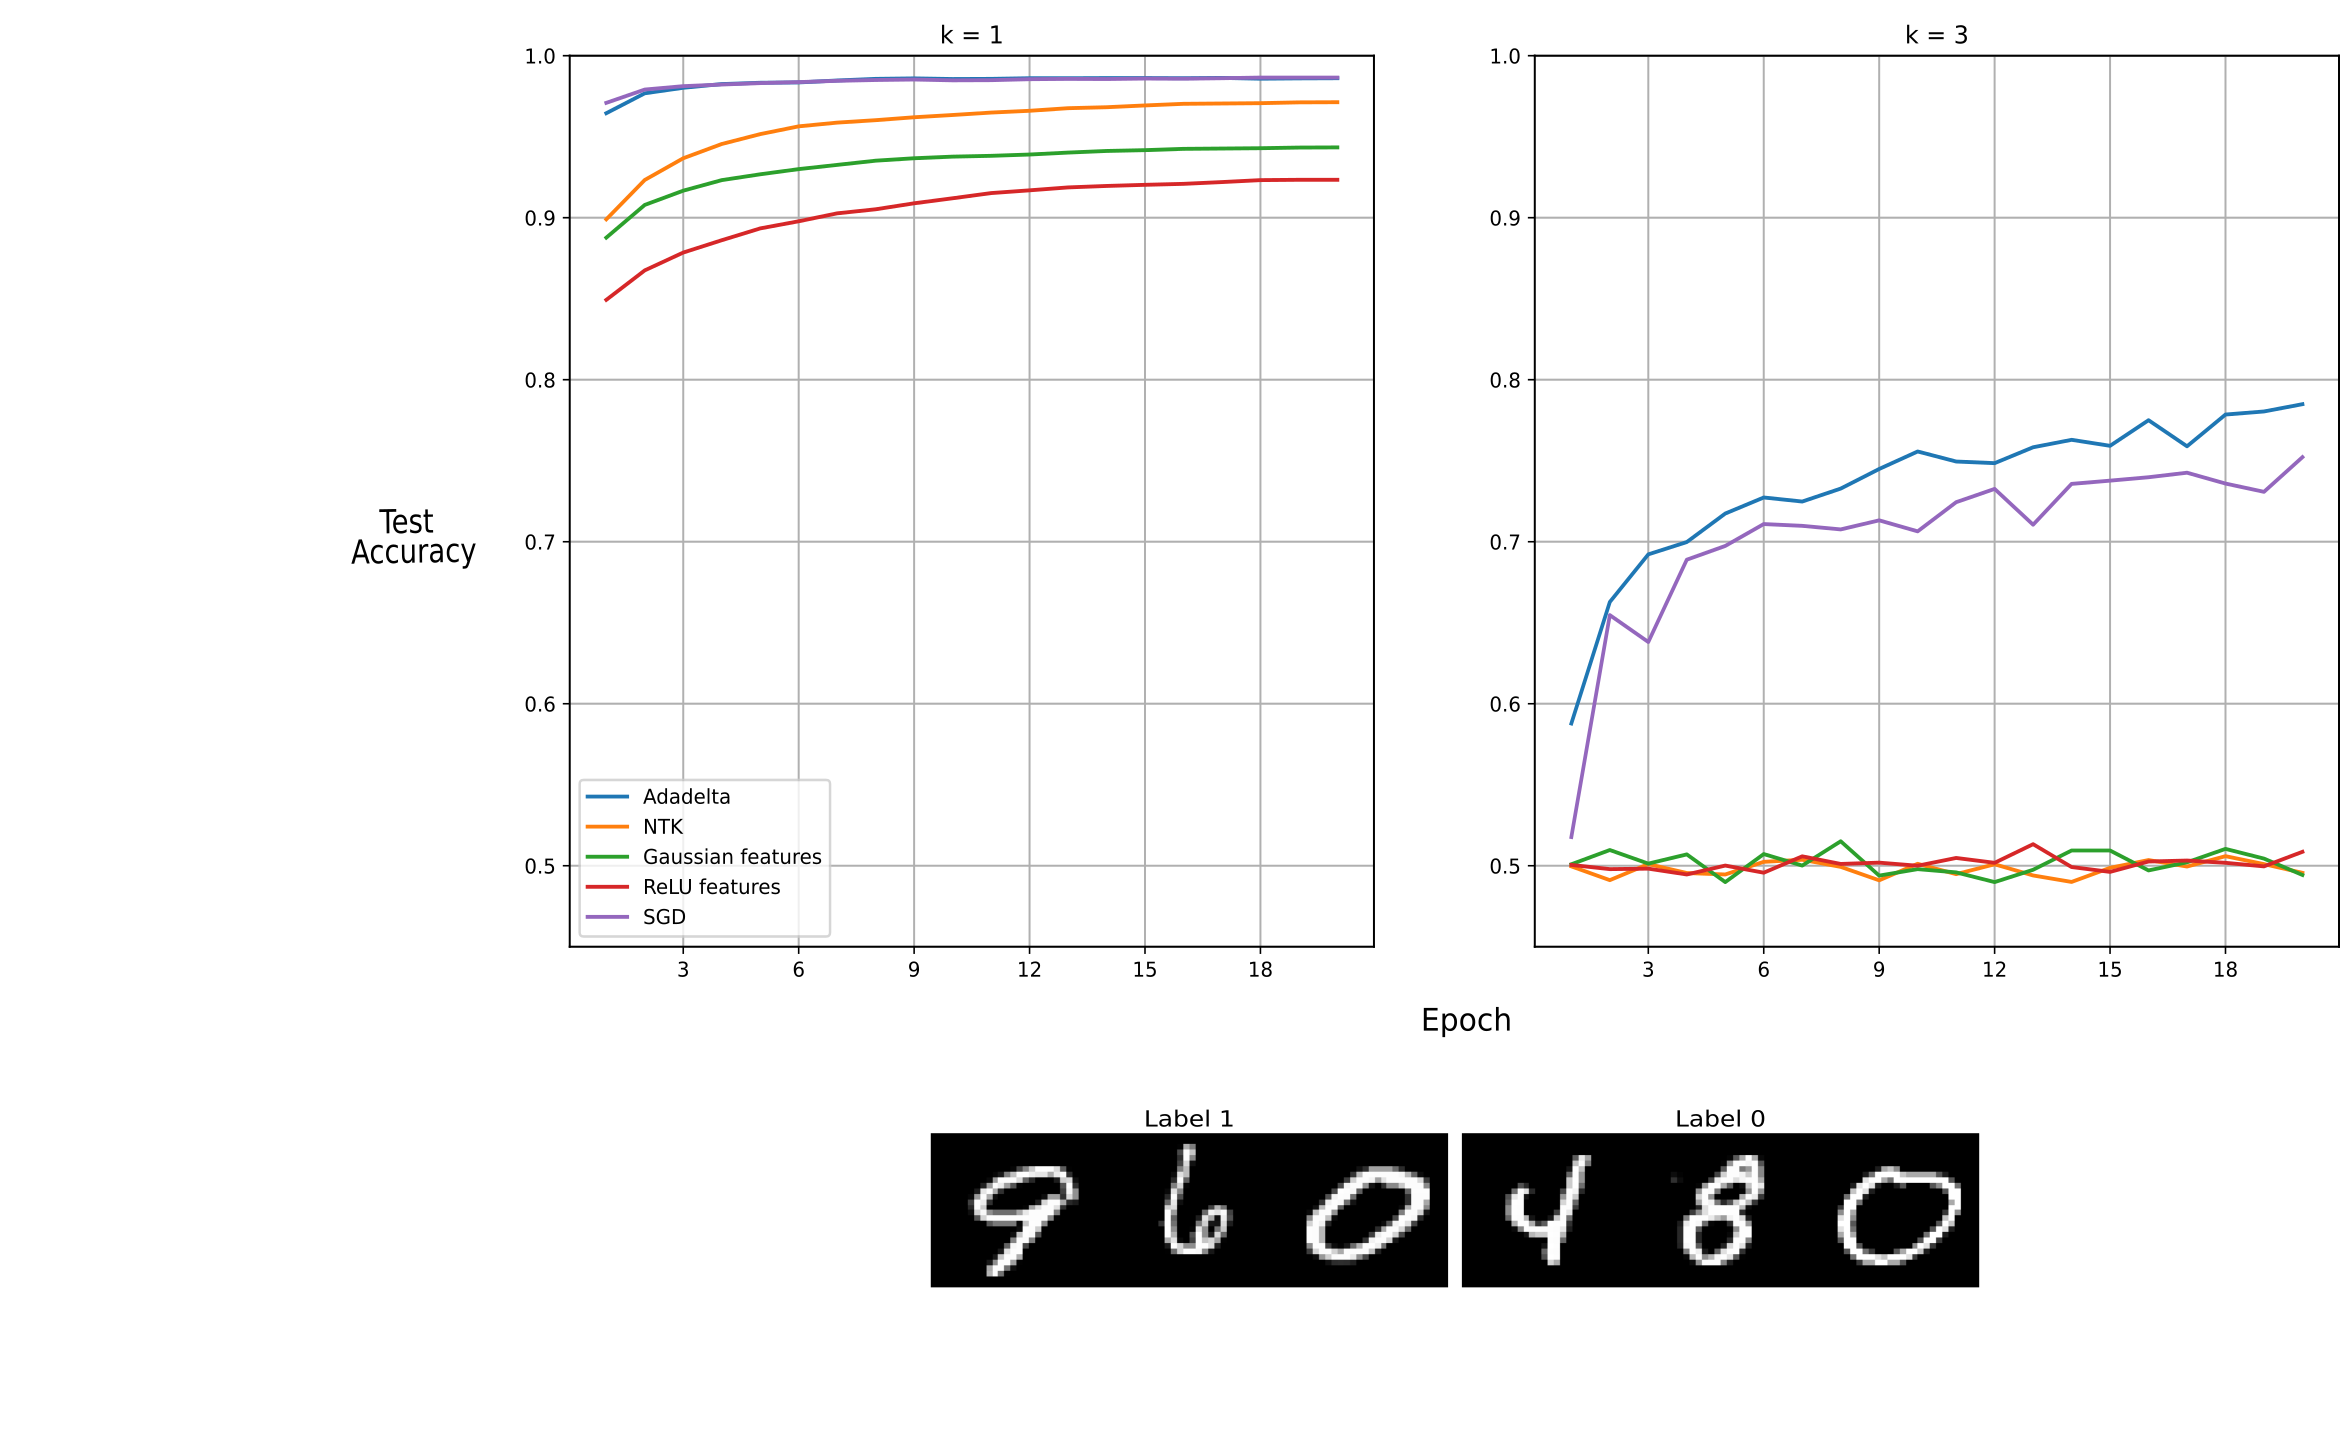
\includegraphics[width=1\linewidth]{figures/reproduce} 

}

\caption{Reproduced MNIST parity experiment result from \cite{DBLP:journals/corr/abs-2002-07400}}\label{fig:MNISTparity}
\end{figure}

\noindent The reproduced result can be observed in figure \ref{fig:MNISTparity} with example dataset. Similar to results from \cite{DBLP:journals/corr/abs-2002-07400}, all the methods succeed learning for \(k=1\) case. However, adadelta and SGD slightly outperformed lazy methods in this setting. In the case of \(k=3\), adadelta and SGD almost reach \(80\%\), but the performance of lazy methods doesn't go beyond a random guess.

\hypertarget{random-data}{%
\section{Random Data}\label{random-data}}

TODO: Write how this data generated, why it's interesting and why it is suitable for testing learning dynamics of the methods

\hypertarget{chap:chapter_3}{%
\chapter{Citations, cross-references, and collaboration}\label{chap:chapter_3}}

\chaptermark{Citations and cross-refs}

\minitoc 

\hypertarget{citations}{%
\section{Citations}\label{citations}}

The usual way to include citations in an \emph{R Markdown} document is to put references in a plain text file with the extension \textbf{.bib}, in \textbf{BibTex} format.\footnote{The bibliography can be in other formats as well, including EndNote (\textbf{.enl}) and RIS (\textbf{.ris}), see \href{https://rmarkdown.rstudio.com/authoring_bibliographies_and_citations.html}{rmarkdown.rstudio.com/authoring\_bibliographies\_and\_citations}.}
Then reference the path to this file in \textbf{index.Rmd}'s YAML header with \texttt{bibliography:\ example.bib}.

Most reference managers can create a .bib file with you references automatically.
However, the \textbf{by far} best reference manager to use with \emph{R Markdown} is \href{https://www.zotero.org}{Zotero} with the \href{https://retorque.re/zotero-better-bibtex/}{Better BibTex plug-in}, because the \texttt{citr} plugin for RStudio (see below) can read references directly from your Zotero library!

Here is an example of an entry in a \textbf{.bib} file:

\begin{Shaded}
\begin{Highlighting}[]
\VariableTok{@article}\NormalTok{\{}\OtherTok{Shea2014}\NormalTok{,}
  \DataTypeTok{author}\NormalTok{ =        \{Shea, Nicholas and Boldt, Annika\},}
  \DataTypeTok{journal}\NormalTok{ =       \{Trends in Cognitive Sciences\},}
  \DataTypeTok{pages}\NormalTok{ =         \{186--193\},}
  \DataTypeTok{title}\NormalTok{ =         \{\{Supra-personal cognitive control\}\},}
  \DataTypeTok{volume}\NormalTok{ =        \{18\},}
  \DataTypeTok{year}\NormalTok{ =          \{2014\},}
  \DataTypeTok{doi}\NormalTok{ =           \{10.1016/j.tics.2014.01.006\},}
\NormalTok{\}}
\end{Highlighting}
\end{Shaded}

In this entry highlighed section, `Shea2014' is the \textbf{citation identifier}.
To default way to cite an entry in your text is with this syntax: \texttt{{[}@citation-identifier{]}}.

So I might cite some things \autocite{Shea2014,Lottridge2012}.

\hypertarget{pdf-output}{%
\subsection{PDF output}\label{pdf-output}}

In PDF output, the bibliography is handled by the OxThesis LaTeX template.
If you set \texttt{bib-humanities:\ true} in \textbf{index.Rmd}, then in-text references will be formatted as author-year; otherwise references will be shown as numbers.

If you choose author-year formatting, a number of variations on the citation syntax are useful to know:

\begin{itemize}
\tightlist
\item
  Put author names outside the parenthesis

  \begin{itemize}
  \tightlist
  \item
    This: \texttt{@Shea2014\ says\ blah.}
  \item
    Becomes: \textcite{Shea2014} says blah.
  \end{itemize}
\item
  Include only the citation-year (in parenthesis)

  \begin{itemize}
  \tightlist
  \item
    This: \texttt{Shea\ et\ al.\ says\ blah\ {[}-@Shea2014{]}}
  \item
    Becomes: Shea et al.~says blah \autocite*{Shea2014}
  \end{itemize}
\item
  Add text and page or chapter references to the citation

  \begin{itemize}
  \tightlist
  \item
    This: \texttt{{[}see\ @Shea2014,\ pp.\ 33-35;\ also\ @Wu2016,\ ch.\ 1{]}}
  \item
    Becomes: Blah blah \autocites[see][pp.~33-35]{Shea2014}[also][ch.~1]{Wu2016}.
  \end{itemize}
\end{itemize}

\hypertarget{gitbook-output}{%
\subsection{Gitbook output}\label{gitbook-output}}

In gitbook output, citations are by default inserted in the Chicago author-date format.

To change the format, add \texttt{csl:\ some-other-style.csl} in \textbf{index.Rmd}'s YAML header.
You can browse through and download styles at \href{https://www.zotero.org/styles}{zotero.org/styles}.

\clearpage

\hypertarget{insert-references-easily-with-the-citr-add-in}{%
\subsection{\texorpdfstring{Insert references easily with the \texttt{citr} add-in}{Insert references easily with the citr add-in}}\label{insert-references-easily-with-the-citr-add-in}}

For an easy way to insert citations, try the \href{https://github.com/crsh/citr}{\texttt{citr}} RStudio add-in (Figure \ref{fig:citr}).
You can install this add-in by typing \texttt{install.packages("citr")} in the R Console.

\begin{figure}

{\centering 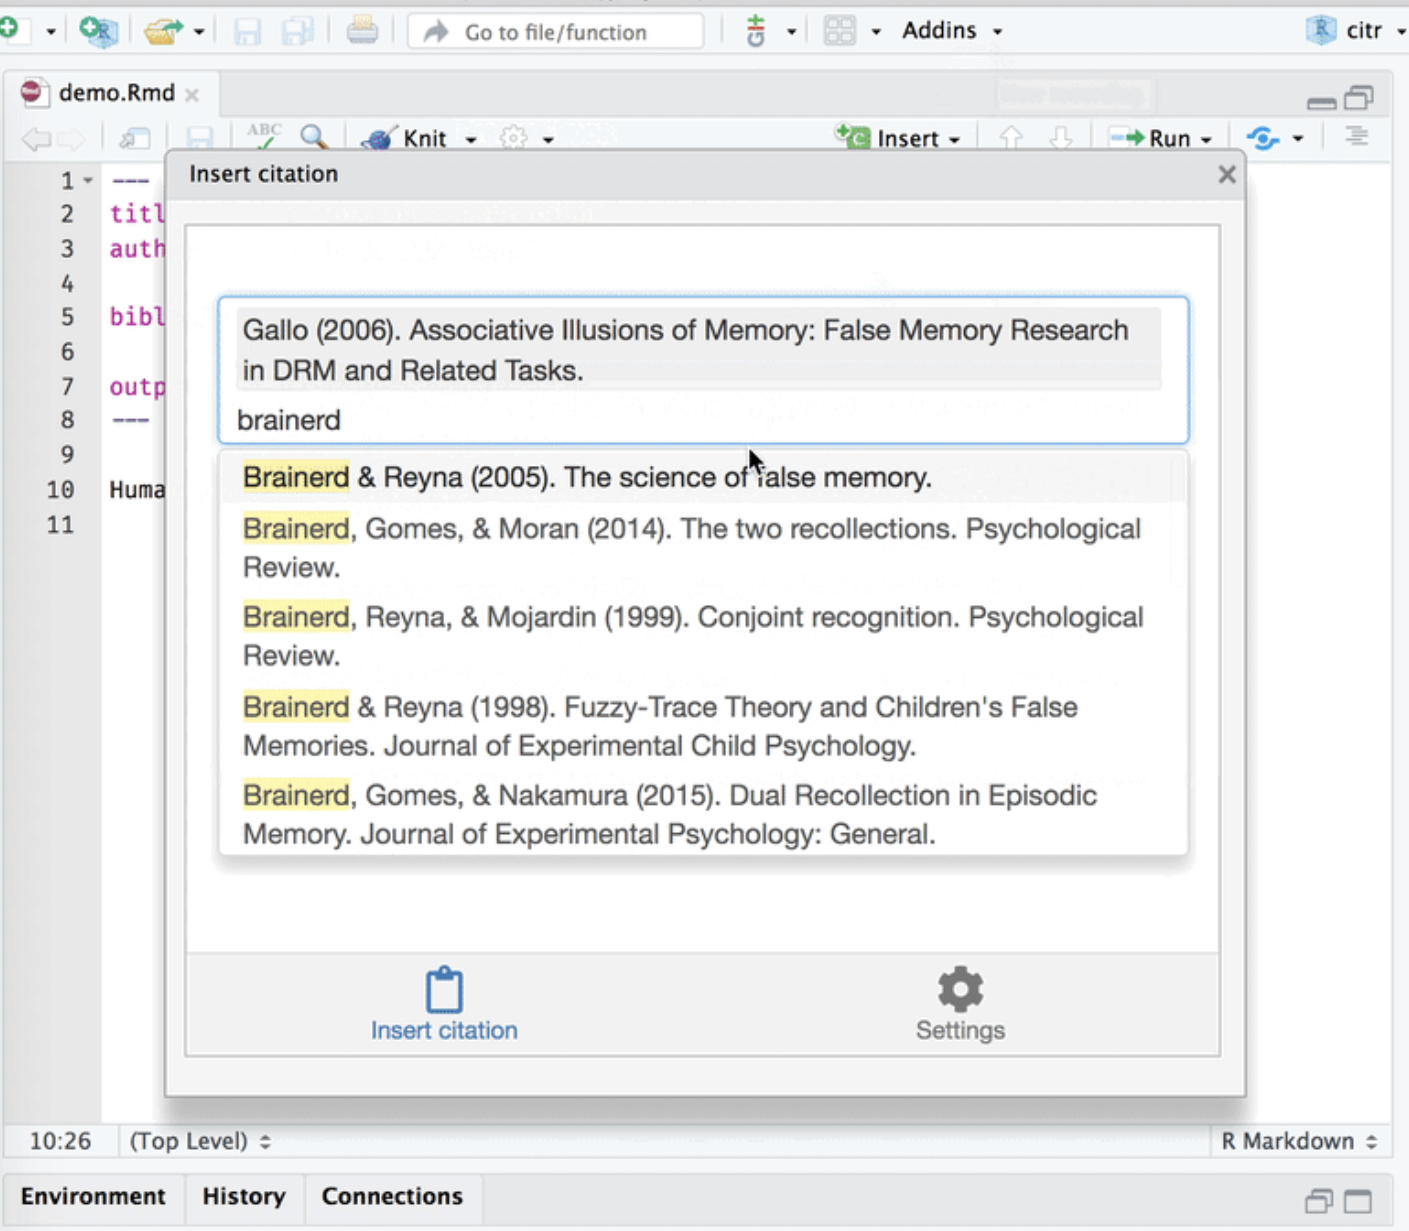
\includegraphics[width=0.8\linewidth]{figures/sample-content/citr} 

}

\caption{The `citr` add-in}\label{fig:citr}
\end{figure}

\hypertarget{cross-referencing}{%
\section{Cross-referencing}\label{cross-referencing}}

We can make cross-references to \textbf{sections} within our document, as well as to \textbf{figures} (images and plots) and \textbf{tables}.

The general cross-referencing syntax is \textbf{\texttt{\textbackslash{}@ref(label)}}

\hypertarget{section-references}{%
\subsection{Section references}\label{section-references}}

Headers are automatically assigned a reference label, which is the text in lower caps separated by dashes. For example, \texttt{\#\ My\ header} is automatically given the label \texttt{my-header}. So \texttt{\#\ My\ header} can be referenced with \texttt{\textbackslash{}@ref(my-section)}

Remember what we wrote in section \ref{citations}?

We can also use \textbf{hyperlink syntax} and add \# before the label, though this is only guaranteed to work properly in HTML output:

\begin{itemize}
\tightlist
\item
  So if we write \texttt{Remember\ what\ we\ wrote\ up\ in\ {[}the\ previous\ section{]}(\#citations)?}
\item
  It becomes Remember what we wrote up in \protect\hyperlink{citations}{the previous section}?
\end{itemize}

\hypertarget{creating-custom-labels}{%
\subsubsection{Creating custom labels}\label{creating-custom-labels}}

It is a very good idea to create \textbf{custom labels} for our sections. This is because the automatically assigned labels will change when we change the titles of the sections - to avoid this, we can create the labels ourselves and leave them untouched if we change the section titles.

We create custom labels by adding \texttt{\{\#label\}} after a header, e.g.~\texttt{\#\ My\ section\ \{\#my-label\}}.
See \protect\hyperlink{cites-and-refs}{our chapter title} for an example. That was section \ref{cites-and-refs}.

\hypertarget{figure-image-and-plot-references}{%
\subsection{Figure (image and plot) references}\label{figure-image-and-plot-references}}

\begin{itemize}
\tightlist
\item
  To refer to figures (i.e.~images and plots) use the syntax \texttt{\textbackslash{}@ref(fig:label)}
\item
  \textbf{GOTCHA}: Figures and tables must have captions if you wish to cross-reference them.
\end{itemize}

Let's add an image:

\begin{Shaded}
\begin{Highlighting}[]
\NormalTok{knitr}\OperatorTok{::}\KeywordTok{include_graphics}\NormalTok{(}\StringTok{"figures/sample-content/captain.jpeg"}\NormalTok{)}
\end{Highlighting}
\end{Shaded}

\begin{figure}

{\centering 
\includegraphics[width=0.65\linewidth]{figures/sample-content/captain} 

}

\caption{A marvel-lous meme}\label{fig:captain}
\end{figure}

We refer to this image with \texttt{\textbackslash{}@ref(fig:captain)}.
So Figure \ref{fig:captain} is \protect\hyperlink{fig:captain}{this image}.

And in Figure \ref{fig:cars-plot} we saw a \protect\hyperlink{fig:cars-plot}{cars plot}.

\hypertarget{table-references}{%
\subsection{Table references}\label{table-references}}

\begin{itemize}
\tightlist
\item
  To refer to tables use the syntax \texttt{\textbackslash{}@ref(tab:label)}
\end{itemize}

Let's include a table:

\begin{Shaded}
\begin{Highlighting}[]
\NormalTok{knitr}\OperatorTok{::}\KeywordTok{kable}\NormalTok{(cars[}\DecValTok{1}\OperatorTok{:}\DecValTok{5}\NormalTok{,],}
            \DataTypeTok{caption=}\StringTok{"Stopping cars"}\NormalTok{)}
\end{Highlighting}
\end{Shaded}

\begin{table}

\caption{\label{tab:cars-table2}Stopping cars}
\centering
\begin{tabular}[t]{r|r}
\hline
speed & dist\\
\hline
4 & 2\\
\hline
4 & 10\\
\hline
7 & 4\\
\hline
7 & 22\\
\hline
8 & 16\\
\hline
\end{tabular}
\end{table}

We refer to this table with \texttt{\textbackslash{}@ref(tab:cars-table2)}.
So Table \ref{tab:cars-table2} is \protect\hyperlink{tab:cars-table2}{this table}.

And in Table \ref{tab:cars-table} we saw more or less \protect\hyperlink{tab:cars-table}{the same cars table}.

\hypertarget{including-page-numbers}{%
\subsection{Including page numbers}\label{including-page-numbers}}

Finally, in the PDF output we might also want to include the page number of a reference, so that it's easy to find in physical printed output.
LaTeX has a command for this, which looks like this: \texttt{\textbackslash{}pageref\{fig/tab:label\}} (note: curly braces, not parentheses)

When we output to PDF, we can use raw LaTeX directly in our .Rmd files. So if we wanted to include the page of the cars plot we could write:

\begin{itemize}
\tightlist
\item
  This: \texttt{Figure\ \textbackslash{}@ref(fig:cars-plot)\ on\ page\ \textbackslash{}pageref(fig:cars-plot)}
\item
  Becomes: Figure \ref{fig:cars-plot} on page \pageref{fig:cars-plot}
\end{itemize}

\hypertarget{include-page-numbers-only-in-pdf-output}{%
\subsubsection{Include page numbers only in PDF output}\label{include-page-numbers-only-in-pdf-output}}

A problem here is that LaTeX commands don't display in HTML output, so in the gitbook output we'd see simply ``Figure \ref{fig:cars-plot} on page''.

One way to get around this is to use inline R code to insert the text, and use an \texttt{ifelse} statement to check the output format and then insert the appropriate text.

\begin{itemize}
\tightlist
\item
  So this: \texttt{\textasciigrave{}r\ ifelse(knitr::is\_latex\_output(),\ "Figure\ \textbackslash{}\textbackslash{}@ref(fig:cars-plot)\ on\ page\ \textbackslash{}\textbackslash{}pageref\{fig:cars-plot\}",\ "")\textasciigrave{}}
\item
  Inserts this (check this on both PDF and gitbook): Figure \ref{fig:cars-plot} on page \pageref{fig:cars-plot}
\end{itemize}

Note that we need to escape the backslash with another backslash here to get the correct output.

\hypertarget{collaborative-writing}{%
\section{Collaborative writing}\label{collaborative-writing}}

Best practices for collaboration and change tracking when using R Markdown are still an open question.
In the blog post \href{https://livefreeordichotomize.com/2018/09/14/one-year-to-dissertate/}{\textbf{One year to dissertate}} by Lucy D'Agostino, which I highly recommend, the author notes that she knits .Rmd files to a word document, then uses the \texttt{googledrive} R package to send this to Google Drive for comments / revisions from co-authors, then incorporates Google Drive suggestions \emph{by hand} into the .Rmd source files.
This is a bit clunky, and there are ongoing discussions among the \emph{R Markdown} developers about what the best way is to handle collaborative writing (see \href{https://github.com/rstudio/rmarkdown/issues/1463}{issue \#1463} on GitHub, where \href{http://criticmarkup.com}{CriticMarkup} is among the suggestions).

For now, this is an open question in the community of R Markdown users.
I often knit to a format that can easily be imported to Google Docs for comments, then go over suggested revisions and manually incorporate them back in to the .Rmd source files.
For articles, I sometimes upload a near-final draft to \href{https://www.overleaf.com/}{Overleaf}, then collaboratively make final edits to the LaTeX file there.
I suspect some great solution will be developed in the not-to-distant future, probably by the RStudio team.

\hypertarget{additional-resources}{%
\section{Additional resources}\label{additional-resources}}

\begin{itemize}
\item
  \emph{R Markdown: The Definitive Guide} - \url{https://bookdown.org/yihui/rmarkdown/}
\item
  \emph{R for Data Science} - \url{https://r4ds.had.co.nz}
\end{itemize}

\hypertarget{chap:chapter_4}{%
\chapter{Tables}\label{chap:chapter_4}}

\minitoc 

\hypertarget{making-latex-tables-play-nice}{%
\section{Making LaTeX tables play nice}\label{making-latex-tables-play-nice}}

Dealing with tables in LaTeX can be painful.
This section explains the main tricks you need to make the pain go away.

(Note: if you are looking at the ebook version, you will not see much difference in this section, as it is only relevant for PDF output!)

\hypertarget{making-your-table-pretty}{%
\subsection{Making your table pretty}\label{making-your-table-pretty}}

When you use \texttt{kable} to create tables, you will almost certainly want to set the option \texttt{booktabs\ =\ TRUE}.
This makes your table look a million times better:

\begin{Shaded}
\begin{Highlighting}[]
\KeywordTok{library}\NormalTok{(knitr)}
\KeywordTok{library}\NormalTok{(tidyverse)}

\KeywordTok{head}\NormalTok{(mtcars) }\OperatorTok\StringTok{ }
\StringTok{  }\KeywordTok{kable}\NormalTok{(}\DataTypeTok{booktabs =} \OtherTok{TRUE}\NormalTok{)}
\end{Highlighting}
\end{Shaded}

\begin{tabular}{lrrrrrrrrrrr}
\toprule
  & mpg & cyl & disp & hp & drat & wt & qsec & vs & am & gear & carb\\
\midrule
Mazda RX4 & 21.0 & 6 & 160 & 110 & 3.90 & 2.620 & 16.46 & 0 & 1 & 4 & 4\\
Mazda RX4 Wag & 21.0 & 6 & 160 & 110 & 3.90 & 2.875 & 17.02 & 0 & 1 & 4 & 4\\
Datsun 710 & 22.8 & 4 & 108 & 93 & 3.85 & 2.320 & 18.61 & 1 & 1 & 4 & 1\\
Hornet 4 Drive & 21.4 & 6 & 258 & 110 & 3.08 & 3.215 & 19.44 & 1 & 0 & 3 & 1\\
Hornet Sportabout & 18.7 & 8 & 360 & 175 & 3.15 & 3.440 & 17.02 & 0 & 0 & 3 & 2\\
\addlinespace
Valiant & 18.1 & 6 & 225 & 105 & 2.76 & 3.460 & 20.22 & 1 & 0 & 3 & 1\\
\bottomrule
\end{tabular}

\vspace{4mm}

Compare this to the default style, which looks terrible:

\begin{Shaded}
\begin{Highlighting}[]
\KeywordTok{head}\NormalTok{(mtcars) }\OperatorTok\StringTok{ }
\StringTok{  }\KeywordTok{kable}\NormalTok{()}
\end{Highlighting}
\end{Shaded}

\begin{tabular}{l|r|r|r|r|r|r|r|r|r|r|r}
\hline
  & mpg & cyl & disp & hp & drat & wt & qsec & vs & am & gear & carb\\
\hline
Mazda RX4 & 21.0 & 6 & 160 & 110 & 3.90 & 2.620 & 16.46 & 0 & 1 & 4 & 4\\
\hline
Mazda RX4 Wag & 21.0 & 6 & 160 & 110 & 3.90 & 2.875 & 17.02 & 0 & 1 & 4 & 4\\
\hline
Datsun 710 & 22.8 & 4 & 108 & 93 & 3.85 & 2.320 & 18.61 & 1 & 1 & 4 & 1\\
\hline
Hornet 4 Drive & 21.4 & 6 & 258 & 110 & 3.08 & 3.215 & 19.44 & 1 & 0 & 3 & 1\\
\hline
Hornet Sportabout & 18.7 & 8 & 360 & 175 & 3.15 & 3.440 & 17.02 & 0 & 0 & 3 & 2\\
\hline
Valiant & 18.1 & 6 & 225 & 105 & 2.76 & 3.460 & 20.22 & 1 & 0 & 3 & 1\\
\hline
\end{tabular}

\hypertarget{if-your-table-is-too-wide}{%
\subsection{If your table is too wide}\label{if-your-table-is-too-wide}}

You might find that your table expands into the margins of the page, like the tables above.
Fix this with the \texttt{kable\_styling} function from the \href{https://haozhu233.github.io/kableExtra/}{\texttt{kableExtra}} package:

\begin{Shaded}
\begin{Highlighting}[]
\KeywordTok{library}\NormalTok{(kableExtra)}

\KeywordTok{head}\NormalTok{(mtcars) }\OperatorTok\StringTok{ }
\StringTok{  }\KeywordTok{kable}\NormalTok{(}\DataTypeTok{booktabs =} \OtherTok{TRUE}\NormalTok{) }\OperatorTok\StringTok{ }
\StringTok{  }\KeywordTok{kable_styling}\NormalTok{(}\DataTypeTok{latex_options =} \StringTok{"scale_down"}\NormalTok{)}
\end{Highlighting}
\end{Shaded}

\begin{table}
\centering
\resizebox{\linewidth}{!}{
\begin{tabular}{lrrrrrrrrrrr}
\toprule
  & mpg & cyl & disp & hp & drat & wt & qsec & vs & am & gear & carb\\
\midrule
Mazda RX4 & 21.0 & 6 & 160 & 110 & 3.90 & 2.620 & 16.46 & 0 & 1 & 4 & 4\\
Mazda RX4 Wag & 21.0 & 6 & 160 & 110 & 3.90 & 2.875 & 17.02 & 0 & 1 & 4 & 4\\
Datsun 710 & 22.8 & 4 & 108 & 93 & 3.85 & 2.320 & 18.61 & 1 & 1 & 4 & 1\\
Hornet 4 Drive & 21.4 & 6 & 258 & 110 & 3.08 & 3.215 & 19.44 & 1 & 0 & 3 & 1\\
Hornet Sportabout & 18.7 & 8 & 360 & 175 & 3.15 & 3.440 & 17.02 & 0 & 0 & 3 & 2\\
\addlinespace
Valiant & 18.1 & 6 & 225 & 105 & 2.76 & 3.460 & 20.22 & 1 & 0 & 3 & 1\\
\bottomrule
\end{tabular}}
\end{table}

This scales down the table to fit the page width.

\hypertarget{if-your-table-is-too-long}{%
\subsection{If your table is too long}\label{if-your-table-is-too-long}}

If your table is too long to fit on a single page, set \texttt{longtable\ =\ TRUE} in the \texttt{kable} function to split the table across multiple pages.

\begin{Shaded}
\begin{Highlighting}[]
\NormalTok{a_long_table <-}\StringTok{ }\KeywordTok{rbind}\NormalTok{(mtcars, mtcars)}

\NormalTok{a_long_table }\OperatorTok\StringTok{ }
\StringTok{  }\KeywordTok{select}\NormalTok{(}\DecValTok{1}\OperatorTok{:}\DecValTok{8}\NormalTok{) }\OperatorTok\StringTok{ }
\StringTok{  }\KeywordTok{kable}\NormalTok{(}\DataTypeTok{booktabs =} \OtherTok{TRUE}\NormalTok{, }\DataTypeTok{longtable =} \OtherTok{TRUE}\NormalTok{)}
\end{Highlighting}
\end{Shaded}

\begin{longtable}{lrrrrrrrr}
\toprule
  & mpg & cyl & disp & hp & drat & wt & qsec & vs\\
\midrule
Mazda RX4 & 21.0 & 6 & 160.0 & 110 & 3.90 & 2.620 & 16.46 & 0\\
Mazda RX4 Wag & 21.0 & 6 & 160.0 & 110 & 3.90 & 2.875 & 17.02 & 0\\
Datsun 710 & 22.8 & 4 & 108.0 & 93 & 3.85 & 2.320 & 18.61 & 1\\
Hornet 4 Drive & 21.4 & 6 & 258.0 & 110 & 3.08 & 3.215 & 19.44 & 1\\
Hornet Sportabout & 18.7 & 8 & 360.0 & 175 & 3.15 & 3.440 & 17.02 & 0\\
\addlinespace
Valiant & 18.1 & 6 & 225.0 & 105 & 2.76 & 3.460 & 20.22 & 1\\
Duster 360 & 14.3 & 8 & 360.0 & 245 & 3.21 & 3.570 & 15.84 & 0\\
Merc 240D & 24.4 & 4 & 146.7 & 62 & 3.69 & 3.190 & 20.00 & 1\\
Merc 230 & 22.8 & 4 & 140.8 & 95 & 3.92 & 3.150 & 22.90 & 1\\
Merc 280 & 19.2 & 6 & 167.6 & 123 & 3.92 & 3.440 & 18.30 & 1\\
\addlinespace
Merc 280C & 17.8 & 6 & 167.6 & 123 & 3.92 & 3.440 & 18.90 & 1\\
Merc 450SE & 16.4 & 8 & 275.8 & 180 & 3.07 & 4.070 & 17.40 & 0\\
Merc 450SL & 17.3 & 8 & 275.8 & 180 & 3.07 & 3.730 & 17.60 & 0\\
Merc 450SLC & 15.2 & 8 & 275.8 & 180 & 3.07 & 3.780 & 18.00 & 0\\
Cadillac Fleetwood & 10.4 & 8 & 472.0 & 205 & 2.93 & 5.250 & 17.98 & 0\\
\addlinespace
Lincoln Continental & 10.4 & 8 & 460.0 & 215 & 3.00 & 5.424 & 17.82 & 0\\
Chrysler Imperial & 14.7 & 8 & 440.0 & 230 & 3.23 & 5.345 & 17.42 & 0\\
Fiat 128 & 32.4 & 4 & 78.7 & 66 & 4.08 & 2.200 & 19.47 & 1\\
Honda Civic & 30.4 & 4 & 75.7 & 52 & 4.93 & 1.615 & 18.52 & 1\\
Toyota Corolla & 33.9 & 4 & 71.1 & 65 & 4.22 & 1.835 & 19.90 & 1\\
\addlinespace
Toyota Corona & 21.5 & 4 & 120.1 & 97 & 3.70 & 2.465 & 20.01 & 1\\
Dodge Challenger & 15.5 & 8 & 318.0 & 150 & 2.76 & 3.520 & 16.87 & 0\\
AMC Javelin & 15.2 & 8 & 304.0 & 150 & 3.15 & 3.435 & 17.30 & 0\\
Camaro Z28 & 13.3 & 8 & 350.0 & 245 & 3.73 & 3.840 & 15.41 & 0\\
Pontiac Firebird & 19.2 & 8 & 400.0 & 175 & 3.08 & 3.845 & 17.05 & 0\\
\addlinespace
Fiat X1-9 & 27.3 & 4 & 79.0 & 66 & 4.08 & 1.935 & 18.90 & 1\\
Porsche 914-2 & 26.0 & 4 & 120.3 & 91 & 4.43 & 2.140 & 16.70 & 0\\
Lotus Europa & 30.4 & 4 & 95.1 & 113 & 3.77 & 1.513 & 16.90 & 1\\
Ford Pantera L & 15.8 & 8 & 351.0 & 264 & 4.22 & 3.170 & 14.50 & 0\\
Ferrari Dino & 19.7 & 6 & 145.0 & 175 & 3.62 & 2.770 & 15.50 & 0\\
\addlinespace
Maserati Bora & 15.0 & 8 & 301.0 & 335 & 3.54 & 3.570 & 14.60 & 0\\
Volvo 142E & 21.4 & 4 & 121.0 & 109 & 4.11 & 2.780 & 18.60 & 1\\
Mazda RX41 & 21.0 & 6 & 160.0 & 110 & 3.90 & 2.620 & 16.46 & 0\\
Mazda RX4 Wag1 & 21.0 & 6 & 160.0 & 110 & 3.90 & 2.875 & 17.02 & 0\\
Datsun 7101 & 22.8 & 4 & 108.0 & 93 & 3.85 & 2.320 & 18.61 & 1\\
\addlinespace
Hornet 4 Drive1 & 21.4 & 6 & 258.0 & 110 & 3.08 & 3.215 & 19.44 & 1\\
Hornet Sportabout1 & 18.7 & 8 & 360.0 & 175 & 3.15 & 3.440 & 17.02 & 0\\
Valiant1 & 18.1 & 6 & 225.0 & 105 & 2.76 & 3.460 & 20.22 & 1\\
Duster 3601 & 14.3 & 8 & 360.0 & 245 & 3.21 & 3.570 & 15.84 & 0\\
Merc 240D1 & 24.4 & 4 & 146.7 & 62 & 3.69 & 3.190 & 20.00 & 1\\
\addlinespace
Merc 2301 & 22.8 & 4 & 140.8 & 95 & 3.92 & 3.150 & 22.90 & 1\\
Merc 2801 & 19.2 & 6 & 167.6 & 123 & 3.92 & 3.440 & 18.30 & 1\\
Merc 280C1 & 17.8 & 6 & 167.6 & 123 & 3.92 & 3.440 & 18.90 & 1\\
Merc 450SE1 & 16.4 & 8 & 275.8 & 180 & 3.07 & 4.070 & 17.40 & 0\\
Merc 450SL1 & 17.3 & 8 & 275.8 & 180 & 3.07 & 3.730 & 17.60 & 0\\
\addlinespace
Merc 450SLC1 & 15.2 & 8 & 275.8 & 180 & 3.07 & 3.780 & 18.00 & 0\\
Cadillac Fleetwood1 & 10.4 & 8 & 472.0 & 205 & 2.93 & 5.250 & 17.98 & 0\\
Lincoln Continental1 & 10.4 & 8 & 460.0 & 215 & 3.00 & 5.424 & 17.82 & 0\\
Chrysler Imperial1 & 14.7 & 8 & 440.0 & 230 & 3.23 & 5.345 & 17.42 & 0\\
Fiat 1281 & 32.4 & 4 & 78.7 & 66 & 4.08 & 2.200 & 19.47 & 1\\
\addlinespace
Honda Civic1 & 30.4 & 4 & 75.7 & 52 & 4.93 & 1.615 & 18.52 & 1\\
Toyota Corolla1 & 33.9 & 4 & 71.1 & 65 & 4.22 & 1.835 & 19.90 & 1\\
Toyota Corona1 & 21.5 & 4 & 120.1 & 97 & 3.70 & 2.465 & 20.01 & 1\\
Dodge Challenger1 & 15.5 & 8 & 318.0 & 150 & 2.76 & 3.520 & 16.87 & 0\\
AMC Javelin1 & 15.2 & 8 & 304.0 & 150 & 3.15 & 3.435 & 17.30 & 0\\
\addlinespace
Camaro Z281 & 13.3 & 8 & 350.0 & 245 & 3.73 & 3.840 & 15.41 & 0\\
Pontiac Firebird1 & 19.2 & 8 & 400.0 & 175 & 3.08 & 3.845 & 17.05 & 0\\
Fiat X1-91 & 27.3 & 4 & 79.0 & 66 & 4.08 & 1.935 & 18.90 & 1\\
Porsche 914-21 & 26.0 & 4 & 120.3 & 91 & 4.43 & 2.140 & 16.70 & 0\\
Lotus Europa1 & 30.4 & 4 & 95.1 & 113 & 3.77 & 1.513 & 16.90 & 1\\
\addlinespace
Ford Pantera L1 & 15.8 & 8 & 351.0 & 264 & 4.22 & 3.170 & 14.50 & 0\\
Ferrari Dino1 & 19.7 & 6 & 145.0 & 175 & 3.62 & 2.770 & 15.50 & 0\\
Maserati Bora1 & 15.0 & 8 & 301.0 & 335 & 3.54 & 3.570 & 14.60 & 0\\
Volvo 142E1 & 21.4 & 4 & 121.0 & 109 & 4.11 & 2.780 & 18.60 & 1\\
\bottomrule
\end{longtable}

When you do this, you'll probably want to make the header repeat on new pages.
Do this with the \texttt{kable\_styling} function from \texttt{kableExtra}:

\begin{Shaded}
\begin{Highlighting}[]
\NormalTok{a_long_table }\OperatorTok\StringTok{ }
\StringTok{  }\KeywordTok{kable}\NormalTok{(}\DataTypeTok{booktabs =} \OtherTok{TRUE}\NormalTok{, }\DataTypeTok{longtable =} \OtherTok{TRUE}\NormalTok{) }\OperatorTok\StringTok{ }
\StringTok{  }\KeywordTok{kable_styling}\NormalTok{(}\DataTypeTok{latex_options =} \StringTok{"repeat_header"}\NormalTok{)}
\end{Highlighting}
\end{Shaded}

\begin{longtable}{lrrrrrrrrrrr}
\toprule
  & mpg & cyl & disp & hp & drat & wt & qsec & vs & am & gear & carb\\
\midrule
\endfirsthead
\multicolumn{12}{@{}l}{\textit{(continued)}}\\
\toprule
  & mpg & cyl & disp & hp & drat & wt & qsec & vs & am & gear & carb\\
\midrule
\endhead

\endfoot
\bottomrule
\endlastfoot
Mazda RX4 & 21.0 & 6 & 160.0 & 110 & 3.90 & 2.620 & 16.46 & 0 & 1 & 4 & 4\\
Mazda RX4 Wag & 21.0 & 6 & 160.0 & 110 & 3.90 & 2.875 & 17.02 & 0 & 1 & 4 & 4\\
Datsun 710 & 22.8 & 4 & 108.0 & 93 & 3.85 & 2.320 & 18.61 & 1 & 1 & 4 & 1\\
Hornet 4 Drive & 21.4 & 6 & 258.0 & 110 & 3.08 & 3.215 & 19.44 & 1 & 0 & 3 & 1\\
Hornet Sportabout & 18.7 & 8 & 360.0 & 175 & 3.15 & 3.440 & 17.02 & 0 & 0 & 3 & 2\\
\addlinespace
Valiant & 18.1 & 6 & 225.0 & 105 & 2.76 & 3.460 & 20.22 & 1 & 0 & 3 & 1\\
Duster 360 & 14.3 & 8 & 360.0 & 245 & 3.21 & 3.570 & 15.84 & 0 & 0 & 3 & 4\\
Merc 240D & 24.4 & 4 & 146.7 & 62 & 3.69 & 3.190 & 20.00 & 1 & 0 & 4 & 2\\
Merc 230 & 22.8 & 4 & 140.8 & 95 & 3.92 & 3.150 & 22.90 & 1 & 0 & 4 & 2\\
Merc 280 & 19.2 & 6 & 167.6 & 123 & 3.92 & 3.440 & 18.30 & 1 & 0 & 4 & 4\\
\addlinespace
Merc 280C & 17.8 & 6 & 167.6 & 123 & 3.92 & 3.440 & 18.90 & 1 & 0 & 4 & 4\\
Merc 450SE & 16.4 & 8 & 275.8 & 180 & 3.07 & 4.070 & 17.40 & 0 & 0 & 3 & 3\\
Merc 450SL & 17.3 & 8 & 275.8 & 180 & 3.07 & 3.730 & 17.60 & 0 & 0 & 3 & 3\\
Merc 450SLC & 15.2 & 8 & 275.8 & 180 & 3.07 & 3.780 & 18.00 & 0 & 0 & 3 & 3\\
Cadillac Fleetwood & 10.4 & 8 & 472.0 & 205 & 2.93 & 5.250 & 17.98 & 0 & 0 & 3 & 4\\
\addlinespace
Lincoln Continental & 10.4 & 8 & 460.0 & 215 & 3.00 & 5.424 & 17.82 & 0 & 0 & 3 & 4\\
Chrysler Imperial & 14.7 & 8 & 440.0 & 230 & 3.23 & 5.345 & 17.42 & 0 & 0 & 3 & 4\\
Fiat 128 & 32.4 & 4 & 78.7 & 66 & 4.08 & 2.200 & 19.47 & 1 & 1 & 4 & 1\\
Honda Civic & 30.4 & 4 & 75.7 & 52 & 4.93 & 1.615 & 18.52 & 1 & 1 & 4 & 2\\
Toyota Corolla & 33.9 & 4 & 71.1 & 65 & 4.22 & 1.835 & 19.90 & 1 & 1 & 4 & 1\\
\addlinespace
Toyota Corona & 21.5 & 4 & 120.1 & 97 & 3.70 & 2.465 & 20.01 & 1 & 0 & 3 & 1\\
Dodge Challenger & 15.5 & 8 & 318.0 & 150 & 2.76 & 3.520 & 16.87 & 0 & 0 & 3 & 2\\
AMC Javelin & 15.2 & 8 & 304.0 & 150 & 3.15 & 3.435 & 17.30 & 0 & 0 & 3 & 2\\
Camaro Z28 & 13.3 & 8 & 350.0 & 245 & 3.73 & 3.840 & 15.41 & 0 & 0 & 3 & 4\\
Pontiac Firebird & 19.2 & 8 & 400.0 & 175 & 3.08 & 3.845 & 17.05 & 0 & 0 & 3 & 2\\
\addlinespace
Fiat X1-9 & 27.3 & 4 & 79.0 & 66 & 4.08 & 1.935 & 18.90 & 1 & 1 & 4 & 1\\
Porsche 914-2 & 26.0 & 4 & 120.3 & 91 & 4.43 & 2.140 & 16.70 & 0 & 1 & 5 & 2\\
Lotus Europa & 30.4 & 4 & 95.1 & 113 & 3.77 & 1.513 & 16.90 & 1 & 1 & 5 & 2\\
Ford Pantera L & 15.8 & 8 & 351.0 & 264 & 4.22 & 3.170 & 14.50 & 0 & 1 & 5 & 4\\
Ferrari Dino & 19.7 & 6 & 145.0 & 175 & 3.62 & 2.770 & 15.50 & 0 & 1 & 5 & 6\\
\addlinespace
Maserati Bora & 15.0 & 8 & 301.0 & 335 & 3.54 & 3.570 & 14.60 & 0 & 1 & 5 & 8\\
Volvo 142E & 21.4 & 4 & 121.0 & 109 & 4.11 & 2.780 & 18.60 & 1 & 1 & 4 & 2\\
Mazda RX41 & 21.0 & 6 & 160.0 & 110 & 3.90 & 2.620 & 16.46 & 0 & 1 & 4 & 4\\
Mazda RX4 Wag1 & 21.0 & 6 & 160.0 & 110 & 3.90 & 2.875 & 17.02 & 0 & 1 & 4 & 4\\
Datsun 7101 & 22.8 & 4 & 108.0 & 93 & 3.85 & 2.320 & 18.61 & 1 & 1 & 4 & 1\\
\addlinespace
Hornet 4 Drive1 & 21.4 & 6 & 258.0 & 110 & 3.08 & 3.215 & 19.44 & 1 & 0 & 3 & 1\\
Hornet Sportabout1 & 18.7 & 8 & 360.0 & 175 & 3.15 & 3.440 & 17.02 & 0 & 0 & 3 & 2\\
Valiant1 & 18.1 & 6 & 225.0 & 105 & 2.76 & 3.460 & 20.22 & 1 & 0 & 3 & 1\\
Duster 3601 & 14.3 & 8 & 360.0 & 245 & 3.21 & 3.570 & 15.84 & 0 & 0 & 3 & 4\\
Merc 240D1 & 24.4 & 4 & 146.7 & 62 & 3.69 & 3.190 & 20.00 & 1 & 0 & 4 & 2\\
\addlinespace
Merc 2301 & 22.8 & 4 & 140.8 & 95 & 3.92 & 3.150 & 22.90 & 1 & 0 & 4 & 2\\
Merc 2801 & 19.2 & 6 & 167.6 & 123 & 3.92 & 3.440 & 18.30 & 1 & 0 & 4 & 4\\
Merc 280C1 & 17.8 & 6 & 167.6 & 123 & 3.92 & 3.440 & 18.90 & 1 & 0 & 4 & 4\\
Merc 450SE1 & 16.4 & 8 & 275.8 & 180 & 3.07 & 4.070 & 17.40 & 0 & 0 & 3 & 3\\
Merc 450SL1 & 17.3 & 8 & 275.8 & 180 & 3.07 & 3.730 & 17.60 & 0 & 0 & 3 & 3\\
\addlinespace
Merc 450SLC1 & 15.2 & 8 & 275.8 & 180 & 3.07 & 3.780 & 18.00 & 0 & 0 & 3 & 3\\
Cadillac Fleetwood1 & 10.4 & 8 & 472.0 & 205 & 2.93 & 5.250 & 17.98 & 0 & 0 & 3 & 4\\
Lincoln Continental1 & 10.4 & 8 & 460.0 & 215 & 3.00 & 5.424 & 17.82 & 0 & 0 & 3 & 4\\
Chrysler Imperial1 & 14.7 & 8 & 440.0 & 230 & 3.23 & 5.345 & 17.42 & 0 & 0 & 3 & 4\\
Fiat 1281 & 32.4 & 4 & 78.7 & 66 & 4.08 & 2.200 & 19.47 & 1 & 1 & 4 & 1\\
\addlinespace
Honda Civic1 & 30.4 & 4 & 75.7 & 52 & 4.93 & 1.615 & 18.52 & 1 & 1 & 4 & 2\\
Toyota Corolla1 & 33.9 & 4 & 71.1 & 65 & 4.22 & 1.835 & 19.90 & 1 & 1 & 4 & 1\\
Toyota Corona1 & 21.5 & 4 & 120.1 & 97 & 3.70 & 2.465 & 20.01 & 1 & 0 & 3 & 1\\
Dodge Challenger1 & 15.5 & 8 & 318.0 & 150 & 2.76 & 3.520 & 16.87 & 0 & 0 & 3 & 2\\
AMC Javelin1 & 15.2 & 8 & 304.0 & 150 & 3.15 & 3.435 & 17.30 & 0 & 0 & 3 & 2\\
\addlinespace
Camaro Z281 & 13.3 & 8 & 350.0 & 245 & 3.73 & 3.840 & 15.41 & 0 & 0 & 3 & 4\\
Pontiac Firebird1 & 19.2 & 8 & 400.0 & 175 & 3.08 & 3.845 & 17.05 & 0 & 0 & 3 & 2\\
Fiat X1-91 & 27.3 & 4 & 79.0 & 66 & 4.08 & 1.935 & 18.90 & 1 & 1 & 4 & 1\\
Porsche 914-21 & 26.0 & 4 & 120.3 & 91 & 4.43 & 2.140 & 16.70 & 0 & 1 & 5 & 2\\
Lotus Europa1 & 30.4 & 4 & 95.1 & 113 & 3.77 & 1.513 & 16.90 & 1 & 1 & 5 & 2\\
\addlinespace
Ford Pantera L1 & 15.8 & 8 & 351.0 & 264 & 4.22 & 3.170 & 14.50 & 0 & 1 & 5 & 4\\
Ferrari Dino1 & 19.7 & 6 & 145.0 & 175 & 3.62 & 2.770 & 15.50 & 0 & 1 & 5 & 6\\
Maserati Bora1 & 15.0 & 8 & 301.0 & 335 & 3.54 & 3.570 & 14.60 & 0 & 1 & 5 & 8\\
Volvo 142E1 & 21.4 & 4 & 121.0 & 109 & 4.11 & 2.780 & 18.60 & 1 & 1 & 4 & 2\\*
\end{longtable}

Unfortunately, we cannot use the \texttt{scale\_down} option with a \texttt{longtable}.
So if a \texttt{longtable} is too wide, you can either manually adjust the font size, or show the table in landscape layout.
To adjust the font size, use kableExtra's \texttt{font\_size} option:

\begin{Shaded}
\begin{Highlighting}[]
\NormalTok{a_long_table }\OperatorTok\StringTok{ }
\StringTok{  }\KeywordTok{kable}\NormalTok{(}\DataTypeTok{booktabs =} \OtherTok{TRUE}\NormalTok{, }\DataTypeTok{longtable =} \OtherTok{TRUE}\NormalTok{) }\OperatorTok\StringTok{ }
\StringTok{  }\KeywordTok{kable_styling}\NormalTok{(}\DataTypeTok{font_size =} \DecValTok{9}\NormalTok{, }\DataTypeTok{latex_options =} \StringTok{"repeat_header"}\NormalTok{)}
\end{Highlighting}
\end{Shaded}

\begingroup\fontsize{9}{11}\selectfont

\begin{longtable}{lrrrrrrrrrrr}
\toprule
  & mpg & cyl & disp & hp & drat & wt & qsec & vs & am & gear & carb\\
\midrule
\endfirsthead
\multicolumn{12}{@{}l}{\textit{(continued)}}\\
\toprule
  & mpg & cyl & disp & hp & drat & wt & qsec & vs & am & gear & carb\\
\midrule
\endhead

\endfoot
\bottomrule
\endlastfoot
Mazda RX4 & 21.0 & 6 & 160.0 & 110 & 3.90 & 2.620 & 16.46 & 0 & 1 & 4 & 4\\
Mazda RX4 Wag & 21.0 & 6 & 160.0 & 110 & 3.90 & 2.875 & 17.02 & 0 & 1 & 4 & 4\\
Datsun 710 & 22.8 & 4 & 108.0 & 93 & 3.85 & 2.320 & 18.61 & 1 & 1 & 4 & 1\\
Hornet 4 Drive & 21.4 & 6 & 258.0 & 110 & 3.08 & 3.215 & 19.44 & 1 & 0 & 3 & 1\\
Hornet Sportabout & 18.7 & 8 & 360.0 & 175 & 3.15 & 3.440 & 17.02 & 0 & 0 & 3 & 2\\
\addlinespace
Valiant & 18.1 & 6 & 225.0 & 105 & 2.76 & 3.460 & 20.22 & 1 & 0 & 3 & 1\\
Duster 360 & 14.3 & 8 & 360.0 & 245 & 3.21 & 3.570 & 15.84 & 0 & 0 & 3 & 4\\
Merc 240D & 24.4 & 4 & 146.7 & 62 & 3.69 & 3.190 & 20.00 & 1 & 0 & 4 & 2\\
Merc 230 & 22.8 & 4 & 140.8 & 95 & 3.92 & 3.150 & 22.90 & 1 & 0 & 4 & 2\\
Merc 280 & 19.2 & 6 & 167.6 & 123 & 3.92 & 3.440 & 18.30 & 1 & 0 & 4 & 4\\
\addlinespace
Merc 280C & 17.8 & 6 & 167.6 & 123 & 3.92 & 3.440 & 18.90 & 1 & 0 & 4 & 4\\
Merc 450SE & 16.4 & 8 & 275.8 & 180 & 3.07 & 4.070 & 17.40 & 0 & 0 & 3 & 3\\
Merc 450SL & 17.3 & 8 & 275.8 & 180 & 3.07 & 3.730 & 17.60 & 0 & 0 & 3 & 3\\
Merc 450SLC & 15.2 & 8 & 275.8 & 180 & 3.07 & 3.780 & 18.00 & 0 & 0 & 3 & 3\\
Cadillac Fleetwood & 10.4 & 8 & 472.0 & 205 & 2.93 & 5.250 & 17.98 & 0 & 0 & 3 & 4\\
\addlinespace
Lincoln Continental & 10.4 & 8 & 460.0 & 215 & 3.00 & 5.424 & 17.82 & 0 & 0 & 3 & 4\\
Chrysler Imperial & 14.7 & 8 & 440.0 & 230 & 3.23 & 5.345 & 17.42 & 0 & 0 & 3 & 4\\
Fiat 128 & 32.4 & 4 & 78.7 & 66 & 4.08 & 2.200 & 19.47 & 1 & 1 & 4 & 1\\
Honda Civic & 30.4 & 4 & 75.7 & 52 & 4.93 & 1.615 & 18.52 & 1 & 1 & 4 & 2\\
Toyota Corolla & 33.9 & 4 & 71.1 & 65 & 4.22 & 1.835 & 19.90 & 1 & 1 & 4 & 1\\
\addlinespace
Toyota Corona & 21.5 & 4 & 120.1 & 97 & 3.70 & 2.465 & 20.01 & 1 & 0 & 3 & 1\\
Dodge Challenger & 15.5 & 8 & 318.0 & 150 & 2.76 & 3.520 & 16.87 & 0 & 0 & 3 & 2\\
AMC Javelin & 15.2 & 8 & 304.0 & 150 & 3.15 & 3.435 & 17.30 & 0 & 0 & 3 & 2\\
Camaro Z28 & 13.3 & 8 & 350.0 & 245 & 3.73 & 3.840 & 15.41 & 0 & 0 & 3 & 4\\
Pontiac Firebird & 19.2 & 8 & 400.0 & 175 & 3.08 & 3.845 & 17.05 & 0 & 0 & 3 & 2\\
\addlinespace
Fiat X1-9 & 27.3 & 4 & 79.0 & 66 & 4.08 & 1.935 & 18.90 & 1 & 1 & 4 & 1\\
Porsche 914-2 & 26.0 & 4 & 120.3 & 91 & 4.43 & 2.140 & 16.70 & 0 & 1 & 5 & 2\\
Lotus Europa & 30.4 & 4 & 95.1 & 113 & 3.77 & 1.513 & 16.90 & 1 & 1 & 5 & 2\\
Ford Pantera L & 15.8 & 8 & 351.0 & 264 & 4.22 & 3.170 & 14.50 & 0 & 1 & 5 & 4\\
Ferrari Dino & 19.7 & 6 & 145.0 & 175 & 3.62 & 2.770 & 15.50 & 0 & 1 & 5 & 6\\
\addlinespace
Maserati Bora & 15.0 & 8 & 301.0 & 335 & 3.54 & 3.570 & 14.60 & 0 & 1 & 5 & 8\\
Volvo 142E & 21.4 & 4 & 121.0 & 109 & 4.11 & 2.780 & 18.60 & 1 & 1 & 4 & 2\\
Mazda RX41 & 21.0 & 6 & 160.0 & 110 & 3.90 & 2.620 & 16.46 & 0 & 1 & 4 & 4\\
Mazda RX4 Wag1 & 21.0 & 6 & 160.0 & 110 & 3.90 & 2.875 & 17.02 & 0 & 1 & 4 & 4\\
Datsun 7101 & 22.8 & 4 & 108.0 & 93 & 3.85 & 2.320 & 18.61 & 1 & 1 & 4 & 1\\
\addlinespace
Hornet 4 Drive1 & 21.4 & 6 & 258.0 & 110 & 3.08 & 3.215 & 19.44 & 1 & 0 & 3 & 1\\
Hornet Sportabout1 & 18.7 & 8 & 360.0 & 175 & 3.15 & 3.440 & 17.02 & 0 & 0 & 3 & 2\\
Valiant1 & 18.1 & 6 & 225.0 & 105 & 2.76 & 3.460 & 20.22 & 1 & 0 & 3 & 1\\
Duster 3601 & 14.3 & 8 & 360.0 & 245 & 3.21 & 3.570 & 15.84 & 0 & 0 & 3 & 4\\
Merc 240D1 & 24.4 & 4 & 146.7 & 62 & 3.69 & 3.190 & 20.00 & 1 & 0 & 4 & 2\\
\addlinespace
Merc 2301 & 22.8 & 4 & 140.8 & 95 & 3.92 & 3.150 & 22.90 & 1 & 0 & 4 & 2\\
Merc 2801 & 19.2 & 6 & 167.6 & 123 & 3.92 & 3.440 & 18.30 & 1 & 0 & 4 & 4\\
Merc 280C1 & 17.8 & 6 & 167.6 & 123 & 3.92 & 3.440 & 18.90 & 1 & 0 & 4 & 4\\
Merc 450SE1 & 16.4 & 8 & 275.8 & 180 & 3.07 & 4.070 & 17.40 & 0 & 0 & 3 & 3\\
Merc 450SL1 & 17.3 & 8 & 275.8 & 180 & 3.07 & 3.730 & 17.60 & 0 & 0 & 3 & 3\\
\addlinespace
Merc 450SLC1 & 15.2 & 8 & 275.8 & 180 & 3.07 & 3.780 & 18.00 & 0 & 0 & 3 & 3\\
Cadillac Fleetwood1 & 10.4 & 8 & 472.0 & 205 & 2.93 & 5.250 & 17.98 & 0 & 0 & 3 & 4\\
Lincoln Continental1 & 10.4 & 8 & 460.0 & 215 & 3.00 & 5.424 & 17.82 & 0 & 0 & 3 & 4\\
Chrysler Imperial1 & 14.7 & 8 & 440.0 & 230 & 3.23 & 5.345 & 17.42 & 0 & 0 & 3 & 4\\
Fiat 1281 & 32.4 & 4 & 78.7 & 66 & 4.08 & 2.200 & 19.47 & 1 & 1 & 4 & 1\\
\addlinespace
Honda Civic1 & 30.4 & 4 & 75.7 & 52 & 4.93 & 1.615 & 18.52 & 1 & 1 & 4 & 2\\
Toyota Corolla1 & 33.9 & 4 & 71.1 & 65 & 4.22 & 1.835 & 19.90 & 1 & 1 & 4 & 1\\
Toyota Corona1 & 21.5 & 4 & 120.1 & 97 & 3.70 & 2.465 & 20.01 & 1 & 0 & 3 & 1\\
Dodge Challenger1 & 15.5 & 8 & 318.0 & 150 & 2.76 & 3.520 & 16.87 & 0 & 0 & 3 & 2\\
AMC Javelin1 & 15.2 & 8 & 304.0 & 150 & 3.15 & 3.435 & 17.30 & 0 & 0 & 3 & 2\\
\addlinespace
Camaro Z281 & 13.3 & 8 & 350.0 & 245 & 3.73 & 3.840 & 15.41 & 0 & 0 & 3 & 4\\
Pontiac Firebird1 & 19.2 & 8 & 400.0 & 175 & 3.08 & 3.845 & 17.05 & 0 & 0 & 3 & 2\\
Fiat X1-91 & 27.3 & 4 & 79.0 & 66 & 4.08 & 1.935 & 18.90 & 1 & 1 & 4 & 1\\
Porsche 914-21 & 26.0 & 4 & 120.3 & 91 & 4.43 & 2.140 & 16.70 & 0 & 1 & 5 & 2\\
Lotus Europa1 & 30.4 & 4 & 95.1 & 113 & 3.77 & 1.513 & 16.90 & 1 & 1 & 5 & 2\\
\addlinespace
Ford Pantera L1 & 15.8 & 8 & 351.0 & 264 & 4.22 & 3.170 & 14.50 & 0 & 1 & 5 & 4\\
Ferrari Dino1 & 19.7 & 6 & 145.0 & 175 & 3.62 & 2.770 & 15.50 & 0 & 1 & 5 & 6\\
Maserati Bora1 & 15.0 & 8 & 301.0 & 335 & 3.54 & 3.570 & 14.60 & 0 & 1 & 5 & 8\\
Volvo 142E1 & 21.4 & 4 & 121.0 & 109 & 4.11 & 2.780 & 18.60 & 1 & 1 & 4 & 2\\*
\end{longtable}
\endgroup{}

To put the table in landscape mode, use kableExtra's \texttt{landscape} function:

\begin{Shaded}
\begin{Highlighting}[]
\NormalTok{a_long_table }\OperatorTok\StringTok{ }
\StringTok{  }\KeywordTok{kable}\NormalTok{(}\DataTypeTok{booktabs =} \OtherTok{TRUE}\NormalTok{, }\DataTypeTok{longtable =} \OtherTok{TRUE}\NormalTok{) }\OperatorTok\StringTok{ }
\StringTok{  }\KeywordTok{kable_styling}\NormalTok{(}\DataTypeTok{latex_options =} \StringTok{"repeat_header"}\NormalTok{) }\OperatorTok\StringTok{ }
\StringTok{  }\KeywordTok{landscape}\NormalTok{()}
\end{Highlighting}
\end{Shaded}

\begin{landscape}
\begin{longtable}{lrrrrrrrrrrr}
\toprule
  & mpg & cyl & disp & hp & drat & wt & qsec & vs & am & gear & carb\\
\midrule
\endfirsthead
\multicolumn{12}{@{}l}{\textit{(continued)}}\\
\toprule
  & mpg & cyl & disp & hp & drat & wt & qsec & vs & am & gear & carb\\
\midrule
\endhead

\endfoot
\bottomrule
\endlastfoot
Mazda RX4 & 21.0 & 6 & 160.0 & 110 & 3.90 & 2.620 & 16.46 & 0 & 1 & 4 & 4\\
Mazda RX4 Wag & 21.0 & 6 & 160.0 & 110 & 3.90 & 2.875 & 17.02 & 0 & 1 & 4 & 4\\
Datsun 710 & 22.8 & 4 & 108.0 & 93 & 3.85 & 2.320 & 18.61 & 1 & 1 & 4 & 1\\
Hornet 4 Drive & 21.4 & 6 & 258.0 & 110 & 3.08 & 3.215 & 19.44 & 1 & 0 & 3 & 1\\
Hornet Sportabout & 18.7 & 8 & 360.0 & 175 & 3.15 & 3.440 & 17.02 & 0 & 0 & 3 & 2\\
\addlinespace
Valiant & 18.1 & 6 & 225.0 & 105 & 2.76 & 3.460 & 20.22 & 1 & 0 & 3 & 1\\
Duster 360 & 14.3 & 8 & 360.0 & 245 & 3.21 & 3.570 & 15.84 & 0 & 0 & 3 & 4\\
Merc 240D & 24.4 & 4 & 146.7 & 62 & 3.69 & 3.190 & 20.00 & 1 & 0 & 4 & 2\\
Merc 230 & 22.8 & 4 & 140.8 & 95 & 3.92 & 3.150 & 22.90 & 1 & 0 & 4 & 2\\
Merc 280 & 19.2 & 6 & 167.6 & 123 & 3.92 & 3.440 & 18.30 & 1 & 0 & 4 & 4\\
\addlinespace
Merc 280C & 17.8 & 6 & 167.6 & 123 & 3.92 & 3.440 & 18.90 & 1 & 0 & 4 & 4\\
Merc 450SE & 16.4 & 8 & 275.8 & 180 & 3.07 & 4.070 & 17.40 & 0 & 0 & 3 & 3\\
Merc 450SL & 17.3 & 8 & 275.8 & 180 & 3.07 & 3.730 & 17.60 & 0 & 0 & 3 & 3\\
Merc 450SLC & 15.2 & 8 & 275.8 & 180 & 3.07 & 3.780 & 18.00 & 0 & 0 & 3 & 3\\
Cadillac Fleetwood & 10.4 & 8 & 472.0 & 205 & 2.93 & 5.250 & 17.98 & 0 & 0 & 3 & 4\\
\addlinespace
Lincoln Continental & 10.4 & 8 & 460.0 & 215 & 3.00 & 5.424 & 17.82 & 0 & 0 & 3 & 4\\
Chrysler Imperial & 14.7 & 8 & 440.0 & 230 & 3.23 & 5.345 & 17.42 & 0 & 0 & 3 & 4\\
Fiat 128 & 32.4 & 4 & 78.7 & 66 & 4.08 & 2.200 & 19.47 & 1 & 1 & 4 & 1\\
Honda Civic & 30.4 & 4 & 75.7 & 52 & 4.93 & 1.615 & 18.52 & 1 & 1 & 4 & 2\\
Toyota Corolla & 33.9 & 4 & 71.1 & 65 & 4.22 & 1.835 & 19.90 & 1 & 1 & 4 & 1\\
\addlinespace
Toyota Corona & 21.5 & 4 & 120.1 & 97 & 3.70 & 2.465 & 20.01 & 1 & 0 & 3 & 1\\
Dodge Challenger & 15.5 & 8 & 318.0 & 150 & 2.76 & 3.520 & 16.87 & 0 & 0 & 3 & 2\\
AMC Javelin & 15.2 & 8 & 304.0 & 150 & 3.15 & 3.435 & 17.30 & 0 & 0 & 3 & 2\\
Camaro Z28 & 13.3 & 8 & 350.0 & 245 & 3.73 & 3.840 & 15.41 & 0 & 0 & 3 & 4\\
Pontiac Firebird & 19.2 & 8 & 400.0 & 175 & 3.08 & 3.845 & 17.05 & 0 & 0 & 3 & 2\\
\addlinespace
Fiat X1-9 & 27.3 & 4 & 79.0 & 66 & 4.08 & 1.935 & 18.90 & 1 & 1 & 4 & 1\\
Porsche 914-2 & 26.0 & 4 & 120.3 & 91 & 4.43 & 2.140 & 16.70 & 0 & 1 & 5 & 2\\
Lotus Europa & 30.4 & 4 & 95.1 & 113 & 3.77 & 1.513 & 16.90 & 1 & 1 & 5 & 2\\
Ford Pantera L & 15.8 & 8 & 351.0 & 264 & 4.22 & 3.170 & 14.50 & 0 & 1 & 5 & 4\\
Ferrari Dino & 19.7 & 6 & 145.0 & 175 & 3.62 & 2.770 & 15.50 & 0 & 1 & 5 & 6\\
\addlinespace
Maserati Bora & 15.0 & 8 & 301.0 & 335 & 3.54 & 3.570 & 14.60 & 0 & 1 & 5 & 8\\
Volvo 142E & 21.4 & 4 & 121.0 & 109 & 4.11 & 2.780 & 18.60 & 1 & 1 & 4 & 2\\
Mazda RX41 & 21.0 & 6 & 160.0 & 110 & 3.90 & 2.620 & 16.46 & 0 & 1 & 4 & 4\\
Mazda RX4 Wag1 & 21.0 & 6 & 160.0 & 110 & 3.90 & 2.875 & 17.02 & 0 & 1 & 4 & 4\\
Datsun 7101 & 22.8 & 4 & 108.0 & 93 & 3.85 & 2.320 & 18.61 & 1 & 1 & 4 & 1\\
\addlinespace
Hornet 4 Drive1 & 21.4 & 6 & 258.0 & 110 & 3.08 & 3.215 & 19.44 & 1 & 0 & 3 & 1\\
Hornet Sportabout1 & 18.7 & 8 & 360.0 & 175 & 3.15 & 3.440 & 17.02 & 0 & 0 & 3 & 2\\
Valiant1 & 18.1 & 6 & 225.0 & 105 & 2.76 & 3.460 & 20.22 & 1 & 0 & 3 & 1\\
Duster 3601 & 14.3 & 8 & 360.0 & 245 & 3.21 & 3.570 & 15.84 & 0 & 0 & 3 & 4\\
Merc 240D1 & 24.4 & 4 & 146.7 & 62 & 3.69 & 3.190 & 20.00 & 1 & 0 & 4 & 2\\
\addlinespace
Merc 2301 & 22.8 & 4 & 140.8 & 95 & 3.92 & 3.150 & 22.90 & 1 & 0 & 4 & 2\\
Merc 2801 & 19.2 & 6 & 167.6 & 123 & 3.92 & 3.440 & 18.30 & 1 & 0 & 4 & 4\\
Merc 280C1 & 17.8 & 6 & 167.6 & 123 & 3.92 & 3.440 & 18.90 & 1 & 0 & 4 & 4\\
Merc 450SE1 & 16.4 & 8 & 275.8 & 180 & 3.07 & 4.070 & 17.40 & 0 & 0 & 3 & 3\\
Merc 450SL1 & 17.3 & 8 & 275.8 & 180 & 3.07 & 3.730 & 17.60 & 0 & 0 & 3 & 3\\
\addlinespace
Merc 450SLC1 & 15.2 & 8 & 275.8 & 180 & 3.07 & 3.780 & 18.00 & 0 & 0 & 3 & 3\\
Cadillac Fleetwood1 & 10.4 & 8 & 472.0 & 205 & 2.93 & 5.250 & 17.98 & 0 & 0 & 3 & 4\\
Lincoln Continental1 & 10.4 & 8 & 460.0 & 215 & 3.00 & 5.424 & 17.82 & 0 & 0 & 3 & 4\\
Chrysler Imperial1 & 14.7 & 8 & 440.0 & 230 & 3.23 & 5.345 & 17.42 & 0 & 0 & 3 & 4\\
Fiat 1281 & 32.4 & 4 & 78.7 & 66 & 4.08 & 2.200 & 19.47 & 1 & 1 & 4 & 1\\
\addlinespace
Honda Civic1 & 30.4 & 4 & 75.7 & 52 & 4.93 & 1.615 & 18.52 & 1 & 1 & 4 & 2\\
Toyota Corolla1 & 33.9 & 4 & 71.1 & 65 & 4.22 & 1.835 & 19.90 & 1 & 1 & 4 & 1\\
Toyota Corona1 & 21.5 & 4 & 120.1 & 97 & 3.70 & 2.465 & 20.01 & 1 & 0 & 3 & 1\\
Dodge Challenger1 & 15.5 & 8 & 318.0 & 150 & 2.76 & 3.520 & 16.87 & 0 & 0 & 3 & 2\\
AMC Javelin1 & 15.2 & 8 & 304.0 & 150 & 3.15 & 3.435 & 17.30 & 0 & 0 & 3 & 2\\
\addlinespace
Camaro Z281 & 13.3 & 8 & 350.0 & 245 & 3.73 & 3.840 & 15.41 & 0 & 0 & 3 & 4\\
Pontiac Firebird1 & 19.2 & 8 & 400.0 & 175 & 3.08 & 3.845 & 17.05 & 0 & 0 & 3 & 2\\
Fiat X1-91 & 27.3 & 4 & 79.0 & 66 & 4.08 & 1.935 & 18.90 & 1 & 1 & 4 & 1\\
Porsche 914-21 & 26.0 & 4 & 120.3 & 91 & 4.43 & 2.140 & 16.70 & 0 & 1 & 5 & 2\\
Lotus Europa1 & 30.4 & 4 & 95.1 & 113 & 3.77 & 1.513 & 16.90 & 1 & 1 & 5 & 2\\
\addlinespace
Ford Pantera L1 & 15.8 & 8 & 351.0 & 264 & 4.22 & 3.170 & 14.50 & 0 & 1 & 5 & 4\\
Ferrari Dino1 & 19.7 & 6 & 145.0 & 175 & 3.62 & 2.770 & 15.50 & 0 & 1 & 5 & 6\\
Maserati Bora1 & 15.0 & 8 & 301.0 & 335 & 3.54 & 3.570 & 14.60 & 0 & 1 & 5 & 8\\
Volvo 142E1 & 21.4 & 4 & 121.0 & 109 & 4.11 & 2.780 & 18.60 & 1 & 1 & 4 & 2\\*
\end{longtable}
\end{landscape}

\hypertarget{max-power}{%
\subsection{Max power: manually adjust the raw LaTeX output}\label{max-power}}

For total flexibility, you can adjust the raw LaTeX output from \texttt{kable}/\texttt{kableExtra} that generates the table.
Let us consider how we would do this for the example of adjusting the font size if our table is too wide:
Latex has a bunch of standard commands that set an approximate font size, as shown below in Figure \ref{fig:latex-font-sizing}.

\begin{figure}[H]

{\centering 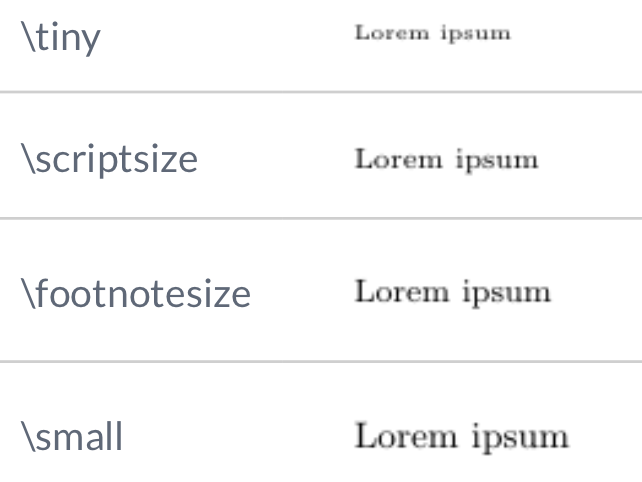
\includegraphics[width=0.5\linewidth]{figures/sample-content/latex_font_sizes} 

}

\caption{Font sizes in LaTeX}\label{fig:latex-font-sizing}
\end{figure}

You could use these to manually adjust the font size in your longtable in two steps:

\begin{enumerate}
\def\labelenumi{\arabic{enumi}.}
\tightlist
\item
  Wrap the longtable environment in, e.g., a \texttt{scriptsize} environment, by doing a string replacement in the output from \texttt{kable}/\texttt{kableExtra}
\item
  Add the attributes that make R Markdown understand that the table is a table (it seems R drops these when we do the string replacement)
\end{enumerate}

\begin{Shaded}
\begin{Highlighting}[]
\NormalTok{our_adjusted_table <-}\StringTok{ }\NormalTok{a_long_table }\OperatorTok\StringTok{ }
\StringTok{  }\KeywordTok{kable}\NormalTok{(}\DataTypeTok{booktabs =} \OtherTok{TRUE}\NormalTok{, }\DataTypeTok{longtable =} \OtherTok{TRUE}\NormalTok{) }\OperatorTok\StringTok{ }
\StringTok{  }\KeywordTok{kable_styling}\NormalTok{(}\DataTypeTok{latex_options =} \StringTok{"repeat_header"}\NormalTok{) }\OperatorTok\StringTok{ }
\StringTok{  }\CommentTok{# wrap the longtable in a tiny environment}
\StringTok{  }\KeywordTok{str_replace}\NormalTok{(}\StringTok{'}\CharTok{\textbackslash{}\textbackslash{}\textbackslash{}\textbackslash{}}\StringTok{begin}\CharTok{\textbackslash{}\textbackslash{}}\StringTok{\{longtable}\CharTok{\textbackslash{}\textbackslash{}}\StringTok{\}'}\NormalTok{, }
              \StringTok{'}\CharTok{\textbackslash{}\textbackslash{}\textbackslash{}\textbackslash{}}\StringTok{begin}\CharTok{\textbackslash{}\textbackslash{}}\StringTok{\{scriptsize}\CharTok{\textbackslash{}\textbackslash{}}\StringTok{\}}\CharTok{\textbackslash{}n\textbackslash{}\textbackslash{}\textbackslash{}\textbackslash{}}\StringTok{begin}\CharTok{\textbackslash{}\textbackslash{}}\StringTok{\{longtable}\CharTok{\textbackslash{}\textbackslash{}}\StringTok{\}'}\NormalTok{) }\OperatorTok
\StringTok{  }\KeywordTok{str_replace}\NormalTok{(}\StringTok{'}\CharTok{\textbackslash{}\textbackslash{}\textbackslash{}\textbackslash{}}\StringTok{end}\CharTok{\textbackslash{}\textbackslash{}}\StringTok{\{longtable}\CharTok{\textbackslash{}\textbackslash{}}\StringTok{\}'}\NormalTok{, }
              \StringTok{'}\CharTok{\textbackslash{}\textbackslash{}\textbackslash{}\textbackslash{}}\StringTok{end}\CharTok{\textbackslash{}\textbackslash{}}\StringTok{\{longtable}\CharTok{\textbackslash{}\textbackslash{}}\StringTok{\}}\CharTok{\textbackslash{}n\textbackslash{}\textbackslash{}\textbackslash{}\textbackslash{}}\StringTok{end}\CharTok{\textbackslash{}\textbackslash{}}\StringTok{\{scriptsize}\CharTok{\textbackslash{}\textbackslash{}}\StringTok{\}'}\NormalTok{)}

\CommentTok{#add attributes to make R Markdown treat this as a kable LaTeX table again}
\NormalTok{our_adjusted_table }\OperatorTok\StringTok{ }
\StringTok{  }\KeywordTok{structure}\NormalTok{(}\DataTypeTok{format =} \StringTok{"latex"}\NormalTok{, }\DataTypeTok{class =} \StringTok{"knitr_kable"}\NormalTok{)}
\end{Highlighting}
\end{Shaded}

\begin{scriptsize}
\begin{longtable}{lrrrrrrrrrrr}
\toprule
  & mpg & cyl & disp & hp & drat & wt & qsec & vs & am & gear & carb\\
\midrule
\endfirsthead
\multicolumn{12}{@{}l}{\textit{(continued)}}\\
\toprule
  & mpg & cyl & disp & hp & drat & wt & qsec & vs & am & gear & carb\\
\midrule
\endhead

\endfoot
\bottomrule
\endlastfoot
Mazda RX4 & 21.0 & 6 & 160.0 & 110 & 3.90 & 2.620 & 16.46 & 0 & 1 & 4 & 4\\
Mazda RX4 Wag & 21.0 & 6 & 160.0 & 110 & 3.90 & 2.875 & 17.02 & 0 & 1 & 4 & 4\\
Datsun 710 & 22.8 & 4 & 108.0 & 93 & 3.85 & 2.320 & 18.61 & 1 & 1 & 4 & 1\\
Hornet 4 Drive & 21.4 & 6 & 258.0 & 110 & 3.08 & 3.215 & 19.44 & 1 & 0 & 3 & 1\\
Hornet Sportabout & 18.7 & 8 & 360.0 & 175 & 3.15 & 3.440 & 17.02 & 0 & 0 & 3 & 2\\
\addlinespace
Valiant & 18.1 & 6 & 225.0 & 105 & 2.76 & 3.460 & 20.22 & 1 & 0 & 3 & 1\\
Duster 360 & 14.3 & 8 & 360.0 & 245 & 3.21 & 3.570 & 15.84 & 0 & 0 & 3 & 4\\
Merc 240D & 24.4 & 4 & 146.7 & 62 & 3.69 & 3.190 & 20.00 & 1 & 0 & 4 & 2\\
Merc 230 & 22.8 & 4 & 140.8 & 95 & 3.92 & 3.150 & 22.90 & 1 & 0 & 4 & 2\\
Merc 280 & 19.2 & 6 & 167.6 & 123 & 3.92 & 3.440 & 18.30 & 1 & 0 & 4 & 4\\
\addlinespace
Merc 280C & 17.8 & 6 & 167.6 & 123 & 3.92 & 3.440 & 18.90 & 1 & 0 & 4 & 4\\
Merc 450SE & 16.4 & 8 & 275.8 & 180 & 3.07 & 4.070 & 17.40 & 0 & 0 & 3 & 3\\
Merc 450SL & 17.3 & 8 & 275.8 & 180 & 3.07 & 3.730 & 17.60 & 0 & 0 & 3 & 3\\
Merc 450SLC & 15.2 & 8 & 275.8 & 180 & 3.07 & 3.780 & 18.00 & 0 & 0 & 3 & 3\\
Cadillac Fleetwood & 10.4 & 8 & 472.0 & 205 & 2.93 & 5.250 & 17.98 & 0 & 0 & 3 & 4\\
\addlinespace
Lincoln Continental & 10.4 & 8 & 460.0 & 215 & 3.00 & 5.424 & 17.82 & 0 & 0 & 3 & 4\\
Chrysler Imperial & 14.7 & 8 & 440.0 & 230 & 3.23 & 5.345 & 17.42 & 0 & 0 & 3 & 4\\
Fiat 128 & 32.4 & 4 & 78.7 & 66 & 4.08 & 2.200 & 19.47 & 1 & 1 & 4 & 1\\
Honda Civic & 30.4 & 4 & 75.7 & 52 & 4.93 & 1.615 & 18.52 & 1 & 1 & 4 & 2\\
Toyota Corolla & 33.9 & 4 & 71.1 & 65 & 4.22 & 1.835 & 19.90 & 1 & 1 & 4 & 1\\
\addlinespace
Toyota Corona & 21.5 & 4 & 120.1 & 97 & 3.70 & 2.465 & 20.01 & 1 & 0 & 3 & 1\\
Dodge Challenger & 15.5 & 8 & 318.0 & 150 & 2.76 & 3.520 & 16.87 & 0 & 0 & 3 & 2\\
AMC Javelin & 15.2 & 8 & 304.0 & 150 & 3.15 & 3.435 & 17.30 & 0 & 0 & 3 & 2\\
Camaro Z28 & 13.3 & 8 & 350.0 & 245 & 3.73 & 3.840 & 15.41 & 0 & 0 & 3 & 4\\
Pontiac Firebird & 19.2 & 8 & 400.0 & 175 & 3.08 & 3.845 & 17.05 & 0 & 0 & 3 & 2\\
\addlinespace
Fiat X1-9 & 27.3 & 4 & 79.0 & 66 & 4.08 & 1.935 & 18.90 & 1 & 1 & 4 & 1\\
Porsche 914-2 & 26.0 & 4 & 120.3 & 91 & 4.43 & 2.140 & 16.70 & 0 & 1 & 5 & 2\\
Lotus Europa & 30.4 & 4 & 95.1 & 113 & 3.77 & 1.513 & 16.90 & 1 & 1 & 5 & 2\\
Ford Pantera L & 15.8 & 8 & 351.0 & 264 & 4.22 & 3.170 & 14.50 & 0 & 1 & 5 & 4\\
Ferrari Dino & 19.7 & 6 & 145.0 & 175 & 3.62 & 2.770 & 15.50 & 0 & 1 & 5 & 6\\
\addlinespace
Maserati Bora & 15.0 & 8 & 301.0 & 335 & 3.54 & 3.570 & 14.60 & 0 & 1 & 5 & 8\\
Volvo 142E & 21.4 & 4 & 121.0 & 109 & 4.11 & 2.780 & 18.60 & 1 & 1 & 4 & 2\\
Mazda RX41 & 21.0 & 6 & 160.0 & 110 & 3.90 & 2.620 & 16.46 & 0 & 1 & 4 & 4\\
Mazda RX4 Wag1 & 21.0 & 6 & 160.0 & 110 & 3.90 & 2.875 & 17.02 & 0 & 1 & 4 & 4\\
Datsun 7101 & 22.8 & 4 & 108.0 & 93 & 3.85 & 2.320 & 18.61 & 1 & 1 & 4 & 1\\
\addlinespace
Hornet 4 Drive1 & 21.4 & 6 & 258.0 & 110 & 3.08 & 3.215 & 19.44 & 1 & 0 & 3 & 1\\
Hornet Sportabout1 & 18.7 & 8 & 360.0 & 175 & 3.15 & 3.440 & 17.02 & 0 & 0 & 3 & 2\\
Valiant1 & 18.1 & 6 & 225.0 & 105 & 2.76 & 3.460 & 20.22 & 1 & 0 & 3 & 1\\
Duster 3601 & 14.3 & 8 & 360.0 & 245 & 3.21 & 3.570 & 15.84 & 0 & 0 & 3 & 4\\
Merc 240D1 & 24.4 & 4 & 146.7 & 62 & 3.69 & 3.190 & 20.00 & 1 & 0 & 4 & 2\\
\addlinespace
Merc 2301 & 22.8 & 4 & 140.8 & 95 & 3.92 & 3.150 & 22.90 & 1 & 0 & 4 & 2\\
Merc 2801 & 19.2 & 6 & 167.6 & 123 & 3.92 & 3.440 & 18.30 & 1 & 0 & 4 & 4\\
Merc 280C1 & 17.8 & 6 & 167.6 & 123 & 3.92 & 3.440 & 18.90 & 1 & 0 & 4 & 4\\
Merc 450SE1 & 16.4 & 8 & 275.8 & 180 & 3.07 & 4.070 & 17.40 & 0 & 0 & 3 & 3\\
Merc 450SL1 & 17.3 & 8 & 275.8 & 180 & 3.07 & 3.730 & 17.60 & 0 & 0 & 3 & 3\\
\addlinespace
Merc 450SLC1 & 15.2 & 8 & 275.8 & 180 & 3.07 & 3.780 & 18.00 & 0 & 0 & 3 & 3\\
Cadillac Fleetwood1 & 10.4 & 8 & 472.0 & 205 & 2.93 & 5.250 & 17.98 & 0 & 0 & 3 & 4\\
Lincoln Continental1 & 10.4 & 8 & 460.0 & 215 & 3.00 & 5.424 & 17.82 & 0 & 0 & 3 & 4\\
Chrysler Imperial1 & 14.7 & 8 & 440.0 & 230 & 3.23 & 5.345 & 17.42 & 0 & 0 & 3 & 4\\
Fiat 1281 & 32.4 & 4 & 78.7 & 66 & 4.08 & 2.200 & 19.47 & 1 & 1 & 4 & 1\\
\addlinespace
Honda Civic1 & 30.4 & 4 & 75.7 & 52 & 4.93 & 1.615 & 18.52 & 1 & 1 & 4 & 2\\
Toyota Corolla1 & 33.9 & 4 & 71.1 & 65 & 4.22 & 1.835 & 19.90 & 1 & 1 & 4 & 1\\
Toyota Corona1 & 21.5 & 4 & 120.1 & 97 & 3.70 & 2.465 & 20.01 & 1 & 0 & 3 & 1\\
Dodge Challenger1 & 15.5 & 8 & 318.0 & 150 & 2.76 & 3.520 & 16.87 & 0 & 0 & 3 & 2\\
AMC Javelin1 & 15.2 & 8 & 304.0 & 150 & 3.15 & 3.435 & 17.30 & 0 & 0 & 3 & 2\\
\addlinespace
Camaro Z281 & 13.3 & 8 & 350.0 & 245 & 3.73 & 3.840 & 15.41 & 0 & 0 & 3 & 4\\
Pontiac Firebird1 & 19.2 & 8 & 400.0 & 175 & 3.08 & 3.845 & 17.05 & 0 & 0 & 3 & 2\\
Fiat X1-91 & 27.3 & 4 & 79.0 & 66 & 4.08 & 1.935 & 18.90 & 1 & 1 & 4 & 1\\
Porsche 914-21 & 26.0 & 4 & 120.3 & 91 & 4.43 & 2.140 & 16.70 & 0 & 1 & 5 & 2\\
Lotus Europa1 & 30.4 & 4 & 95.1 & 113 & 3.77 & 1.513 & 16.90 & 1 & 1 & 5 & 2\\
\addlinespace
Ford Pantera L1 & 15.8 & 8 & 351.0 & 264 & 4.22 & 3.170 & 14.50 & 0 & 1 & 5 & 4\\
Ferrari Dino1 & 19.7 & 6 & 145.0 & 175 & 3.62 & 2.770 & 15.50 & 0 & 1 & 5 & 6\\
Maserati Bora1 & 15.0 & 8 & 301.0 & 335 & 3.54 & 3.570 & 14.60 & 0 & 1 & 5 & 8\\
Volvo 142E1 & 21.4 & 4 & 121.0 & 109 & 4.11 & 2.780 & 18.60 & 1 & 1 & 4 & 2\\*
\end{longtable}
\end{scriptsize}

\begin{savequote}
There is grandeur in this view of life, with its several powers, having
been originally breathed into a few forms or into one; and that, whilst
this planet has gone cycling on according to the fixed law of gravity,
from so simple a beginning endless forms most beautiful and most
wonderful have been, and are being, evolved.
\qauthor{--- Charles Darwin \autocite{Darwin1859}}\end{savequote}



\hypertarget{customisations-and-extensions}{%
\chapter{Customisations and extensions}\label{customisations-and-extensions}}

\minitoc 

\noindent This chapter describes a number of additional tips and tricks as well as possible customizations to the \texttt{oxforddown} thesis.

\hypertarget{front-matter}{%
\section{Front matter}\label{front-matter}}

\hypertarget{shorten-captions-shown-in-the-list-of-figures-pdf}{%
\subsection{Shorten captions shown in the list of figures (PDF)}\label{shorten-captions-shown-in-the-list-of-figures-pdf}}

You might want your list of figures (which follows the table of contents) to have shorter (or just different) figure descriptions than the actual figure captions.

Do this using the chunk option \texttt{fig.scap} (`short caption'), for example \texttt{\{r\ captain-image,\ fig.cap="A\ very\ long\ and\ descriptive\ (and\ potentially\ boring)\ caption\ that\ doesn\textquotesingle{}t\ fit\ in\ the\ list\ of\ figures,\ but\ helps\ the\ reader\ understand\ what\ the\ figure\ communicates.",\ fig.scap="A\ concise\ description\ for\ the\ list\ of\ figures"}

\hypertarget{shorten-captions-shown-in-the-list-of-tables-pdf}{%
\subsection{Shorten captions shown in the list of tables (PDF)}\label{shorten-captions-shown-in-the-list-of-tables-pdf}}

You might want your list of tables (which follows the list of figures in your thesis front matter) to have shorter (or just different) table descriptions than the actual table captions.

If you are using \texttt{knitr::kable} to generate a table, you can do this with the argument \texttt{caption.short}, e.g.:

\begin{Shaded}
\begin{Highlighting}[]
\NormalTok{knitr}\OperatorTok{::}\KeywordTok{kable}\NormalTok{(mtcars,}
              \DataTypeTok{caption =} \StringTok{"A very long and descriptive (and potentially}
\StringTok{              boring) caption that doesn't fit in the list of figures,}
\StringTok{              but helps the reader understand what the figure }
\StringTok{              communicates."}\NormalTok{,}
              \DataTypeTok{caption.short =} \StringTok{"A concise description for the list of tables"}\NormalTok{)}
\end{Highlighting}
\end{Shaded}

\hypertarget{shorten-running-header-pdf}{%
\section{Shorten running header (PDF)}\label{shorten-running-header-pdf}}

You might want a chapter's running header (i.e.~the header showing the title of the current chapter at the top of page) to be shorter (or just different) to the actual chapter title.

Do this by adding the latex command \texttt{\textbackslash{}chaptermark\{My\ shorter\ version\}} after your chapter title.

For example, chapter \ref{cites-and-refs}`s running header is simply 'Cites and cross-refs', because it begins like this:

\begin{Shaded}
\begin{Highlighting}[]
\FunctionTok{# Citations, cross-references, and collaboration \{#cites-and-refs\} }
\NormalTok{\textbackslash{}chaptermark\{Cites and cross-refs\}}
\end{Highlighting}
\end{Shaded}

\hypertarget{unnumbered-chapters}{%
\section{Unnumbered chapters}\label{unnumbered-chapters}}

To make chapters unnumbered (normally only relevant to the Introduction and/or the Conclusion), follow the chapter header with \texttt{\{-\}}, e.g.~\texttt{\#\ Introduction\ \{-\}}.

When you do this, you must also follow the heading with these two latex commands:

\begin{Shaded}
\begin{Highlighting}[]
\FunctionTok{\textbackslash{}adjustmtc}
\FunctionTok{\textbackslash{}markboth}\NormalTok{\{The Name of Your Unnumbered Chapter\}\{\}}
\end{Highlighting}
\end{Shaded}

Otherwise the chapter's mini table of contents and the running header will show the previous chapter.

\hypertarget{beginning-chapters-with-quotes-pdf}{%
\section{Beginning chapters with quotes (PDF)}\label{beginning-chapters-with-quotes-pdf}}

The OxThesis LaTeX template lets you inject some wittiness into your thesis by including a block of type \texttt{savequote} at the beginning of chapters.
To do this, use the syntax \texttt{\textasciigrave{}\textasciigrave{}\textasciigrave{}\{block\ type=\textquotesingle{}savequote\textquotesingle{}\}}.\footnote{For more on custom block types, see the relevant section in \href{https://bookdown.org/yihui/bookdown/custom-blocks.html}{\emph{Authoring Books with R Markdown}}.}

Add the reference for the quote with the chunk option \texttt{quote\_author="my\ author\ name"}.
You will also want to add the chunk option \texttt{include=knitr::is\_latex\_output()} so that quotes are only included in PDF output.

It's not possible to use markdown syntax inside chunk options, so if you want to e.g.~italicise a book name in the reference use a \href{https://bookdown.org/yihui/bookdown/markdown-extensions-by-bookdown.html\#text-references}{`text reference'}: Create a named piece of text with `(ref:label-name) My text', then point to this in the chunk option with \texttt{quote\_author=\textquotesingle{}(ref:label-name)\textquotesingle{}}.

\hypertarget{highlighting-corrections-html-pdf}{%
\section{Highlighting corrections (HTML \& PDF)}\label{highlighting-corrections-html-pdf}}

For when it comes time to do corrections, you may want to highlight changes made when you submit a post-viva, corrected copy to your examiners so they can quickly verify you've completed the task.
You can do so like this:

\hypertarget{short-inline-corrections}{%
\subsection{Short, inline corrections}\label{short-inline-corrections}}

Highlight \textbf{short, inline corrections} by doing \texttt{{[}like\ this{]}\{.correction\}} --- the text between the square brackets will then \hl{be highlighted in blue} in the output.

Note that pandoc might get confused by citations and cross-references inside inline corrections.
In particular, it might get confused by \texttt{"{[}what\ @Shea2014\ said{]}\{.correction\}"} which becomes \autocite[what][ said]{Shea2014}\{.correction\}
In such cases, you can use LaTeX syntax directly.
The correction highlighting uses the \href{https://ctan.org/pkg/soul}{soul} package, so you can do like this:

\begin{itemize}
\tightlist
\item
  If using biblatex for references, use \texttt{"\textbackslash{}hl\{what\ \textbackslash{}textcite\{Shea2014\}\ said\}}
\item
  If using natbib for references, use \texttt{"\textbackslash{}hl\{what\ \textbackslash{}cite\{Shea2014\}\ said\}}
\end{itemize}

Using raw LaTeX has the drawback of corrections then not showing up in HTML output at all, but you might only care about correction highlighting in the PDF for your examiners anyway!

\hypertarget{blocks-of-added-or-changed-material}{%
\subsection{Blocks of added or changed material}\label{blocks-of-added-or-changed-material}}

Highlight entire \textbf{blocks of added or changed material} by putting them in a block of type \texttt{correction}, using the syntax \texttt{\textasciigrave{}\textasciigrave{}\textasciigrave{}\{block\ type=\textquotesingle{}correction\textquotesingle{}\}}.\footnote{In the \textbf{.tex} file for PDF output, this will put the content between \texttt{\textbackslash{}begin\{correction\}} and \texttt{\textbackslash{}end\{correction\}}; in gitbook output it will be put between \texttt{\textless{}div\ class="correction"\textgreater{}} and \texttt{\textless{}/div\textgreater{}}.}
Like so:

\begin{correction}
For larger chunks, like this paragraph or indeed entire figures, you can
use the \texttt{correction} block type. This environment
\textbf{highlights paragraph-sized and larger blocks} with the same blue
colour.
\end{correction}

\emph{Note that correction blocks cannot be included in word output.}

\hypertarget{stopping-corrections-from-being-highlighted}{%
\subsection{Stopping corrections from being highlighted}\label{stopping-corrections-from-being-highlighted}}

To turn off correction highlighting, go to the YAML header of \textbf{index.Rmd}, then:

\begin{itemize}
\tightlist
\item
  PDF output: set \texttt{corrections:\ false}\\
\item
  HTML output: remove or comment out \texttt{-\ templates/corrections.css}
\end{itemize}

\hypertarget{apply-custom-font-color-and-highlighting-to-text-html-pdf}{%
\section{Apply custom font color and highlighting to text (HTML \& PDF)}\label{apply-custom-font-color-and-highlighting-to-text-html-pdf}}

The lua filter that adds the functionality to highlight corrections adds two more tricks:
you can apply your own choice of colour to highlight text, or change the font color.
The syntax is as follows:

\begin{quote}
Here's \texttt{{[}some\ text\ in\ pink\ highlighting{]}\{highlight="pink"\}}\\
Becomes: Here's \sethlcolor{pink}\hl{some text in pink highlighting}\sethlcolor{correctioncolor}.
\end{quote}

\begin{quote}
\texttt{{[}Here\textquotesingle{}s\ some\ text\ with\ blue\ font{]}\{color="blue"\}}~\\
Becomes: \textcolor{blue}{Here's some text with blue font}
\end{quote}

\begin{quote}
Finally --- never, ever actually do this -- \texttt{{[}here\textquotesingle{}s\ some\ text\ with\ black\ highlighting\ and\ yellow\ font{]}\{highlight="black"\ color="yellow"\}}\\
Becomes: \textcolor{yellow}{\sethlcolor{black}\hl{here's some text with black highlighting and yellow font}\sethlcolor{correctioncolor}}
\end{quote}

The file \textbf{scripts\_and\_filters/colour\_and\_highlight.lua} implements this, if you want to fiddle around with it.
It works with both PDF and HTML output.

\hypertarget{embed-pdf}{%
\section{Including another paper in your thesis - embed a PDF document}\label{embed-pdf}}

You may want to embed existing PDF documents into the thesis, for example if your department allows a `portfolio' style thesis and you need to include an existing typeset publication as a chapter.

In gitbook output, you can simply use \texttt{knitr::include\_graphics} and it should include a scrollable (and downloadable) PDF.
You will probably want to set the chunk options \texttt{out.width=\textquotesingle{}100\%\textquotesingle{}} and \texttt{out.height=\textquotesingle{}1000px\textquotesingle{}}:

\begin{Shaded}
\begin{Highlighting}[]
\NormalTok{knitr}\OperatorTok{::}\KeywordTok{include_graphics}\NormalTok{(}\StringTok{"figures/sample-content/pdf_embed_example/Lyngs2020_FB.pdf"}\NormalTok{)}
\end{Highlighting}
\end{Shaded}

In LaTeX output, however, this approach can cause odd behaviour.
Therefore, when you build your thesis to PDF, split the PDF into an alphanumerically sorted sequence of \textbf{single-page} PDF files (you can do this automatically with the package \texttt{pdftools}). You can then use the appropriate LaTeX command to insert them, as shown below (for brevity, in the \texttt{oxforddown} PDF sample content we're only including two pages).
\emph{Note that the chunk option \texttt{results=\textquotesingle{}asis\textquotesingle{}} must be set.}
You may also want to remove margins from the PDF files, which you can do with Adobe Acrobat (paid version) and likely other software.

\begin{Shaded}
\begin{Highlighting}[]
\CommentTok{# install.packages(pdftools)}
\CommentTok{# split PDF into pages stored in}
\NormalTok{    figures}\OperatorTok{/}\NormalTok{sample}\OperatorTok{-}\NormalTok{content}\OperatorTok{/}\NormalTok{pdf_embed_example}\OperatorTok{/}\NormalTok{split}\OperatorTok{/}
\CommentTok{#}
\StringTok{    }\NormalTok{pdftools}\OperatorTok{::}\KeywordTok{pdf_split}\NormalTok{(}\StringTok{"figures/sample-content/pdf_embed_example/Lyngs2020_FB.pdf"}\NormalTok{,}
\CommentTok{# output = "figures/sample-content/pdf_embed_example/split/")}

\CommentTok{# grab the pages}
\NormalTok{pages <-}\StringTok{ }\KeywordTok{list.files}\NormalTok{(}\StringTok{"figures/sample-content/pdf_embed_example/split"}\NormalTok{,}
    \DataTypeTok{full.names =} \OtherTok{TRUE}\NormalTok{)}

\CommentTok{# set how wide you want the inserted PDFs to be:}
\CommentTok{# 1.0 is 100 per cent of the oxforddown PDF page width;}
\CommentTok{# you may want to make it a bit bigger}
\NormalTok{pdf_width <-}\StringTok{ }\FloatTok{1.2}

\CommentTok{# for each PDF page, insert it nicely and}
\CommentTok{# end with a page break}
\KeywordTok{cat}\NormalTok{(stringr}\OperatorTok{::}\KeywordTok{str_c}\NormalTok{(}\StringTok{"}\CharTok{\textbackslash{}\textbackslash{}}\StringTok{newpage }\CharTok{\textbackslash{}\textbackslash{}}\StringTok{begin\{center\}}
\StringTok{    }\CharTok{\textbackslash{}\textbackslash{}}\StringTok{makebox[}\CharTok{\textbackslash{}\textbackslash{}}\StringTok{linewidth][c]\{}\CharTok{\textbackslash{}\textbackslash{}}\StringTok{includegraphics[width="}\NormalTok{, pdf_width,}
    \StringTok{"}\CharTok{\textbackslash{}\textbackslash{}}\StringTok{linewidth]\{"}\NormalTok{, pages, }\StringTok{"\}\} }\CharTok{\textbackslash{}\textbackslash{}}\StringTok{end\{center\}"}\NormalTok{))}
\end{Highlighting}
\end{Shaded}

\newpage \begin{center} \makebox[\linewidth][c]{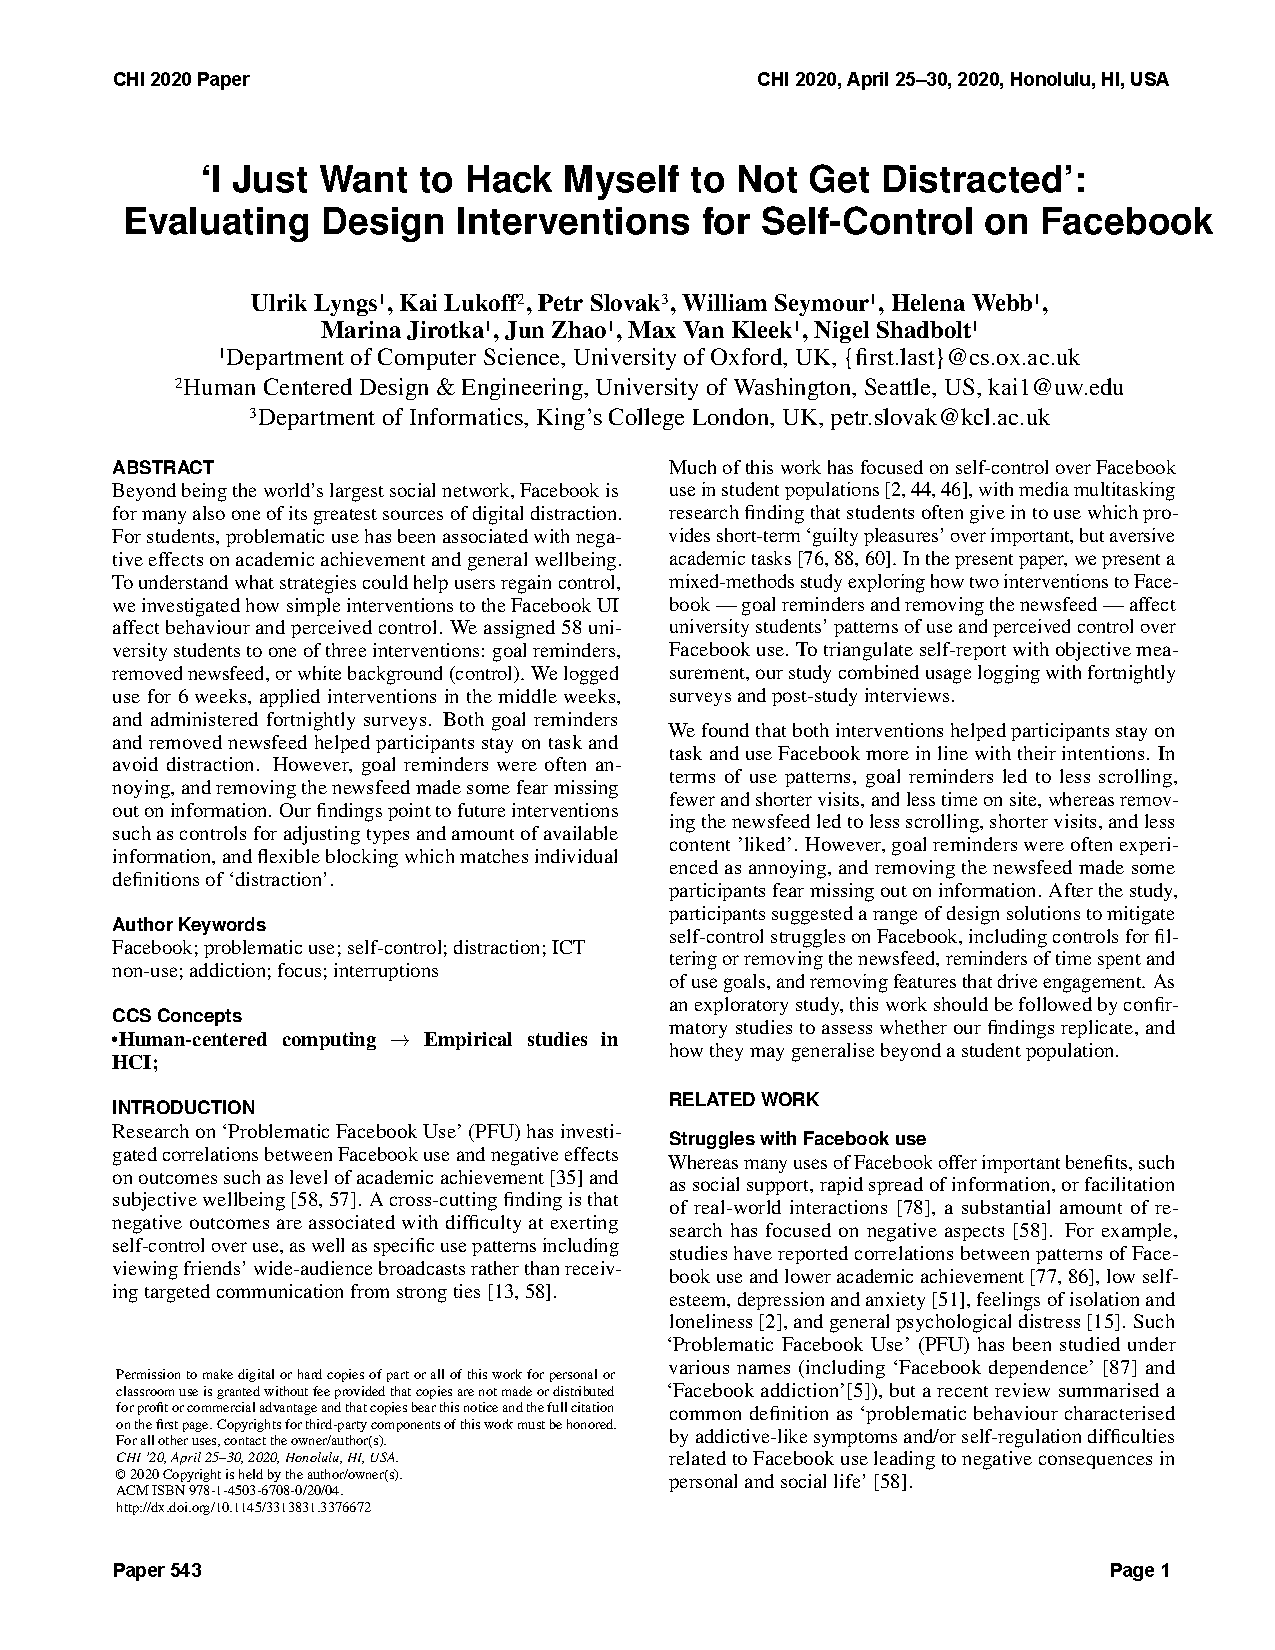
\includegraphics[width=1.2\linewidth]{figures/sample-content/pdf_embed_example/split/_000000000000001.pdf}} \end{center} \newpage \begin{center} \makebox[\linewidth][c]{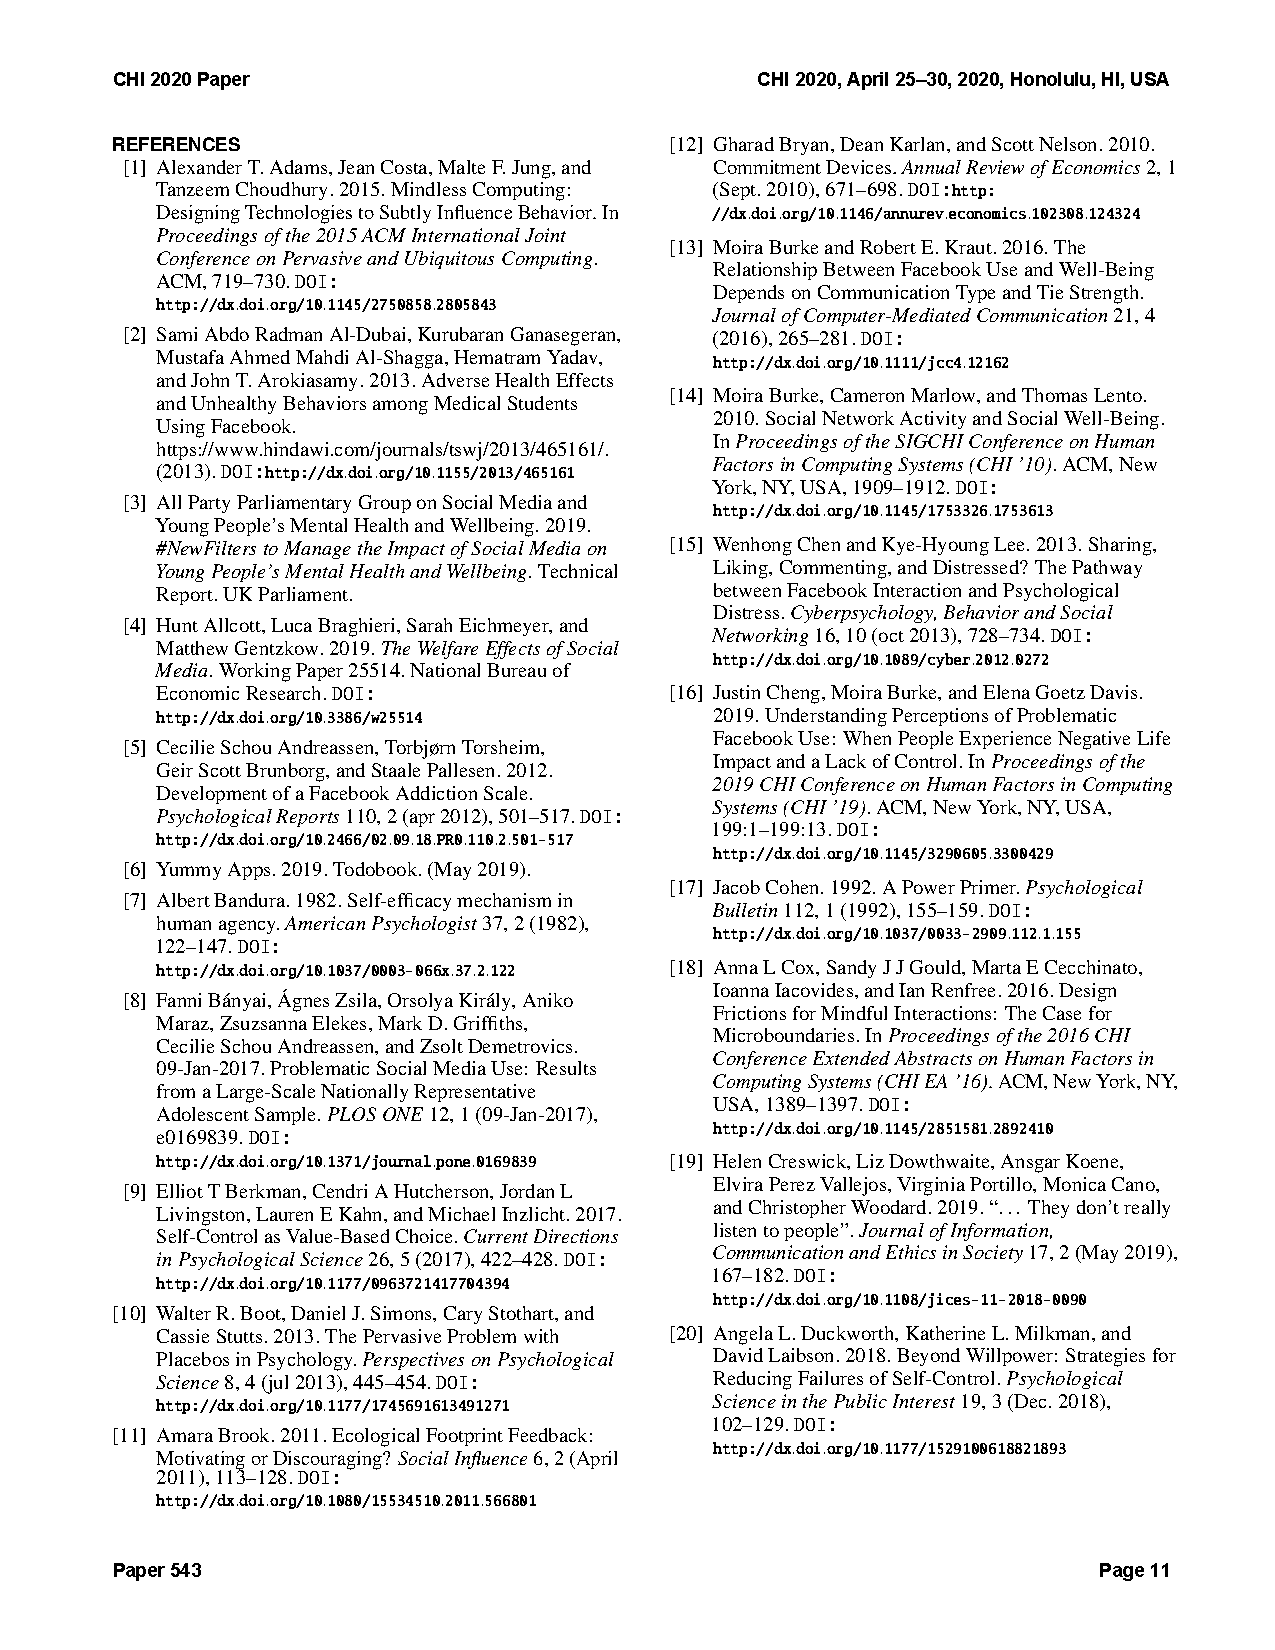
\includegraphics[width=1.2\linewidth]{figures/sample-content/pdf_embed_example/split/_000000000000011.pdf}} \end{center}

\hypertarget{embed-rmd}{%
\section{Including another paper in your thesis - R Markdown child document}\label{embed-rmd}}

Sometimes you want to include another paper you are currently writing as a chapter in your thesis.
Above \ref{embed-pdf}, we described the simplest way to do this: include the other paper as a pdf.
However, in some cases you instead want to include the R Markdown source from this paper, and have it compiled within your thesis.
This is a little bit more tricky, because you need to keep careful track of your file paths, but it is possible by \href{https://bookdown.org/yihui/rmarkdown-cookbook/child-document.html}{including the paper as a child document}.
There are four main steps:

\begin{enumerate}
\def\labelenumi{\arabic{enumi}.}
\tightlist
\item
  Include the paper as a child document
\item
  Make file paths compatible with knitting the article on its own, as well as when it's include in your thesis
\item
  Make header levels correct
\item
  Make figure widths correct
\end{enumerate}

\hypertarget{an-example-paper-in-another-folder}{%
\subsection{An example paper in another folder}\label{an-example-paper-in-another-folder}}

Take this simple example (files for this are in \href{https://github.com/ulyngs/oxforddown-external-article}{this GitHub repository}):

\begin{Shaded}
\begin{Highlighting}[]
\NormalTok{|--paper_to_include}
\NormalTok{|  |--my_paper.Rmd}
\NormalTok{|  |--data}
\NormalTok{|  |  |--cat_salt.csv}
\NormalTok{|  |--figures}
\NormalTok{|  |  |--cat.jpg}
\NormalTok{|}
\NormalTok{|--thesis}
\end{Highlighting}
\end{Shaded}

As the chart suggests, you have another folder, \textbf{paper\_to\_include/} living in the same containing folder as your thesis folder.
In the \textbf{paper\_to\_include} folder, the file \textbf{my\_paper.Rmd} is where you write the paper.
In \textbf{my\_paper.Rmd}, you read in a CSV file found in the subfolder \textbf{data/cats.csv}, and also an image from the subfolder \textbf{figures/cat.jpg}.

\hypertarget{step-1-include-paper-as-a-child-document}{%
\subsection{Step 1: Include paper as a child document}\label{step-1-include-paper-as-a-child-document}}

In your thesis folder, create an Rmd file for the chapter where you want to include another paper.
Add one or more code chunks that include R Markdown files from that paper as child documents:

\begin{Shaded}
\begin{Highlighting}[]
\FunctionTok{# Including an external chapter }

\BaseNTok{```\{r child = "../paper_to_include/my_paper.Rmd"\}}
\BaseNTok{```}
\end{Highlighting}
\end{Shaded}

\hypertarget{step-2-make-file-paths-compatible}{%
\subsection{Step 2: Make file paths compatible}\label{step-2-make-file-paths-compatible}}

Use \href{https://rmarkdown.rstudio.com/lesson-6.html}{parameters} to adjust the file path of images based on values you set in the YAML header of an R Markdown file.
In \textbf{my\_paper.Rmd}, create a parameter called \texttt{other\_path} and set it to an empty string:

\begin{Shaded}
\begin{Highlighting}[]
\PreprocessorTok{---}
\FunctionTok{title}\KeywordTok{:}\AttributeTok{ }\StringTok{"A fabulous article in a different folder"}
\FunctionTok{params}\KeywordTok{:}
\AttributeTok{  }\FunctionTok{other_path}\KeywordTok{:}\AttributeTok{ }\StringTok{""}
\PreprocessorTok{---}
\end{Highlighting}
\end{Shaded}

In \textbf{my\_paper.Rmd}, put this at the start of the filepath when you read in data or include images:

\begin{Shaded}
\begin{Highlighting}[]
\KeywordTok{library}\NormalTok{(tidyverse)}
\KeywordTok{library}\NormalTok{(knitr)}

\NormalTok{cat_data <-}\StringTok{ }\KeywordTok{read_csv}\NormalTok{(}\KeywordTok{str_c}\NormalTok{(params}\OperatorTok{$}\NormalTok{other_path, }\StringTok{"data/cats.csv"}\NormalTok{))}
\KeywordTok{include_graphics}\NormalTok{(}\KeywordTok{str_c}\NormalTok{(params}\OperatorTok{$}\NormalTok{other_path, }\StringTok{"figures/cat.jpg"}\NormalTok{))}
\end{Highlighting}
\end{Shaded}

Finally, in your thesis folder's \textbf{index.Rmd} file, also create the parameter \texttt{other\_path}.
But here, set it to where the \textbf{paper\_to\_include/} folder is relative to your thesis folder:

\begin{Shaded}
\begin{Highlighting}[]
\FunctionTok{params}\KeywordTok{:}
\AttributeTok{  }\FunctionTok{other_path}\KeywordTok{:}\AttributeTok{ }\StringTok{"../paper_to_include/"}
\end{Highlighting}
\end{Shaded}

\hypertarget{note-on-html-output}{%
\subsubsection{Note on HTML output}\label{note-on-html-output}}

Note that if you want to host an HTML version on your thesis online, you will need to include graphics in the content that you host online - the internet obviously won't be able to see filepaths that are just referring to stuff in another folder on your computer!

\hypertarget{step-3-make-sure-header-levels-are-correct}{%
\subsection{Step 3: Make sure header levels are correct}\label{step-3-make-sure-header-levels-are-correct}}

Unless the paper you want to include is also written as a book, your header levels are probably going to be off.
That is, the level 1 headers (\# Some header) you use for main sections in the other paper turns into chaper titles when included in your thesis.

To avoid this, first \emph{increment all heading levels by one in \textbf{paper\_to\_include/my\_paper.Rmd}} (\# Some header -\textgreater{} \#\# Some header).
Then in \textbf{paper\_to\_include/} create a \href{https://bookdown.org/yihui/rmarkdown-cookbook/lua-filters.html\#lua-filters}{lua filter} that decrements header levels by one: Create a text file, save it as \textbf{reduce\_header\_level.lua}, and give it the content below.

\begin{Shaded}
\begin{Highlighting}[]
\KeywordTok{function}\NormalTok{ Header}\OperatorTok{(}\NormalTok{el}\OperatorTok{)}
  \ControlFlowTok{if} \OperatorTok{(}\NormalTok{el}\OperatorTok{.}\NormalTok{level }\OperatorTok{<=} \DecValTok{1}\OperatorTok{)} \ControlFlowTok{then}
    \FunctionTok{error}\OperatorTok{(}\StringTok{"I don't know how to decrease the level of h1"}\OperatorTok{)}
  \ControlFlowTok{end}
\NormalTok{  el}\OperatorTok{.}\NormalTok{level }\OperatorTok{=}\NormalTok{ el}\OperatorTok{.}\NormalTok{level }\OperatorTok{-} \DecValTok{1}
  \ControlFlowTok{return}\NormalTok{ el}
\ControlFlowTok{end}
\end{Highlighting}
\end{Shaded}

In the YAML header of \textbf{paper\_to\_include/my\_paper.Rmd}, use this filter:

\begin{Shaded}
\begin{Highlighting}[]
\PreprocessorTok{---}
\FunctionTok{title}\KeywordTok{:}\AttributeTok{ }\StringTok{"A fabulous article in a different folder"}
\FunctionTok{params}\KeywordTok{:}
\AttributeTok{  }\FunctionTok{other_path}\KeywordTok{:}\AttributeTok{ }\StringTok{""}
\FunctionTok{output}\KeywordTok{:}
\AttributeTok{  }\FunctionTok{pdf_document}\KeywordTok{:}\AttributeTok{ }
\AttributeTok{    }\FunctionTok{pandoc_args}\KeywordTok{:}\AttributeTok{ }\KeywordTok{[}\StringTok{"--lua-filter=reduce_header_level.lua"}\KeywordTok{]}
\PreprocessorTok{---}
\end{Highlighting}
\end{Shaded}

Now, your header levels will be correct both when you knit the paper on its own and when its included in your thesis.

NOTE: There might be no need to use a lua filter to shift heading - it seems you could simply use \texttt{pandoc\_args:\ {[}"-\/-shift-heading-level-by=-1"{]}} (see \url{https://pandoc.org/MANUAL.html\#reader-options})

\hypertarget{step-4.-make-sure-figure-widths-are-correct}{%
\subsection{Step 4. Make sure figure widths are correct}\label{step-4.-make-sure-figure-widths-are-correct}}

It might be that your figure widths when knitting your paper on its own, and when including it in your thesis, need to be different.
You can again use parameters to set figure widths.

Imagine you want figure width to be 80\% of the page width when knitting your paper on its own, but 100\% in your thesis.
In \textbf{paper\_to\_include/my\_paper.Rmd}, first add a parameter we could call \texttt{out\_width} and set it to the string ``80\%'':

\begin{Shaded}
\begin{Highlighting}[]
\PreprocessorTok{---}
\FunctionTok{title}\KeywordTok{:}\AttributeTok{ }\StringTok{"A fabulous article in a different folder"}
\FunctionTok{params}\KeywordTok{:}
\AttributeTok{  }\FunctionTok{other_path}\KeywordTok{:}\AttributeTok{ }\StringTok{""}
\AttributeTok{  }\FunctionTok{out_width}\KeywordTok{:}\AttributeTok{ }\StringTok{"80%"}
\FunctionTok{output}\KeywordTok{:}
\AttributeTok{  }\FunctionTok{pdf_document}\KeywordTok{:}\AttributeTok{ }
\AttributeTok{    }\FunctionTok{pandoc_args}\KeywordTok{:}\AttributeTok{ }\KeywordTok{[}\StringTok{"--lua-filter=reduce_header_level.lua"}\KeywordTok{]}
\PreprocessorTok{---}
\end{Highlighting}
\end{Shaded}

Then, make sure use that parameter to set the output width when you include figures in \textbf{paper\_to\_include/my\_paper.Rmd}:

\begin{Shaded}
\begin{Highlighting}[]
\BaseNTok{```\{r, out.width=params$out_width, fig.cap="A very funny cat"\}}
\BaseNTok{include_graphics(str_c(params$other_path, "figures/cat.jpg"))}
\BaseNTok{```}
\end{Highlighting}
\end{Shaded}

Finally, create the parameter \texttt{out\_width} in your thesis' \textbf{index.Rmd} file:

\begin{Shaded}
\begin{Highlighting}[]
\FunctionTok{params}\KeywordTok{:}
\AttributeTok{  }\FunctionTok{other_path}\KeywordTok{:}\AttributeTok{ }\StringTok{"../paper_to_include/"}
\AttributeTok{  }\FunctionTok{out_width}\KeywordTok{:}\AttributeTok{ }\StringTok{"80%"}
\end{Highlighting}
\end{Shaded}

Now, the output width of your figure will be 80\% when knitting your paper on its own, and 100\% when knitting it as child document of your thesis.

\hypertarget{customizing-referencing}{%
\section{Customizing referencing}\label{customizing-referencing}}

\hypertarget{using-a-.csl-file-with-pandoc-instead-of-biblatex}{%
\subsection{Using a .csl file with pandoc instead of biblatex}\label{using-a-.csl-file-with-pandoc-instead-of-biblatex}}

The \texttt{oxforddown} package uses biblatex in LaTeX for referencing.
It is also possible to use pandoc for referencing by providing a .csl file in the YAML header of \textbf{index.Rmd} (likely requiring commenting out the biblatex code in \textbf{templates/template.tex}).
This may be helpful for those who have a .csl file describing the referencing format for a particular journal.
However, note that this approach does not support chapter bibliographies (see Section \ref{biblatex-custom}).

\begin{Shaded}
\begin{Highlighting}[]
\FunctionTok{csl}\KeywordTok{:}\AttributeTok{ ecology.csl}
\end{Highlighting}
\end{Shaded}

\hypertarget{biblatex-custom}{%
\subsection{Customizing biblatex and adding chapter bibliographies}\label{biblatex-custom}}

This section provides one example of customizing biblatex. Much of this code was combined from searches on Stack Exchange and other sources (e.g.~\href{https://tex.stackexchange.com/questions/10682/suppress-in-biblatex}{here}).

In \textbf{templates/template.tex}, one can replace the existing biblatex calls with the following to achieve referencing that looks like this:

(Charmantier and Gienapp 2014)

Charmantier, A. and P. Gienapp (2014). Climate change and timing of avian breeding and migration: evolutionary versus plastic changes. Evolutionary Applications 7(1):15--28. doi: 10.1111/eva.12126.

\begin{Shaded}
\begin{Highlighting}[]
\BuiltInTok{\textbackslash{}usepackage}\NormalTok{[backend=biber,}
\NormalTok{    bibencoding=utf8,}
\NormalTok{    refsection=chapter, }\CommentTok{% referencing by chapter}
\NormalTok{    style=authoryear, }
\NormalTok{    firstinits=true,}
\NormalTok{    isbn=false,}
\NormalTok{    doi=true,}
\NormalTok{    url=false,}
\NormalTok{    eprint=false,}
\NormalTok{    related=false,}
\NormalTok{    dashed=false,}
\NormalTok{    clearlang=true,}
\NormalTok{    maxcitenames=2,}
\NormalTok{    mincitenames=1,}
\NormalTok{    maxbibnames=10,}
\NormalTok{    abbreviate=false,}
\NormalTok{    minbibnames=3,}
\NormalTok{    uniquelist=minyear,}
\NormalTok{    sortcites=true,}
\NormalTok{    date=year}
\NormalTok{]\{}\ExtensionTok{biblatex}\NormalTok{\}}
\FunctionTok{\textbackslash{}AtEveryBibitem}\NormalTok{\{}\CommentTok
  \FunctionTok{\textbackslash{}clearfield}\NormalTok{\{note\}}
\NormalTok{\}}

\FunctionTok{\textbackslash{}DeclareFieldFormat}\NormalTok{\{titlecase\}\{}\FunctionTok{\textbackslash{}MakeTitleCase}\NormalTok{\{#1\}\}}

\FunctionTok{\textbackslash{}newrobustcmd}\NormalTok{\{}\FunctionTok{\textbackslash{}MakeTitleCase}\NormalTok{\}[1]\{}\CommentTok
    \FunctionTok{\textbackslash{}OR\textbackslash{}ifcurrentfield}\NormalTok{\{maintitle\}}\FunctionTok{\textbackslash{}OR\textbackslash{}ifcurrentfield}\NormalTok{\{mainsubtitle\}}\CommentTok
    \FunctionTok{\textbackslash{}OR\textbackslash{}ifcurrentfield}\NormalTok{\{issuetitle\}}\FunctionTok{\textbackslash{}OR\textbackslash{}ifcurrentfield}\NormalTok{\{issuesubtitle\}}\CommentTok
    \FunctionTok{\textbackslash{}OR\textbackslash{}ifentrytype}\NormalTok{\{booklet\}}\FunctionTok{\textbackslash{}OR\textbackslash{}ifentrytype}\NormalTok{\{suppbook\}}\CommentTok
    \FunctionTok{\textbackslash{}OR\textbackslash{}ifentrytype}\NormalTok{\{suppcollection\}}\FunctionTok{\textbackslash{}OR\textbackslash{}ifentrytype}\NormalTok{\{manual\}}\CommentTok
    \FunctionTok{\textbackslash{}OR\textbackslash{}ifentrytype}\NormalTok{\{proceedings\}}\FunctionTok{\textbackslash{}OR\textbackslash{}ifentrytype}\NormalTok{\{mvproceedings\}}\CommentTok
    \FunctionTok{\textbackslash{}OR\textbackslash{}ifentrytype}\NormalTok{\{report\}}\FunctionTok{\textbackslash{}OR\textbackslash{}ifentrytype}\NormalTok{\{thesis\}\}}
\NormalTok{    \{#1\}}
\NormalTok{    \{}\FunctionTok{\textbackslash{}MakeSentenceCase}\NormalTok{\{#1\}\}\}}
    
\CommentTok{% \textbackslash{}renewbibmacro\{in:\}\{\}}
\CommentTok{% suppress "in" for articles}
\CommentTok
  \FunctionTok{\textbackslash{}ifentrytype}\NormalTok{\{article\}\{\}\{}\FunctionTok{\textbackslash{}printtext}\NormalTok{\{}\FunctionTok{\textbackslash{}bibstring}\NormalTok{\{in\}}\FunctionTok{\textbackslash{}intitlepunct}\NormalTok{\}\}\}}
\CommentTok{%-- no "quotes" around titles of chapters/article titles}
\FunctionTok{\textbackslash{}DeclareFieldFormat}\NormalTok{[article, inbook, incollection, inproceedings, misc, thesis, unpublished]}
\NormalTok{\{title\}\{#1\}}
\CommentTok{%-- no punctuation after volume}
\FunctionTok{\textbackslash{}DeclareFieldFormat}\NormalTok{[article]}
\NormalTok{\{volume\}\{\{#1\}\}}
\CommentTok{%-- puts number/issue between brackets}
\FunctionTok{\textbackslash{}DeclareFieldFormat}\NormalTok{[article, inbook, incollection, inproceedings, misc, thesis, unpublished]}
\NormalTok{\{number\}\{}\FunctionTok{\textbackslash{}mkbibparens}\NormalTok{\{#1\}\} }
\CommentTok{%-- and then for articles directly the pages w/o any "pages" or "pp." }
\FunctionTok{\textbackslash{}DeclareFieldFormat}\NormalTok{[article]}
\NormalTok{\{pages\}\{#1\}}
\CommentTok{%-- for some types replace "pages" by "p."}
\FunctionTok{\textbackslash{}DeclareFieldFormat}\NormalTok{[inproceedings, incollection, inbook]}
\NormalTok{\{pages\}\{p. #1\}}
\CommentTok
  \FunctionTok{\textbackslash{}printfield}\NormalTok{\{number\}}\CommentTok{%}
  \FunctionTok{\textbackslash{}printunit}\NormalTok{\{}\FunctionTok{\textbackslash{}addcolon}\NormalTok{\}}
\NormalTok{\}}
\end{Highlighting}
\end{Shaded}

If you would like chapter bibliographies, in addition insert the following code at the end of each chapter, and comment out the entire REFERENCES section at the end of template.tex.

\begin{Shaded}
\begin{Highlighting}[]
\FunctionTok{\textbackslash{}printbibliography}\NormalTok{[segment=}\FunctionTok{\textbackslash{}therefsection}\NormalTok{,heading=subbibliography]}
\end{Highlighting}
\end{Shaded}

\hypertarget{customizing-the-page-headers-and-footers-pdf}{%
\section{Customizing the page headers and footers (PDF)}\label{customizing-the-page-headers-and-footers-pdf}}

This can now be done directly in \textbf{index.Rmd}'s YAML header.
If you are a LaTeX expert and need further customisation that what's currently provided, you can tweak the relevant sections of \textbf{templates/template.tex} - the relevant code is beneath the line that begins \texttt{\textbackslash{}usepackage\{fancyhdr\}}.

\hypertarget{diving-in-to-the-oxthesis-latex-template-pdf}{%
\section{Diving in to the OxThesis LaTeX template (PDF)}\label{diving-in-to-the-oxthesis-latex-template-pdf}}

For LaTeX minded people, you can read through \textbf{templates/template.tex} to see which additional customisation options are available as well as \textbf{templates/ociamthesis.cls} which supplies the base class.
For example, \textbf{template.tex} provides an option for master's degree submissions, which changes identifying information to candidate number and includes a word count.
At the time of writing, you must set this directly in \textbf{template.tex} rather than from the YAML header in \textbf{index.Rmd}.

\hypertarget{customising-to-a-different-university}{%
\section{Customising to a different university}\label{customising-to-a-different-university}}

\hypertarget{the-minimal-route}{%
\subsection{The minimal route}\label{the-minimal-route}}

If the front matter in the OxThesis LaTeX template is suitable to your university, customising \texttt{oxforddown} to your needs could be as simple as putting the name of your institution and the path to your university's logo in \textbf{index.Rmd}:

\begin{Shaded}
\begin{Highlighting}[]
\FunctionTok{university}\KeywordTok{:}\AttributeTok{ University of You}
\FunctionTok{university-logo}\KeywordTok{:}\AttributeTok{ figures/your-logo-here.pdf}
\end{Highlighting}
\end{Shaded}

\hypertarget{replacing-the-entire-title-page-with-your-required-content}{%
\subsection{Replacing the entire title page with your required content}\label{replacing-the-entire-title-page-with-your-required-content}}

If you have a \textbf{.tex} file with some required front matter from your university that you want to replace the OxThesis template's title page altogether, you can provide a filepath to this file in \textbf{index.Rmd}.
\texttt{oxforddown}'s sample content includes and example of this --- if you use the YAML below, your front matter will look like this:

\begin{Shaded}
\begin{Highlighting}[]
\FunctionTok{alternative-title-page}\KeywordTok{:}\AttributeTok{ front-and-back-matter/alt-title-page-example.tex}
\end{Highlighting}
\end{Shaded}

\noindent
\fbox{
\includegraphics[width=0.32\linewidth]{figures/sample-content/alt_frontmatter_example/split/_000001.pdf}} \fbox{
\includegraphics[width=0.32\linewidth]{figures/sample-content/alt_frontmatter_example/split/_000002.pdf}} \fbox{
\includegraphics[width=0.32\linewidth]{figures/sample-content/alt_frontmatter_example/split/_000003.pdf}} \fbox{
\includegraphics[width=0.32\linewidth]{figures/sample-content/alt_frontmatter_example/split/_000004.pdf}} \fbox{
\includegraphics[width=0.32\linewidth]{figures/sample-content/alt_frontmatter_example/split/_000005.pdf}} \fbox{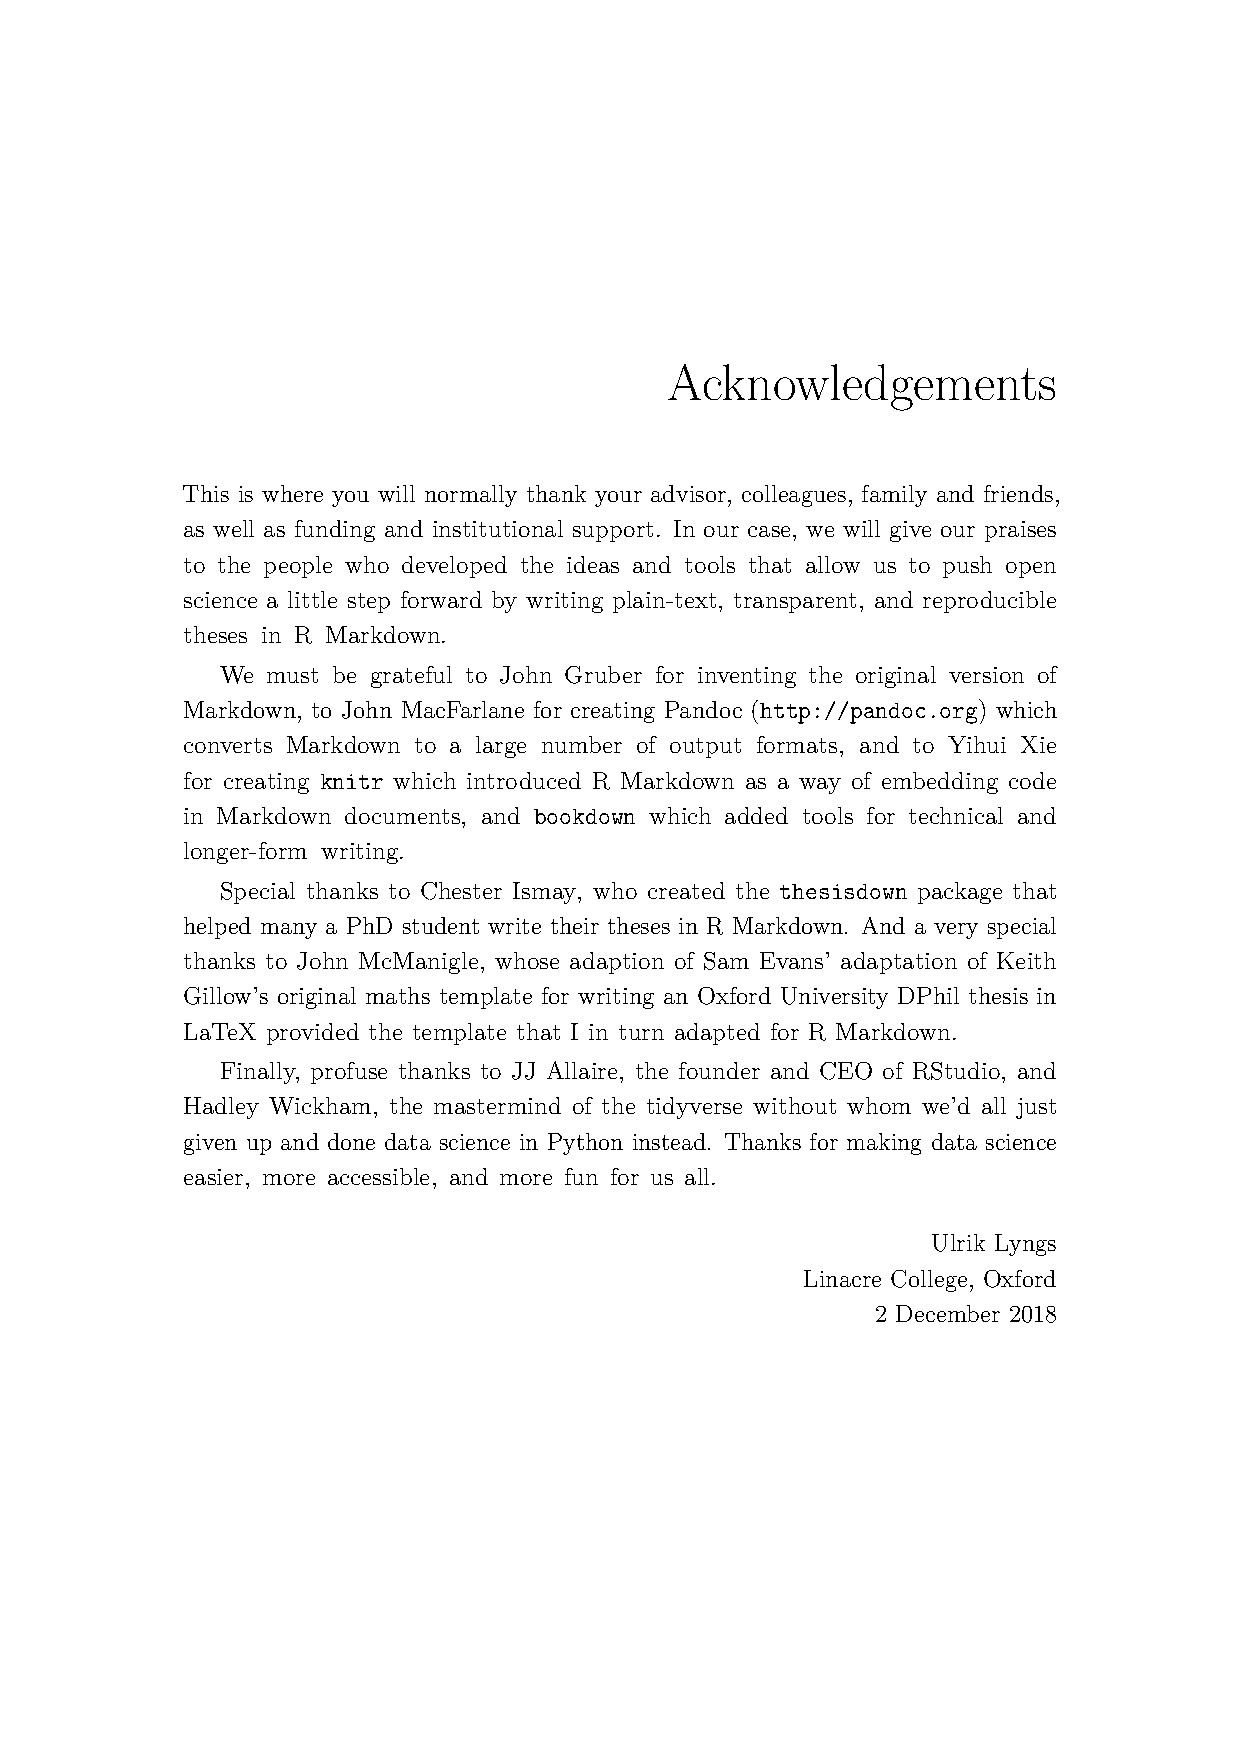
\includegraphics[width=0.32\linewidth]{figures/sample-content/alt_frontmatter_example/split/_000006.pdf}}

\hypertarget{troubleshooting}{%
\chapter{Troubleshooting}\label{troubleshooting}}

This chapter describes common errors you may run into, and how to fix them.

\hypertarget{error-failed-to-build-the-bibliography-via-biber}{%
\section{Error: Failed to build the bibliography via biber}\label{error-failed-to-build-the-bibliography-via-biber}}

This can happen if you've had a failed build, perhaps in relation to RStudio shutting down abruptly.

Try doing this:

\begin{enumerate}
\def\labelenumi{\arabic{enumi}.}
\tightlist
\item
  type \texttt{make\ clean-knits} in the terminal tab (or run \texttt{file.remove(list.files(pattern\ =\ "*.(log\textbar{}mtc\textbar{}maf\textbar{}aux\textbar{}bbl\textbar{}blg\textbar{}xml)"))} in the R console) to clean up files generated by LaTeX during a build
\item
  restart your computer
\end{enumerate}

If this does not solve the problem, try using the \href{https://www.overleaf.com/learn/latex/Bibliography_management_with_natbib}{natbib} LaTeX package instead of \href{https://www.overleaf.com/learn/latex/Articles/Getting_started_with_BibLaTeX}{biblatex} for handling references.
To do this, go to \textbf{index.Rmd} and

\begin{enumerate}
\def\labelenumi{\arabic{enumi}.}
\tightlist
\item
  set \texttt{use-biblatex:\ false} and \texttt{use-natbib:\ true}
\item
  set \texttt{citation\_package:\ natbib} under
\end{enumerate}

\begin{Shaded}
\begin{Highlighting}[]
\FunctionTok{output}\KeywordTok{:}
\AttributeTok{  bookdown:}\FunctionTok{:pdf_book}\KeywordTok{:}
\AttributeTok{    }\FunctionTok{citation_package}\KeywordTok{:}\AttributeTok{ natbib}
\end{Highlighting}
\end{Shaded}

\begin{savequote}
Alles Gescheite ist schon gedacht worden.\\
Man muss nur versuchen, es noch einmal zu denken.

All intelligent thoughts have already been thought;\\
what is necessary is only to try to think them again.
\qauthor{--- Johann Wolfgang von Goethe \autocite{von_goethe_wilhelm_1829}}\end{savequote}



\hypertarget{conclusion}{%
\chapter*{Conclusion}\label{conclusion}}
\addcontentsline{toc}{chapter}{Conclusion}

If we don't want Conclusion to have a chapter number next to it, we can add the \texttt{\{-\}} attribute.

\hypertarget{more-info}{%
\section*{More info}\label{more-info}}
\addcontentsline{toc}{section}{More info}

And here's some other random info:
the first paragraph after a chapter title or section head \emph{shouldn't be} indented, because indents are to tell the reader that you're starting a new paragraph.
Since that's obvious after a chapter or section title, proper typesetting doesn't add an indent there.

This paragraph, by contrast, \emph{will} be indented as it should because it is not the first one after the `More info' heading.
All hail LaTeX. (If you're reading the HTML version, you won't see any indentation - have a look at the PDF version to understand what in the earth this section is babbling on about).

\startappendices

\hypertarget{chap:appendix_a}{%
\chapter{Backpropagation with Binary Cross-Entropy}\label{chap:appendix_a}}

Let's consider a simple binary classification task. It is common to use a network with a single logistic output with the binary cross-entropy loss function and for the sake of simplicity, let's assume that there is only one hidden layer.
\[
\begin{aligned}
BCE=-\sum_{i=1}^{n o u t}\left(y_i \log \left(\hat{y}_i \right)+\left(1-y_i\right) \log \left(1-\hat{y}_i\right)\right)
\end{aligned}
\]

Where \(y\) is the ground truth and \(\hat{y}\) is the output of the network. After having the loss function, let's continue with the forward pass.

\[
\begin{aligned} 
a_{k} &= h_{k-1} w_{k} + b_k \\
h_k &= f(a_{k})
\end{aligned}
\]

Where, \(w_k\) is the weight, \(b_{k}\) is the bias term, \(h_k\) is the output of the layer (which means that \(h_0 = X\) and \(h_2 = \hat{y}\)) and f is the non linear function. Please note that for last layer logistic function is used whereas for hidden layer reLU is used as non linear functions.\\
We can compute the derivative of the weights by using the chain rule.

\[
\begin{aligned} 
\frac{\partial BCE}{\partial w_{2}}=\frac{\partial BCE}{\partial \hat{y}} \frac{\partial \hat{y}}{\partial a_{2}} \frac{\partial a_{2}}{\partial w_{2}}
\end{aligned}
\]

Computing each factor in the term, we have:
\[
\begin{aligned}
\frac{\partial BCE}{\partial \hat{y}} &=\frac{-y}{\hat{y}}+\frac{1-y}{1-\hat{y}} \\
&=\frac{\hat{y}-y}{\hat{y}\left(1-\hat{y}\right)} \\
\frac{\partial \hat{y}}{\partial a_{2}} &=\hat{y}\left(1-\hat{y}\right) \\
\frac{\partial a_{2}}{\partial w_{2}} &=h_{1}^T
\end{aligned}
\]
Which gives us:
\[
\frac{\partial BCE}{\partial w_{2}}=h_{1}^T\left(\hat{y}-y\right)
\]
Derivative of the \(w_1\) concerning loss function can be calculated as the following:

\[
\begin{aligned} 
\frac{\partial BCE}{\partial w_{1}}=\frac{\partial BCE}{\partial h_1} \frac{\partial h_1}{\partial a_{1}} \frac{\partial a_{1}}{\partial w_{1}}
\end{aligned}
\]
Compute each factor in the term again, we have:

\[
\begin{aligned}
\frac{\partial BCE}{\partial h_1} &= \frac{\partial BCE}{\partial \hat{y}} \frac{\partial \hat{y}}{\partial a_{2}} \frac{\partial a_{2}}{\partial h_{1}}  \\
&= \left(\hat{y}-y\right) w_{2}^T \\
\frac{\partial h_1}{\partial a_{1}} &=f'(a_1) \\
\frac{\partial a_{1}}{\partial h_{1}} &=X^T
\end{aligned}
\]
Which gives us:
\[
\begin{aligned}
\frac{\partial BCE}{\partial w_{1}}= \left(X\right)^T\left(\hat{y}-y\right)\left(w_{2}^T\right) \odot f'(a_1)
\end{aligned}
\]
Where \(\odot\) is element-wise multiplication, similarly, bias terms can be calculated by following:

\[
\begin{aligned} 
\frac{\partial BCE}{\partial b_{2}}&=\frac{\partial BCE}{\partial \hat{y}} \frac{\partial \hat{y}}{\partial a_{2}} \frac{\partial a_{2}}{\partial b_{2}} \\
&= \left(\hat{y}-y\right)
\end{aligned}
\]

\[
\begin{aligned} 
\frac{\partial BCE}{\partial b_{1}}&=\frac{\partial BCE}{\partial h_1} \frac{\partial h_1}{\partial a_{1}} \frac{\partial a_{1}}{\partial b_{1}} \\
&= \left(\hat{y}-y\right)\left(w_{2}^T\right) \odot f'(a_1)
\end{aligned}
\]
After having all these results, we can update the parameters (weights and biases) using gradient descent and its variants.

\hypertarget{reproducibility}{%
\chapter{Reproducibility}\label{reproducibility}}


%%%%% REFERENCES
\setlength{\baselineskip}{0pt} % JEM: Single-space References

{\renewcommand*\MakeUppercase[1]{#1}%
\printbibliography[heading=bibintoc,title={\bibtitle}]}


\end{document}
